
%%%%%%%%%%%%%%%%%%%%%%%%%%%%%%%%%%%%%%%%%
% Beamer Presentation
% LaTeX Template
% Version 1.0 (10/11/12)
%
% This template has been downloaded from:
% http://www.LaTeXTemplates.com
%
% License:
% CC BY-NC-SA 3.0 (http://creativecommons.org/licenses/by-nc-sa/3.0/)
%%%%%%%%%%%%%%%%%%%%%%%%%%%%%%%%%%%%%%%%%

%----------------------------------------------------------------------------------------
%	PACKAGES AND THEMES
%------------------------------------------------s----------------------------------------

\documentclass{beamer}

% salem colors
\definecolor{burntorange}{rgb}{0.968, 0.549, 0.114}
\definecolor{burntorangedark}{rgb}{0.486, 0.306, 0.102}
\definecolor{lightblue}{rgb}{0.161, 0.471, 1}
\definecolor{lightbluedark}{rgb}{0.125, 0.271, 0.510}

\definecolor{charcoal}{rgb}{0.21, 0.27, 0.31}
\definecolor{darkgray}{rgb}{0.3, 0.3, 0.3}
\definecolor{darkgrey}{rgb}{0.33, 0.33, 0.33}
\definecolor{cadmiumgreen}{rgb}{0.0, 0.42, 0.24}
\definecolor{brandeisblue}{rgb}{0.0, 0.44, 1.0}
\setbeamercolor{structure}{fg=darkgray}
\setbeamercolor{footline}{fg=darkgray}

\mode<presentation> {

\usepackage{amssymb, bm}
\usepackage{amsmath, amsfonts, amscd, epsfig, amssymb, amsthm, adjustbox}
\usepackage{textcomp}
\usepackage{graphicx}
\usepackage{setspace}
\usepackage{enumitem}
\setlist[itemize]{itemsep=9pt, label={--}}

\usepackage{anyfontsize}
\usepackage[utf8]{inputenc}
\usepackage[T1]{fontenc}
\usepackage{tcolorbox}[most]
\usepackage{tikz}
\usepackage[T1]{fontenc}
\usepackage{booktabs}
\usepackage{colortbl}
\usepackage{multirow}
\usepackage{array}
\usepackage{longtable}
\usepackage{listings}
\usepackage{color}
\usepackage{bbold}
\pagecolor{white}
\usepackage{mathtools}
\newcolumntype{K}[1]{>{\centering\arraybackslash}p{#1}}
\newcolumntype{Q}[1]{>{\columncolor[gray]{0.8}\centering\arraybackslash}p{#1}}
\newcommand\eho{\stackrel{\mathclap{\small\mbox{$H_0$}}}{=}}


\newcommand\norm[1]{\left\lVert#1\right\rVert}
\newcommand\smalldp{\fontsize{9.4}{7.2}\selectfont}
\newcommand\smalldpp{\fontsize{8.5}{7.2}\selectfont}
\newcommand\smalldppgh{\fontsize{9.5}{7.2}\selectfont}
\newcolumntype{H}{>{\setbox0=\hbox\bgroup}c<{\egroup}@{}}
\newcommand{\X}{\mathbf{X}}

\usepackage{color}
\pagecolor{white}
\usepackage[final]{pdfpages}

\newcommand{\bo}[1]{\textcolor{burntorange}{#1}}
\newcommand{\bod}[1]{\textcolor{burntorangedark}{#1}}
\newcommand{\lb}[1]{\textcolor{lightblue}{#1}}
\newcommand{\lbd}[1]{\textcolor{lightbluedark}{#1}}
\newcommand{\dg}[1]{\textcolor{darkgray}{#1}}

\newcommand{\dbl}{\setstretch{1.25}}
\newcommand{\hlf}{\setstretch{1}}

\newcommand{\bl}{\color{lightblue}}
\newcommand{\rd}{\color{burntorange}}
\newcommand{\bk}{\color{black}}
\newcommand{\gr}{\color{green}}

\newcommand{\bb}{$\lb{{\small \bullet } }$ \hspace{0.5mm}}
\newcommand{\ba}{$\lb{{\small \rightarrow } }$ \hspace{0.5mm}}

\newcommand{\bs}[1]{\boldsymbol{#1}}
\newcommand{\mc}[1]{\mathcal{#1}}
\newcommand{\mr}[1]{\mathrm{#1}}
%\newcommand{\bm}[1]{\mathbf{#1}}
\newcommand{\ds}[1]{\mathds{#1}}

\newcommand{\bi}{\begin{itemize}}
\newcommand{\ib}{\end{itemize}}
\newcommand{\p}{\item}
\newcommand{\sk}{\vspace{.5cm}}

\newcommand{\sko}{\vspace{.1in}}
\newcommand{\skoo}{\vspace{.2in}}
\newcommand{\skooo}{\vspace{.3in}}
\newcommand{\hko}{\hspace{.1in}}
\newcommand{\hkoo}{\hspace{.2in}}
\newcommand{\hkooo}{\hspace{.3in}}

\newcommand{\gvn}{\; | \;}

\newcommand{\E}{\ds{E}}
\newcommand{\var}{\mr{var}}


% The Beamer class comes with a number of default slide themes
% which change the colors and layouts of slides. Below this is a list
% of all the themes, uncomment each in turn to see what they look like.
\usepackage{color}
\pagecolor{white}
\usepackage[final]{pdfpages}
\usetheme{default}

\setbeamertemplate{navigation symbols}{}
\setbeamertemplate{footline}[frame number]{}
\setbeamertemplate{footline}{}
 % To remove the navigation symbols from the bottom of all slides uncomment this line
}

\usepackage{graphicx} % Allows including images
\usepackage{booktabs} % Allows the use of \toprule, \midrule and \bottomrule in tables

%----------------------------------------------------------------------------------------
%	TITLE PAGE
%----------------------------------------------------------------------------------------

\setbeamertemplate{footline}{\scriptsize{\hfill\insertframenumber\vspace{-.2cm}\hspace*{.35cm}}} 
%\addtobeamertemplate{footline}{\hspace{4mm}\includegraphics[scale=0.006]{uchicago_shield} \vspace{-0.6cm}}{\vspace{1cm}}
\addtobeamertemplate{footline}{\vspace{-0.4cm}}{\vspace{0.5cm}}
\addtobeamertemplate{headline}{\vspace{2.5mm}\hspace{120mm}
%
\includegraphics[scale=0.05]{salem-S}\vspace{-8mm}
}
%\setbeamertemplate{frametitle}{{\vspace{3mm}}}


%
\includegraphics[scale=.5]{UTlogo.png} 

\title[]{\Large{Bias-variance tradeoff} \vspace{5mm}}

%'\subtitle{}

\author{David Puelz \\ \dg{\small The University of Austin}}
\institute[] % Your institution as it will appear on the bottom of every slide, may be shorthand to save space
{

}
\date{} % Date, can be changed to a custom date

\begin{document}

{\setbeamertemplate{footline}{}
\setbeamertemplate{headline}{}
\begin{frame}[noframenumbering]
\vspace{12mm}
%\centerline{
\includegraphics[scale=0.075]{salem-banner}}
\vspace{5mm}
\titlepage % Print the title page as the first slide
\end{frame}
}

%% Overview slide
%\begin{frame}
%\frametitle{Overview} % Table of contents slide, comment this block out to remove it
%\tableofcontents % Throughout your presentation, if you choose to use \section{} and \subsection{} commands, these will automatically be printed on this slide as an overview of your presentation
%\end{frame}

%---------------------------------------------------------------------------------------
%	PRESENTATION SLIDES
%----------------------------------------------------------------------------------------

%------------------------------------------------


%------------------------------------------------


\begin{frame}[plain]
\frametitle{Fitting a function to data}


Let's go back to fitting function with data. \\  \sk\sk

There was an interesting question ... \bo{How wiggly \dg{(or not wiggly)} should my functions be to generate reasonable predictions?} \\ \sk\sk

The answer is \lb{\underline{crucial}} for how we discover and build functions in the real-world.

 

\end{frame}




\begin{frame}[plain]
\frametitle{Remember the framing of our ``function fitting'' problem}
Predict a \bo{target variable $Y$} with \bo{input variables $X$}.\skooo 


\pause
\skoo

We can frame the problem by supposing $Y$ and $X$ are related in the following way:
$$
Y_i = \bo{f(}X_i\bo{)} + \epsilon_i
$$

\skoo
{To achieve our goal, we need to: {\it Learn or estimate} $\bo{f(\cdot)}$ from data. }


\end{frame}



\begin{frame}[plain]
\frametitle{Boston housing data}
\vspace{5mm}
\begin{itemize}
\item[] Predict \bo{median home value} with \bo{percent low economic status}.
\item[] \textcolor{white}{fill}
\end{itemize}
\vspace{-16mm}
\begin{center}
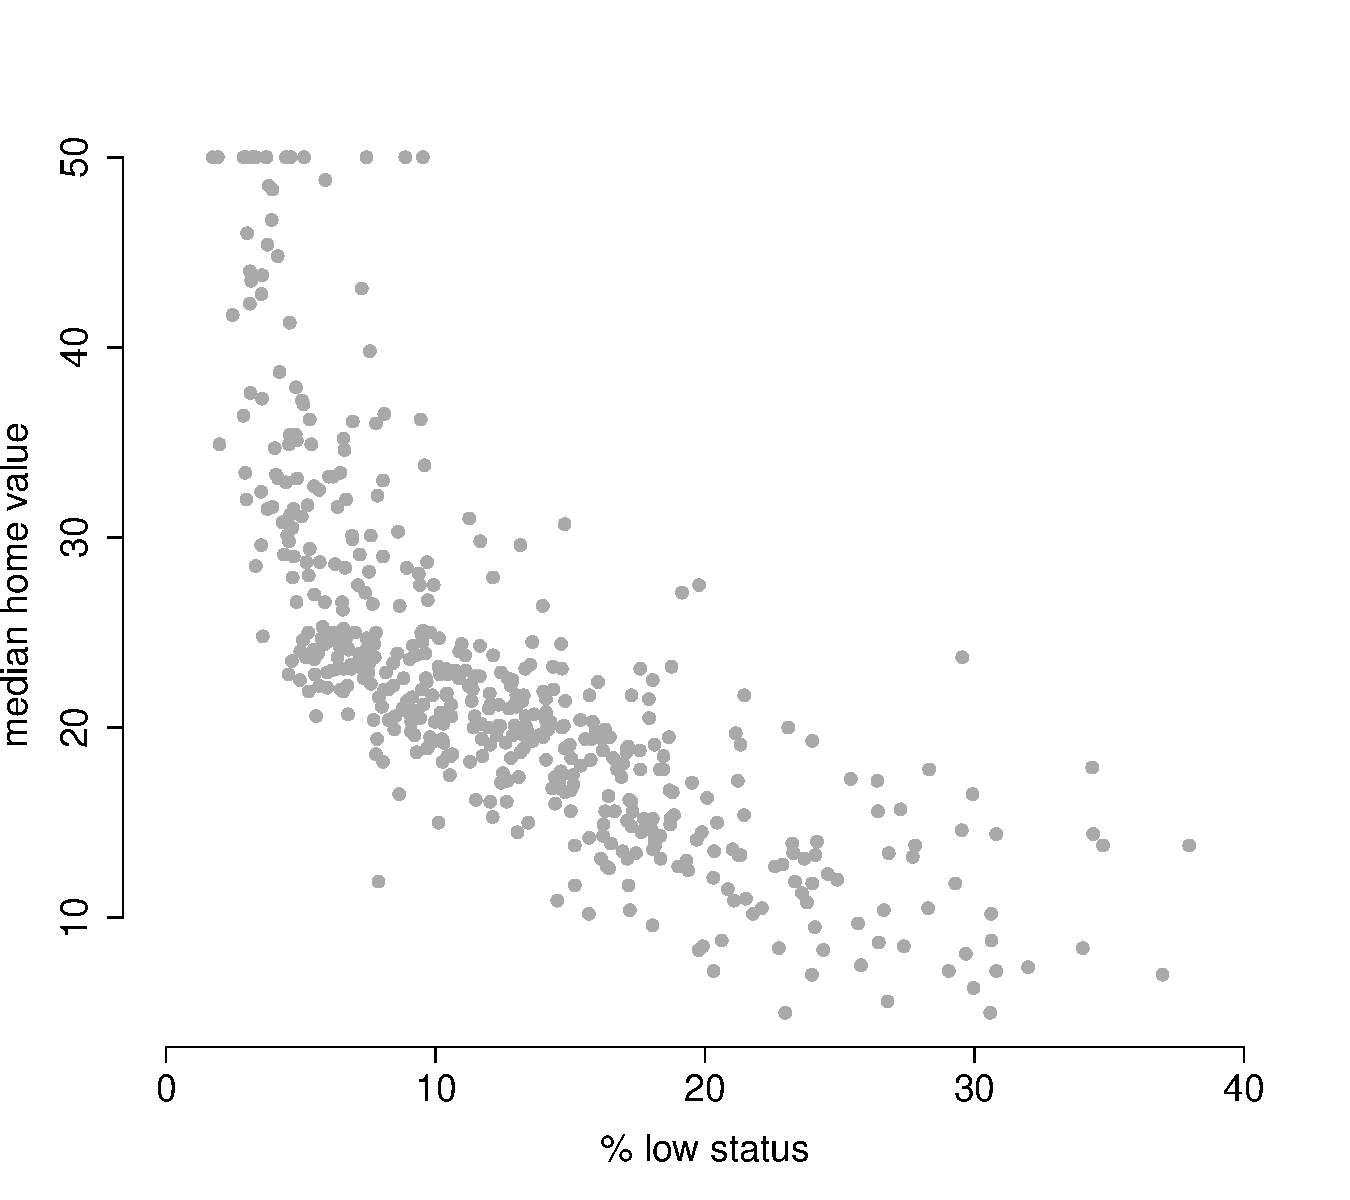
\includegraphics[scale=.39]{DaveBostonplot.pdf}
\end{center}

\end{frame}

\begin{frame}[plain]
\frametitle{Boston housing data}
\vspace{5mm}
\begin{itemize}
\item[] Prediction at \bo{\% low status} = 30? \textcolor{white}{fill}
\item[] \textcolor{white}{fill}
\end{itemize}
\vspace{-16mm}
\begin{center}
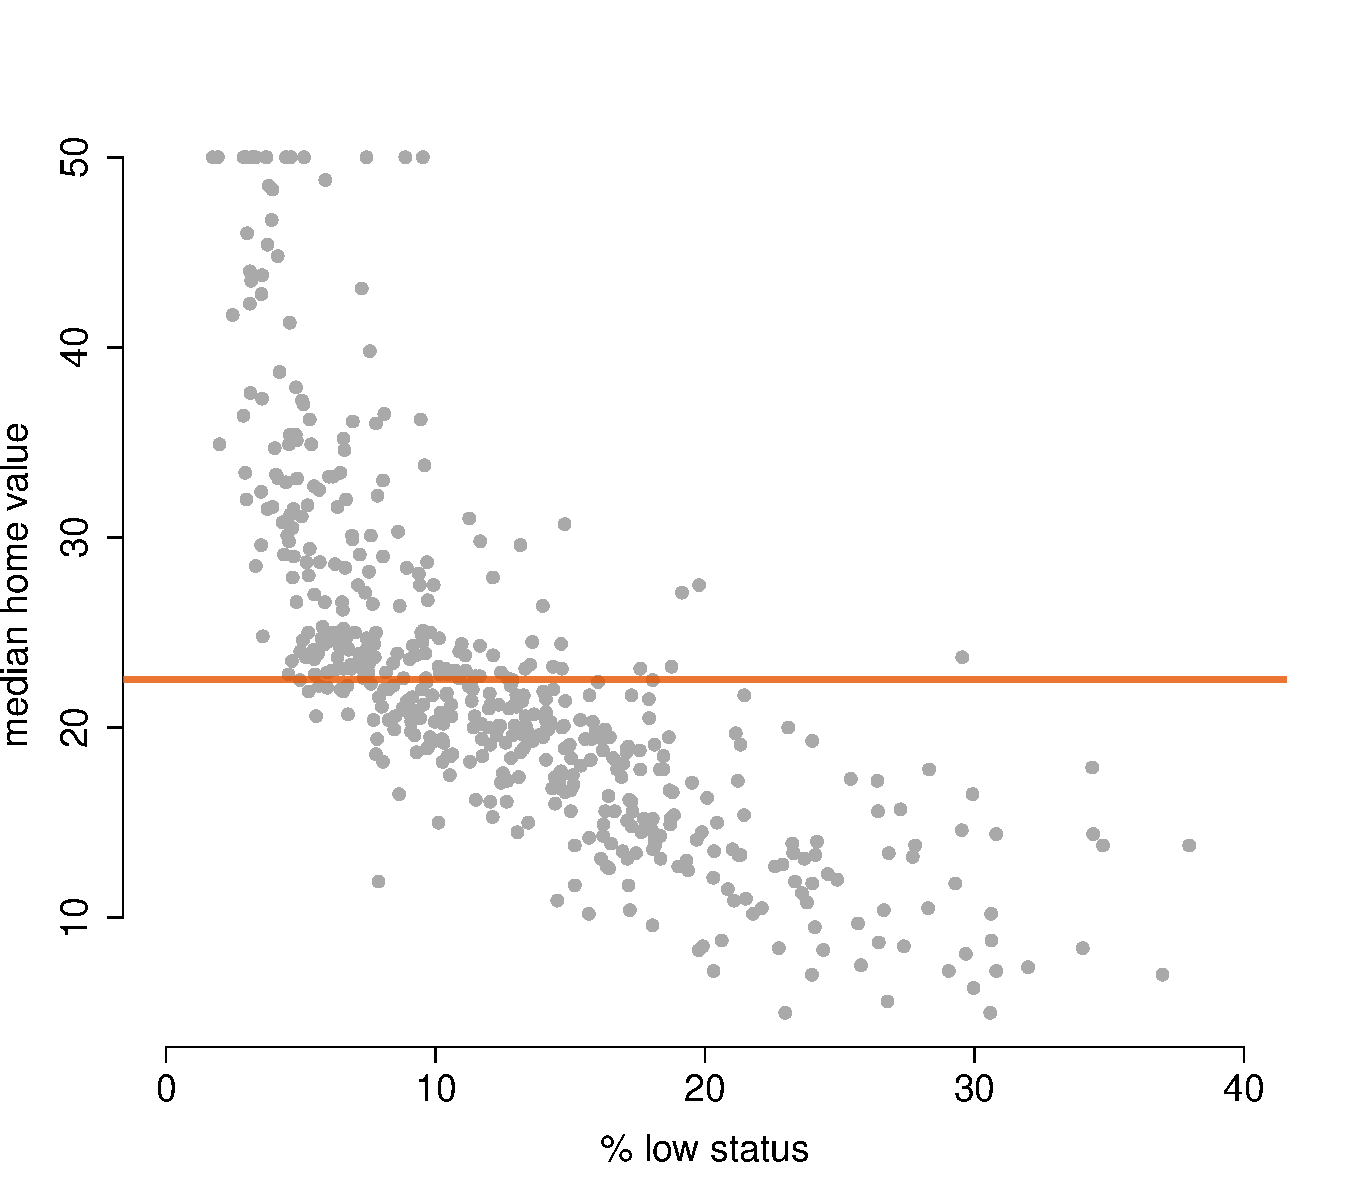
\includegraphics[scale=.39]{DaveBostonplot1.pdf}
\end{center}

\end{frame}

\begin{frame}[plain]
\frametitle{Boston housing data}
\vspace{5mm}
\begin{itemize}
\item[] Prediction at \bo{\% low status} = 30? \textcolor{white}{fill}
\item[] \textcolor{white}{fill}
\end{itemize}
\vspace{-16mm}
\begin{center}
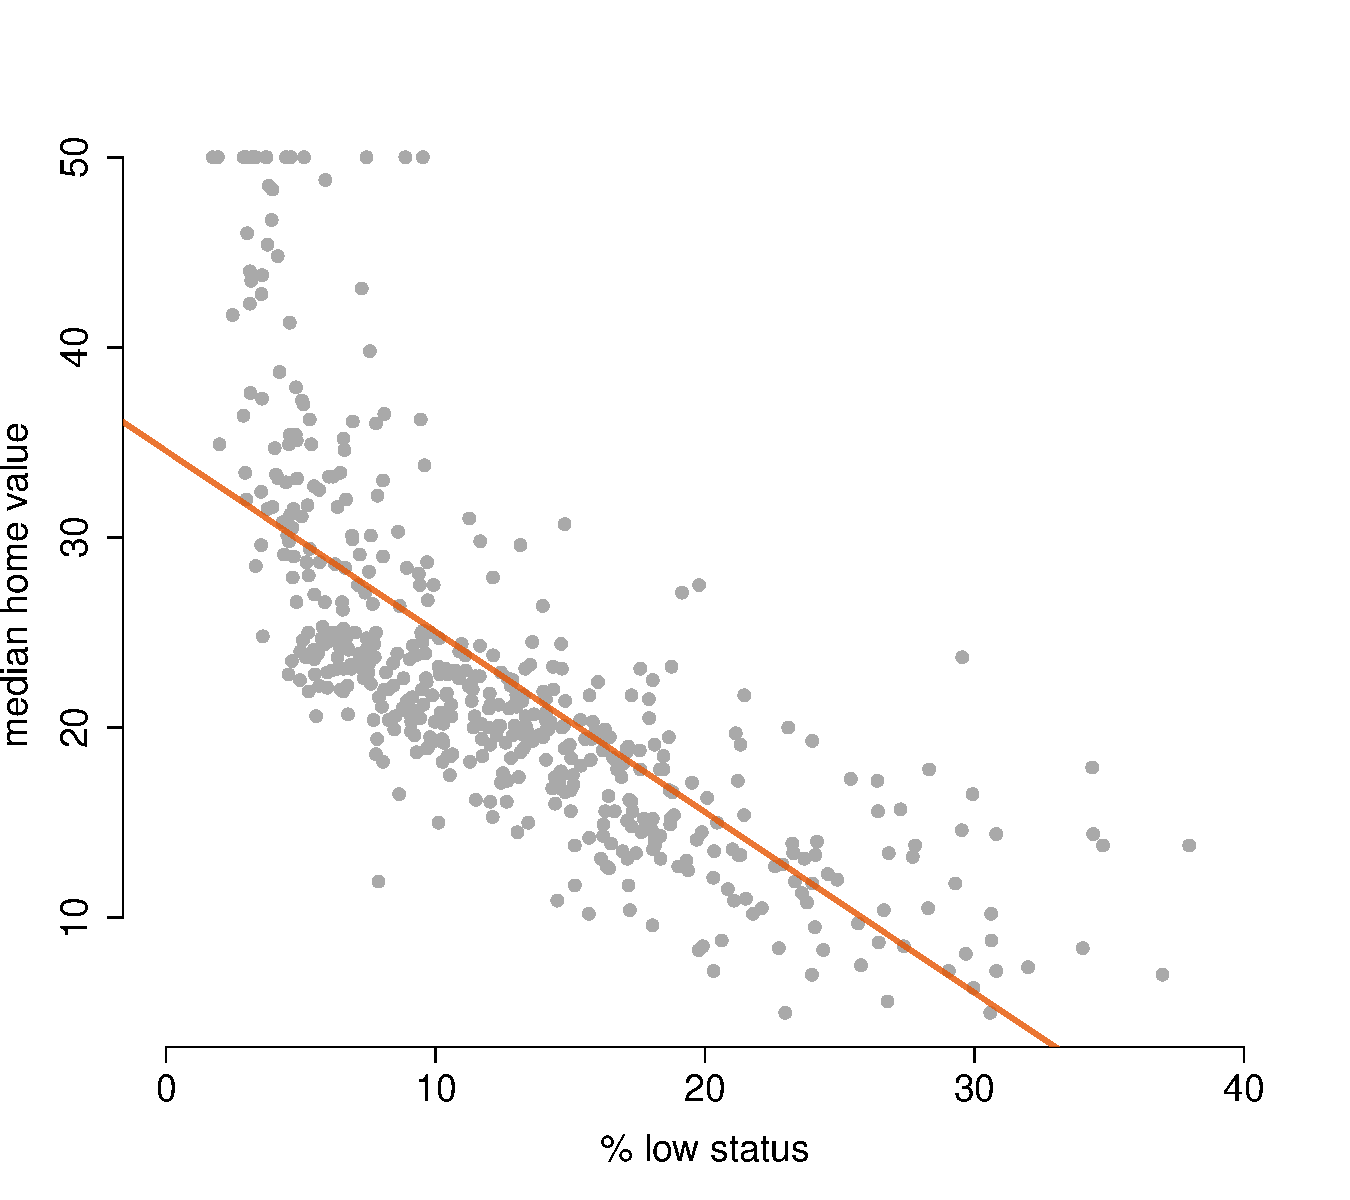
\includegraphics[scale=.39]{DaveBostonplot2.pdf}
\end{center}

\end{frame}


\begin{frame}[plain]
\frametitle{Boston housing data}
\vspace{5mm}
\begin{itemize}
\item[] Prediction at \bo{\% low status} = 30? \textcolor{white}{fill}
\item[] \textcolor{white}{fill}
\end{itemize}
\vspace{-16mm}
\begin{center}
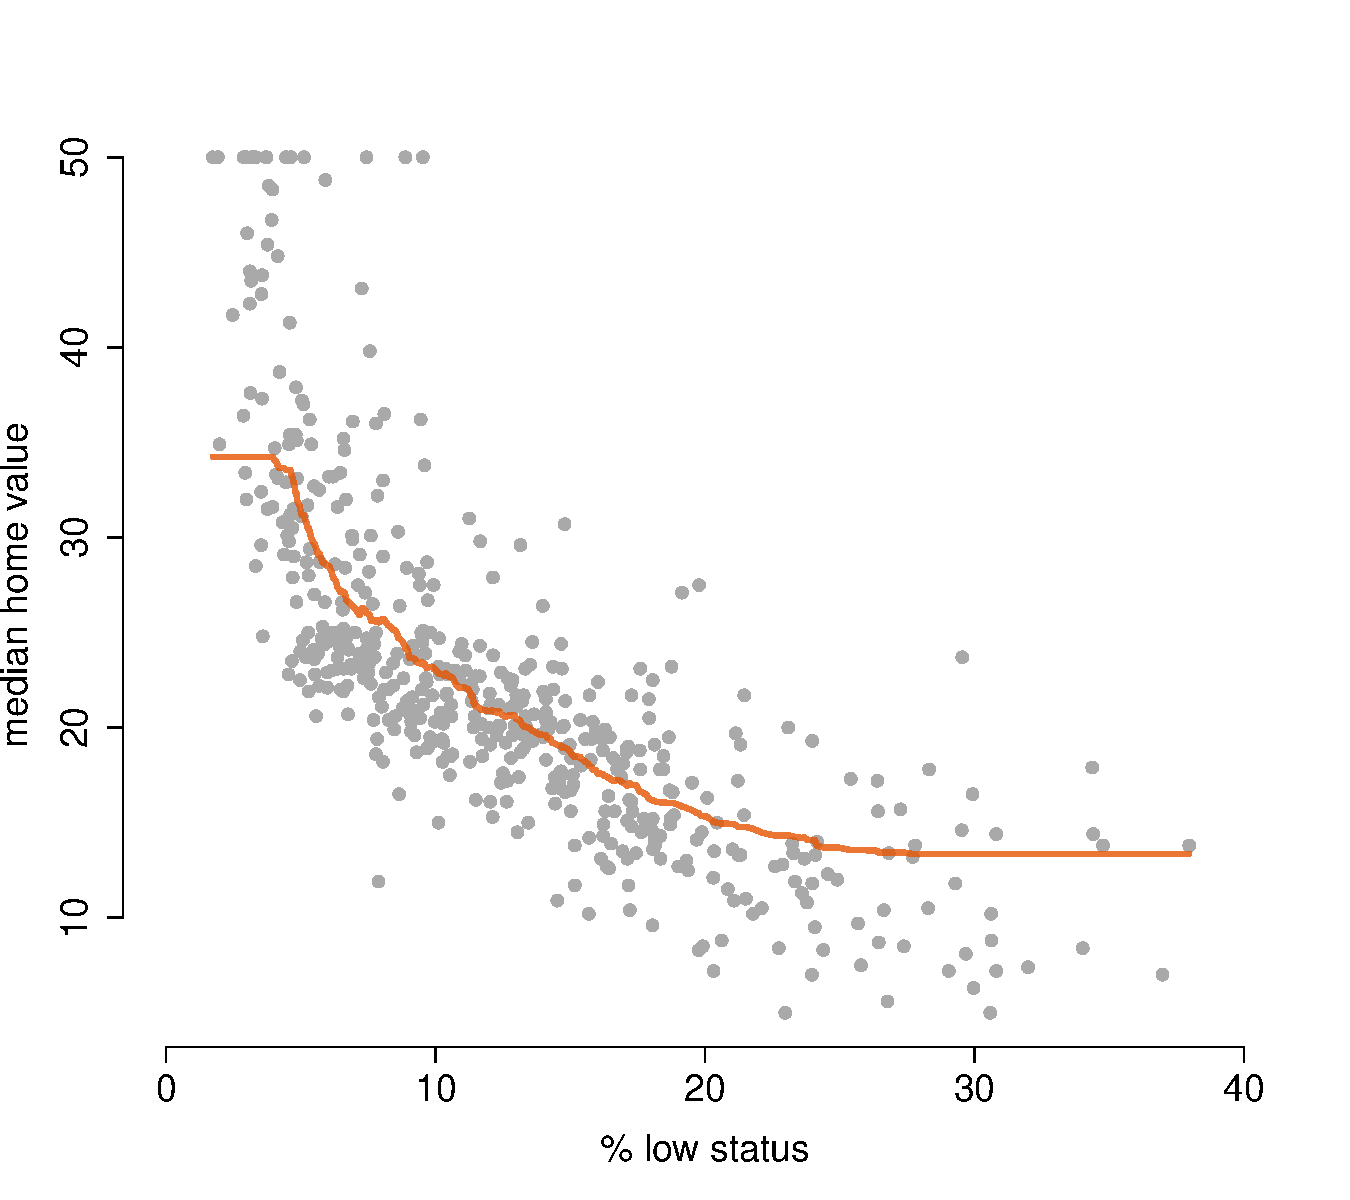
\includegraphics[scale=.39]{DaveBostonplot3.pdf}
\end{center}

\end{frame}

%\begin{frame}[plain]
%\frametitle{How do we estimate $\bo{f(\cdot)}$?}
%\vspace{7mm}
%1. Choose set of \underline{training data}: $(Y_{1},X_{1}), \dots,(Y_{N},X_{N})$.
%\\
%\pause
%\vspace{7mm}
%2. Fit $\bo{f(\cdot)}$ to training data using: \\
%%\vspace{7mm}
%%\begin{itemize}
%%\item Parametric model, or
%%\item Nonparametric model
%%\end{itemize} 
%\pause
%\vspace{7mm}
%3. Evaluate performance on \underline{testing data} and \textit{adjust}.
%
%\end{frame}



\begin{frame}[plain]
\frametitle{How do we estimate $\bo{f(\cdot)}$?}
\vspace{5mm}
\begin{itemize}
\item[] \bo{\lb{restrictive} fit, but \lb{simple} interpretation}.
\end{itemize}
\vspace{-9mm}
\begin{center}
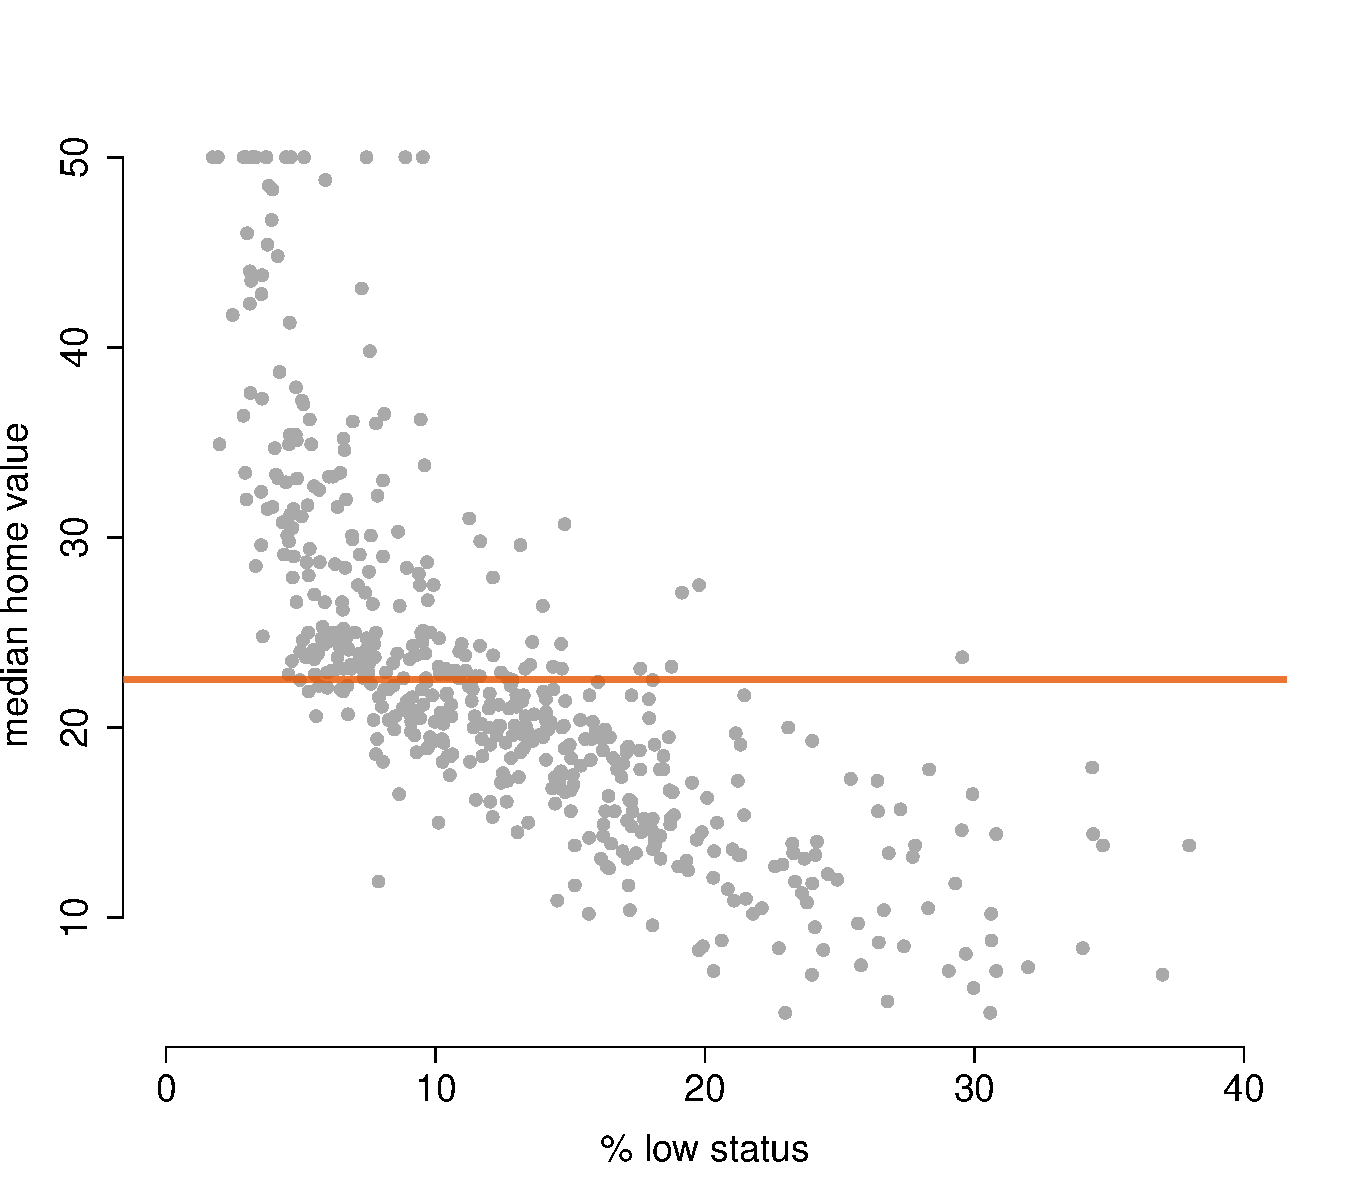
\includegraphics[scale=.39]{DaveBostonplot1.pdf}
\end{center}


\end{frame}

\begin{frame}[plain]
\frametitle{How do we estimate $\bo{f(\cdot)}$?}
\vspace{5mm}
\begin{itemize}
\item[] \bo{\lb{flexible} fit, but \lb{complex} interpretation}.
\end{itemize}
\vspace{-9mm}
\begin{center}
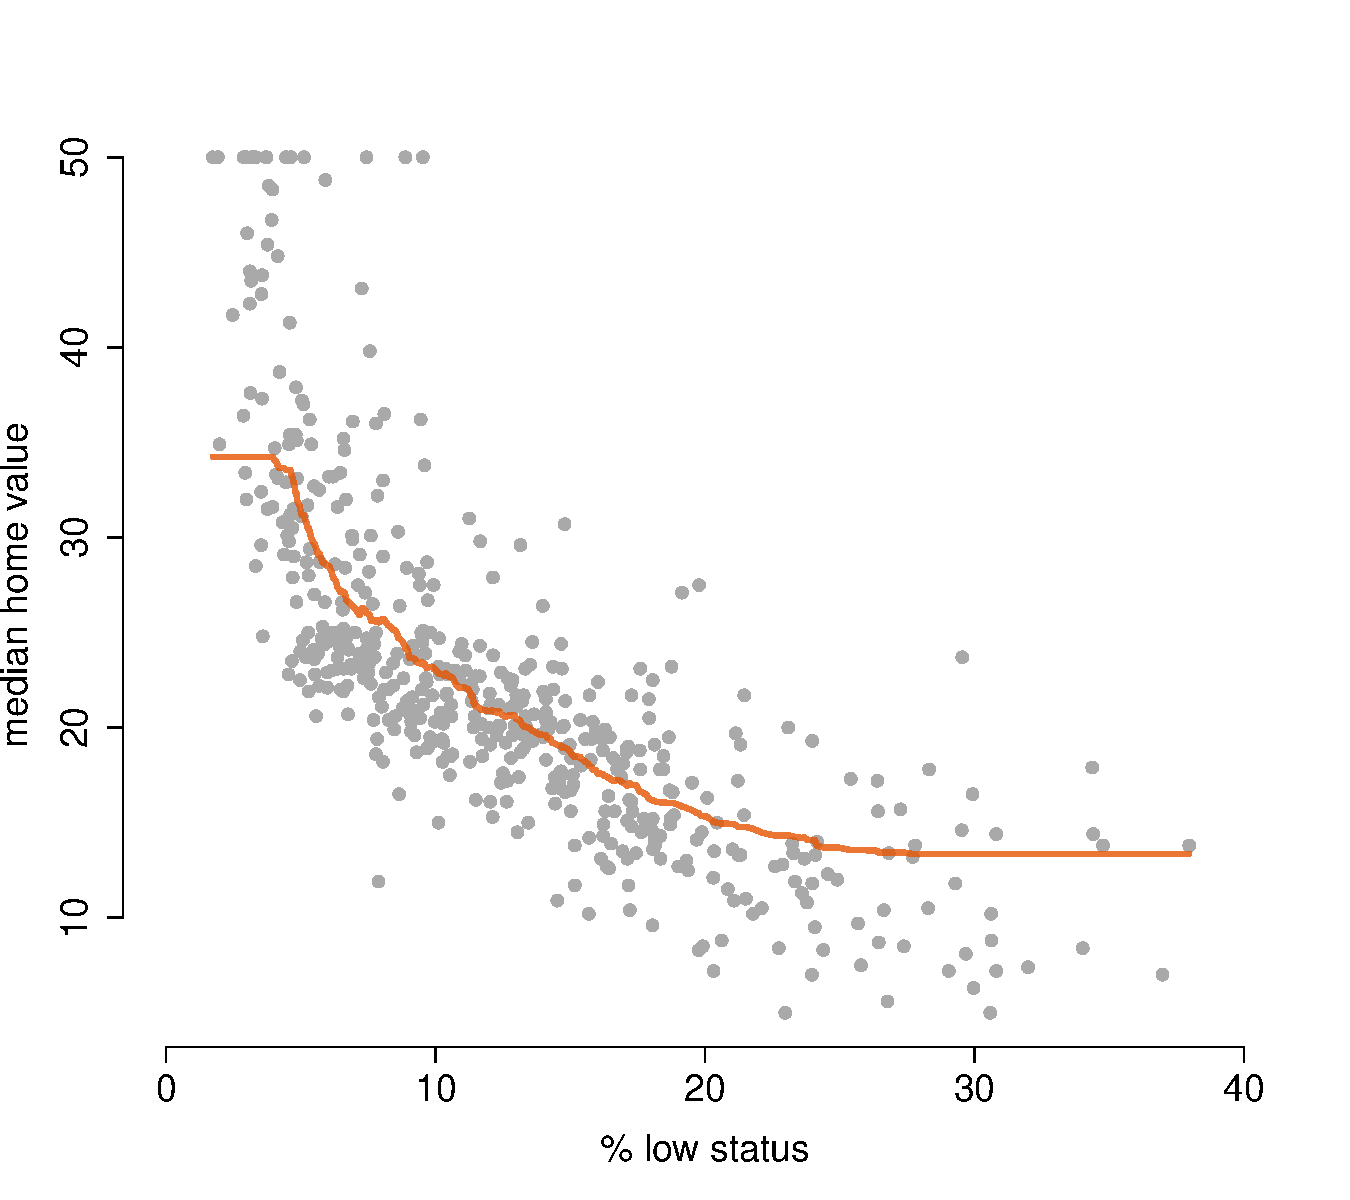
\includegraphics[scale=.39]{DaveBostonplot3.pdf}
\end{center}


\end{frame}


\begin{frame}[plain]
\frametitle{The challenge when estimating predictions $\bo{\widehat{f(\cdot)}}$}
\vspace{5mm}
\Large
Balancing \lb{{restrictiveness}} of function fit with simplicity of \lb{interpretation}.

\end{frame}

\begin{frame}[plain]
\frametitle{Let's look at k-nearest-neighbors (knn)}
\vspace{5mm}
	Prediction at point $x$, $\widehat{f(x)} =$ average of k nearest points around $x$. \\ \vspace{9mm}\pause
Let's look at $\bo{k=20}$ ...
\end{frame}

\begin{frame}[plain]
\frametitle{knn with $\bo{k=20}$}
\vspace{-8mm}
\begin{center}
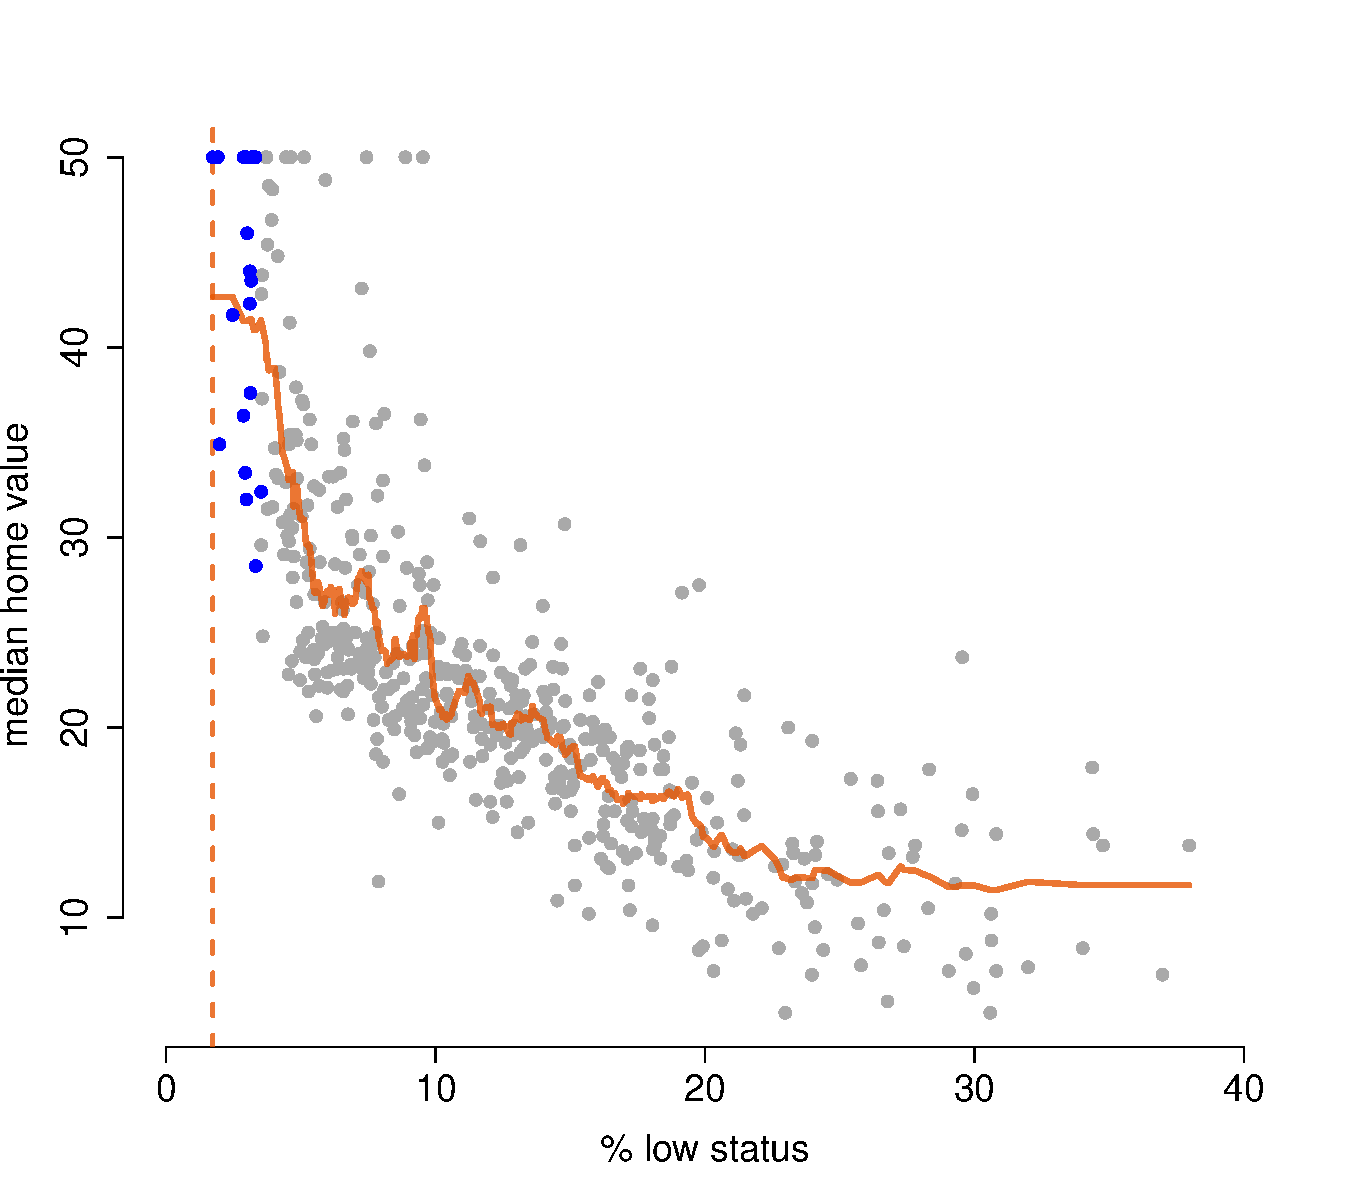
\includegraphics[scale=.44]{DaveBostonplotk=20ii=1.pdf}
\end{center}
\end{frame}

\begin{frame}[plain]
\frametitle{knn with $\bo{k=20}$}
\vspace{-8mm}
\begin{center}
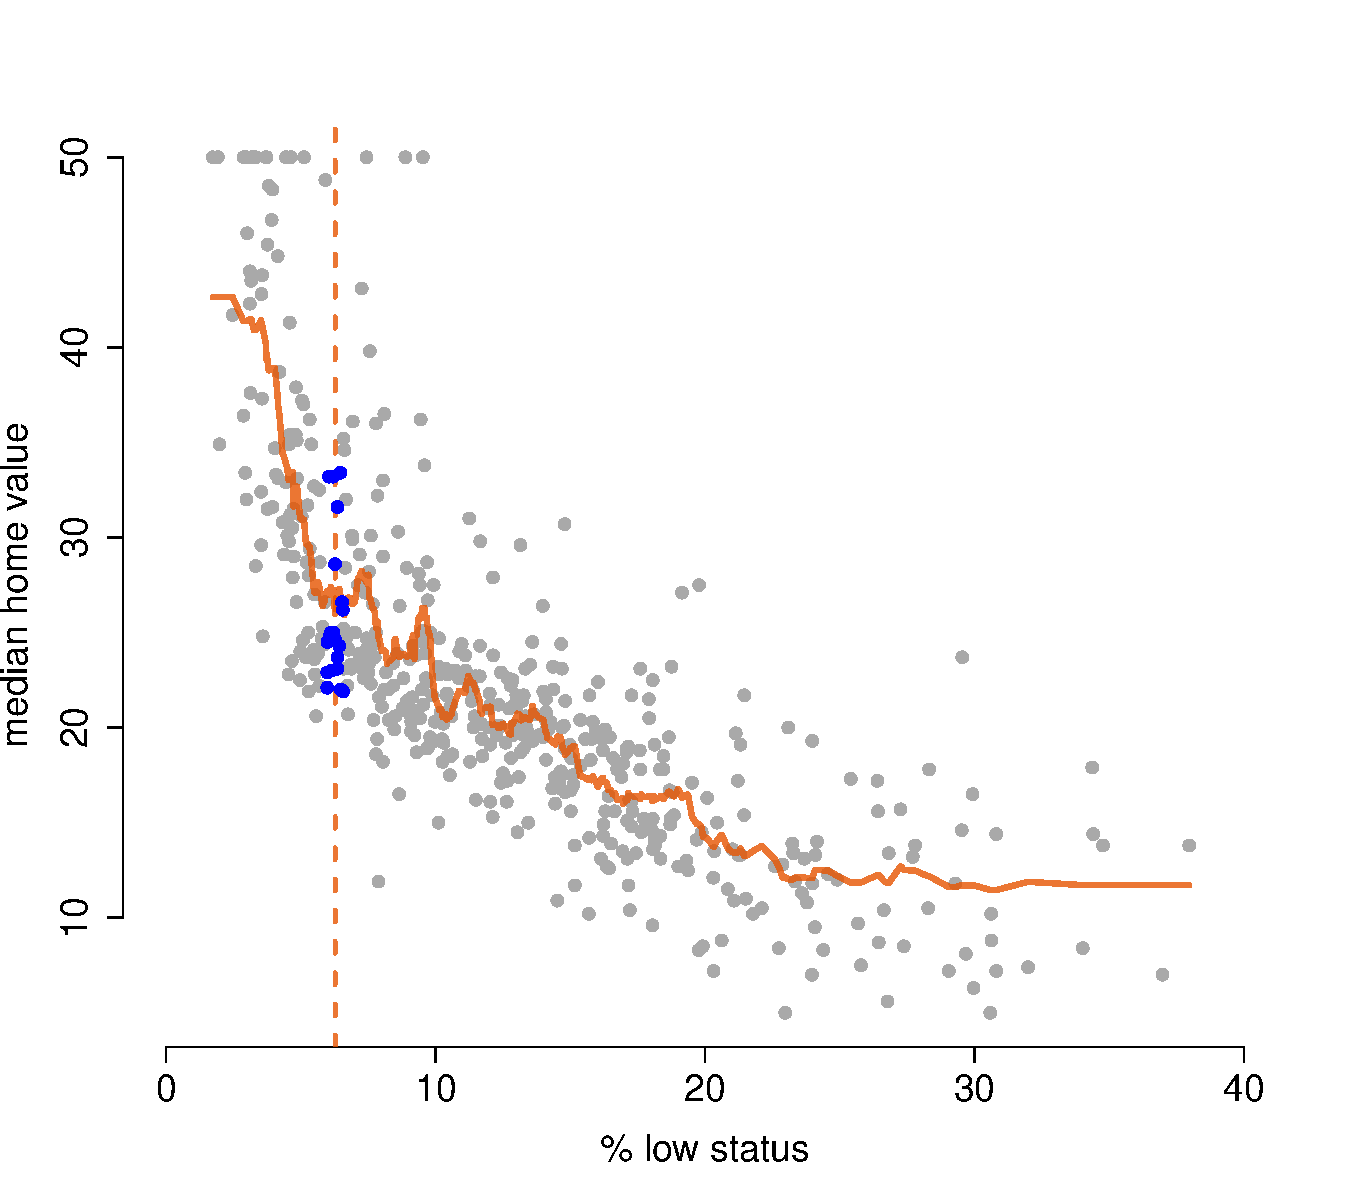
\includegraphics[scale=.44]{DaveBostonplotk=20ii=2.pdf}
\end{center}
\end{frame}

\begin{frame}[plain]
\frametitle{knn with $\bo{k=20}$}
\vspace{-8mm}
\begin{center}
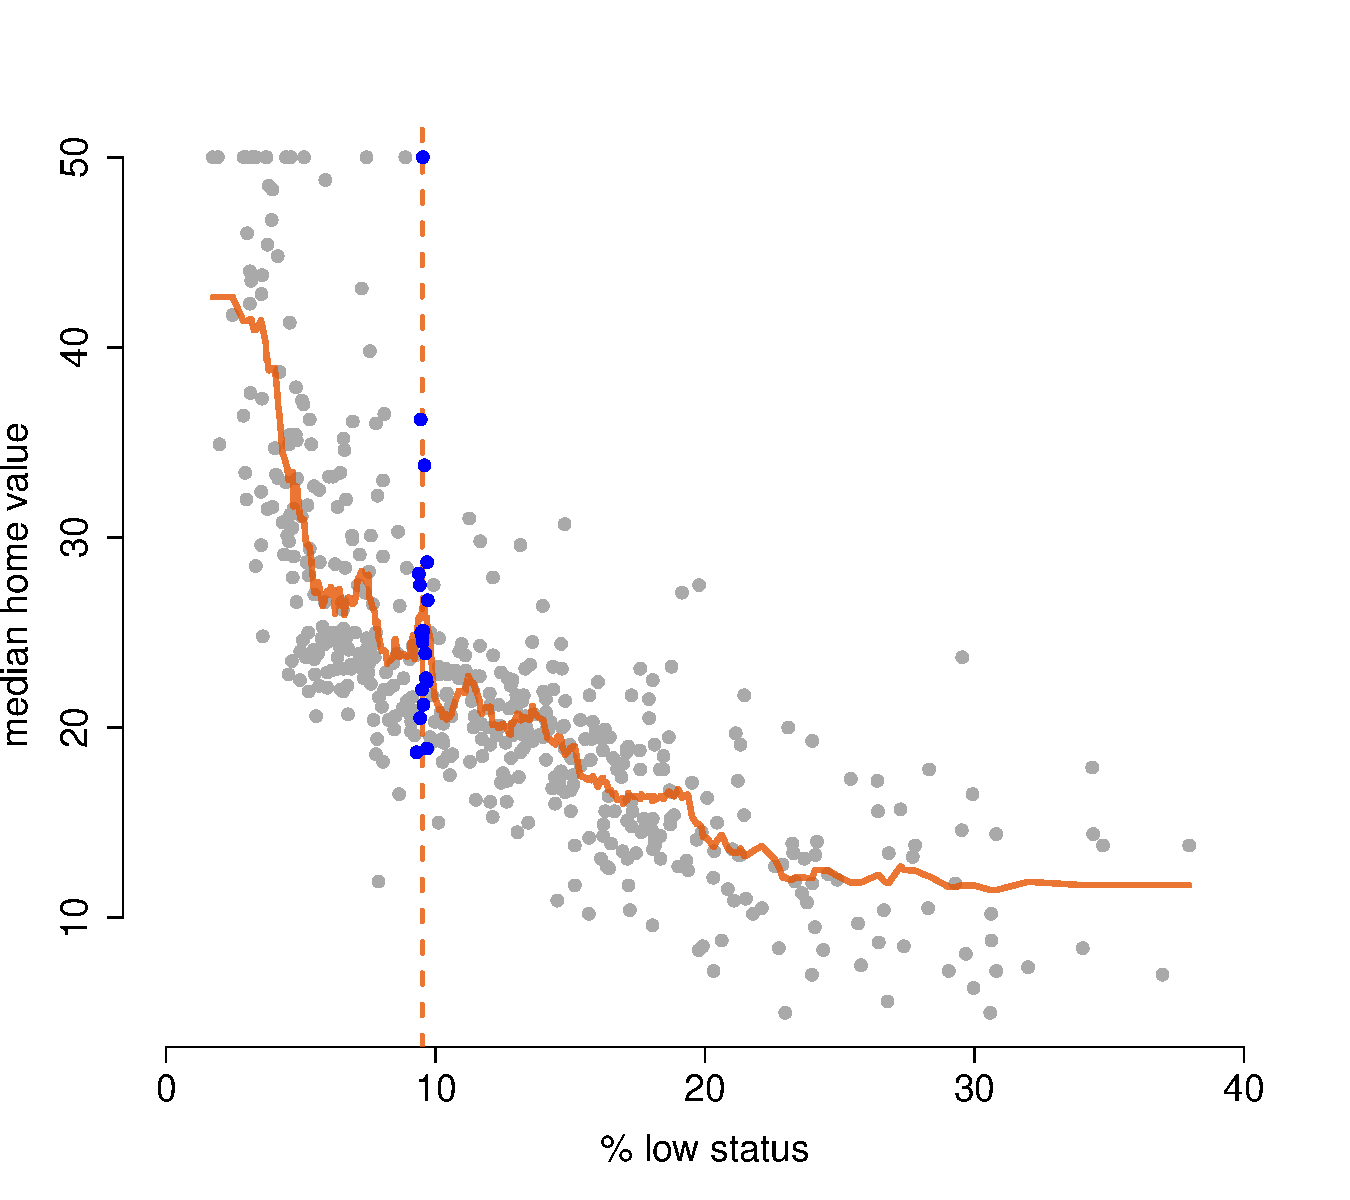
\includegraphics[scale=.44]{DaveBostonplotk=20ii=3.pdf}
\end{center}
\end{frame}

\begin{frame}[plain]
\frametitle{knn with $\bo{k=20}$}
\vspace{-8mm}
\begin{center}
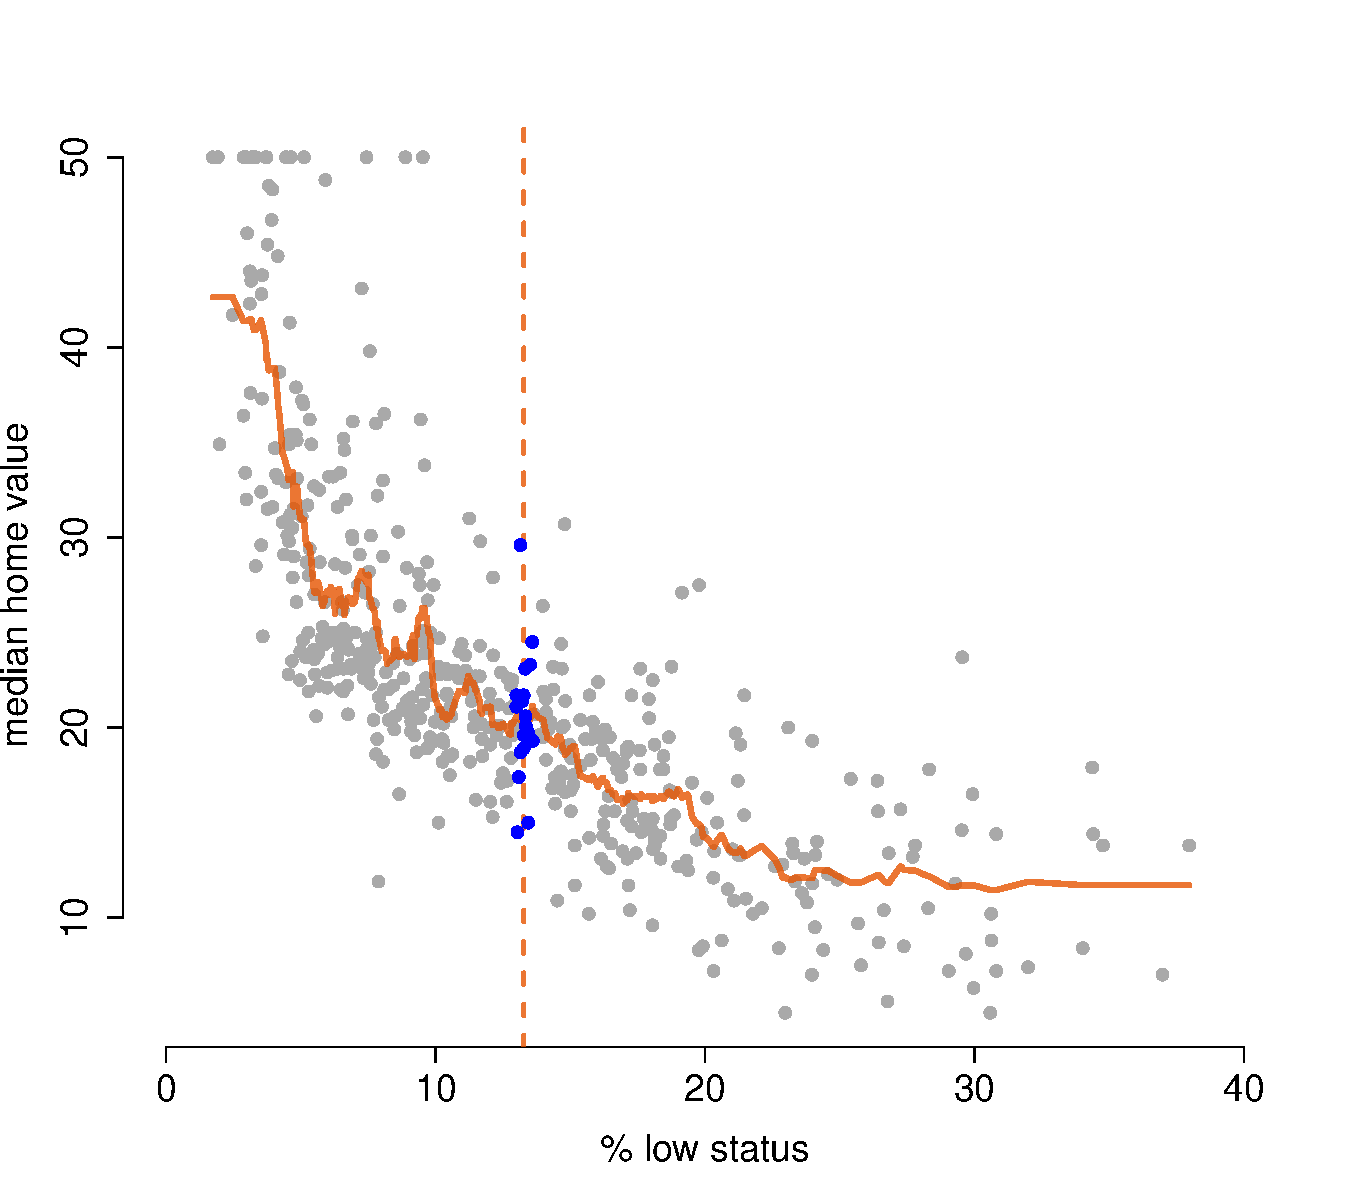
\includegraphics[scale=.44]{DaveBostonplotk=20ii=4.pdf}
\end{center}
\end{frame}

\begin{frame}[plain]
\frametitle{knn with $\bo{k=20}$}
\vspace{-8mm}
\begin{center}
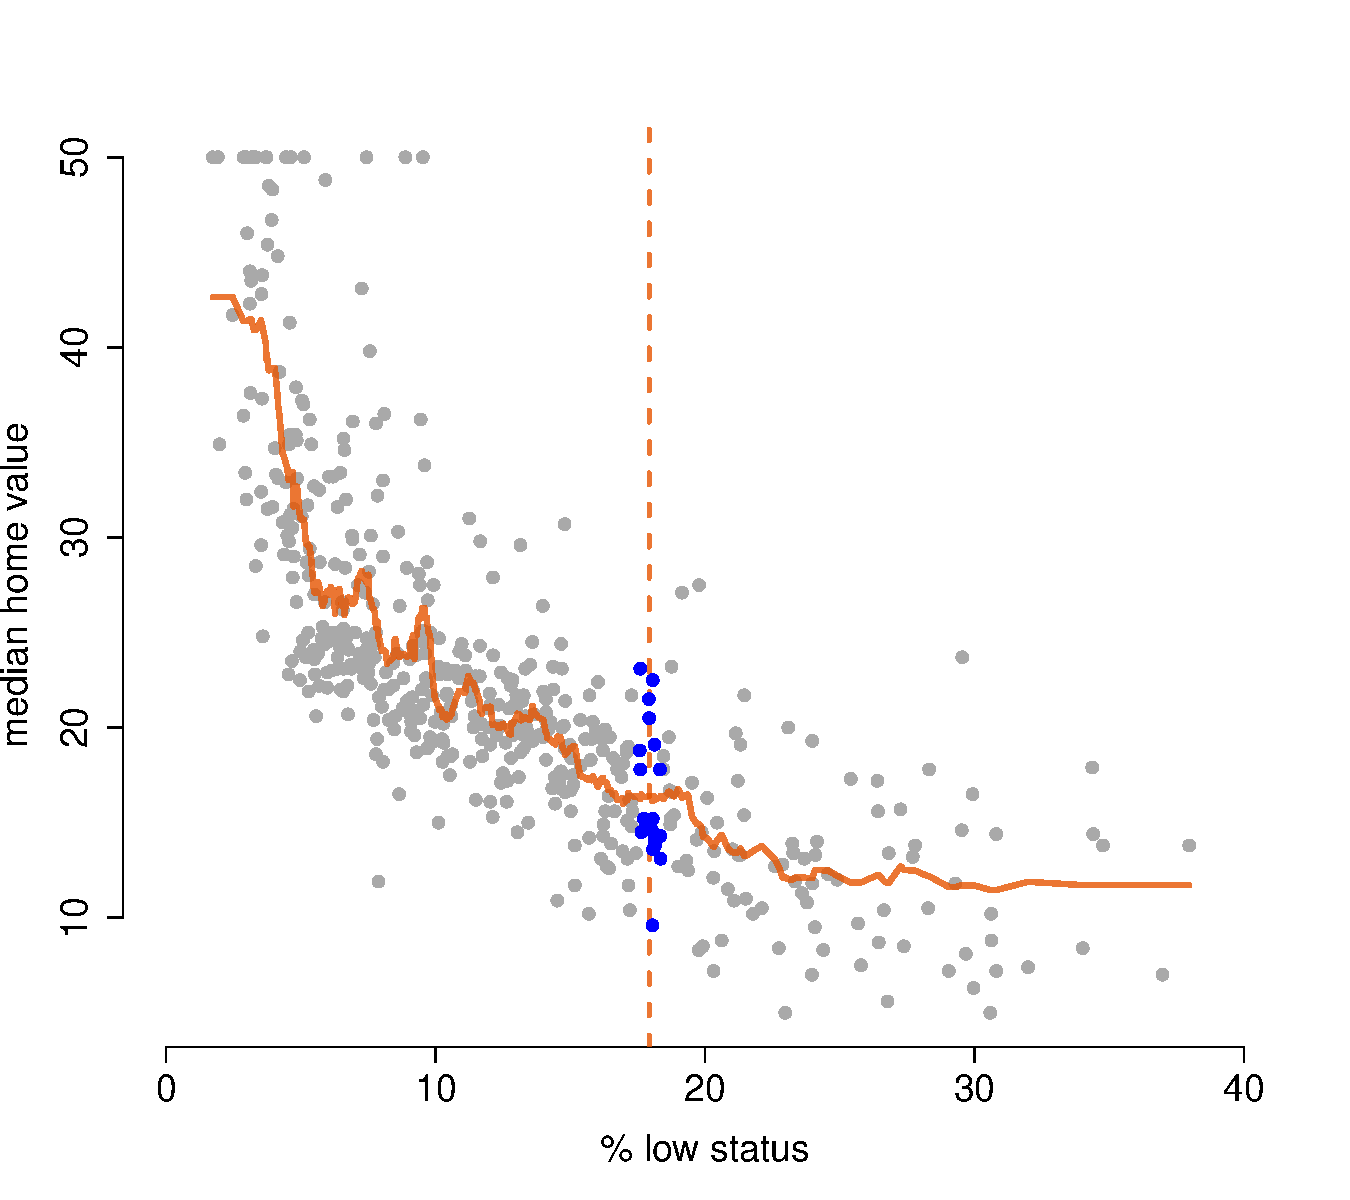
\includegraphics[scale=.44]{DaveBostonplotk=20ii=5.pdf}
\end{center}
\end{frame}

\begin{frame}[plain]
\frametitle{knn with $\bo{k=20}$}
\vspace{-8mm}
\begin{center}
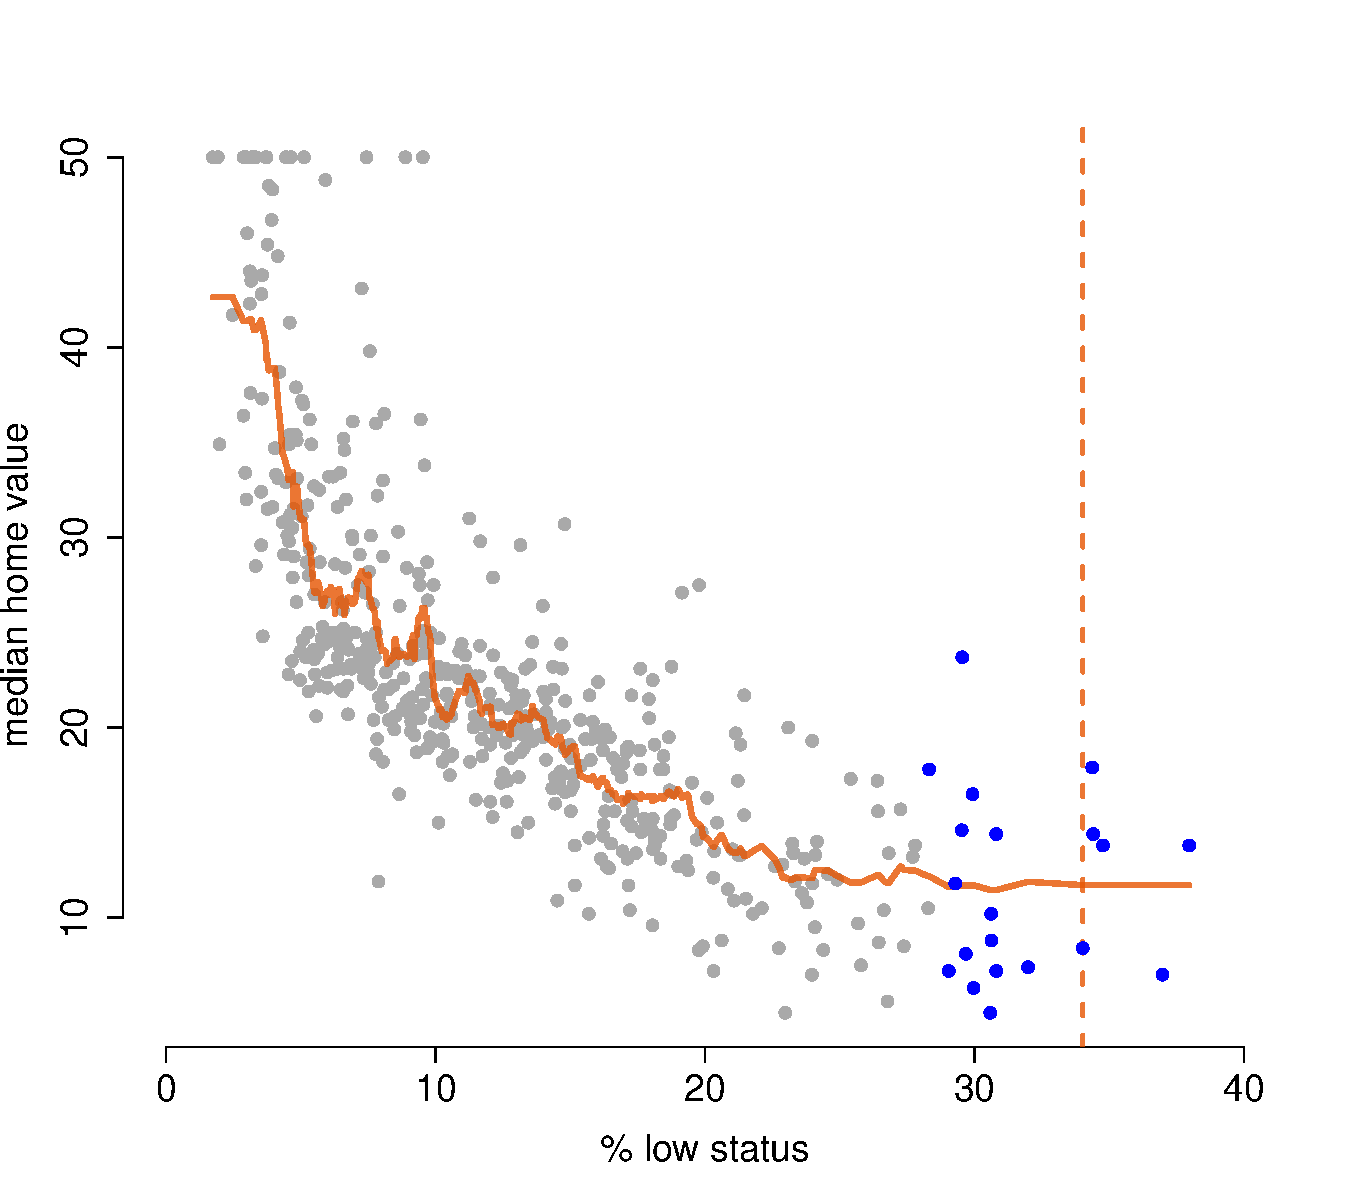
\includegraphics[scale=.44]{DaveBostonplotk=20ii=6.pdf}
\end{center}
\end{frame}

\begin{frame}[plain]
\frametitle{Why don't I choose $\bo{k=2}$ instead?}
\vspace{-8mm}
\begin{center}
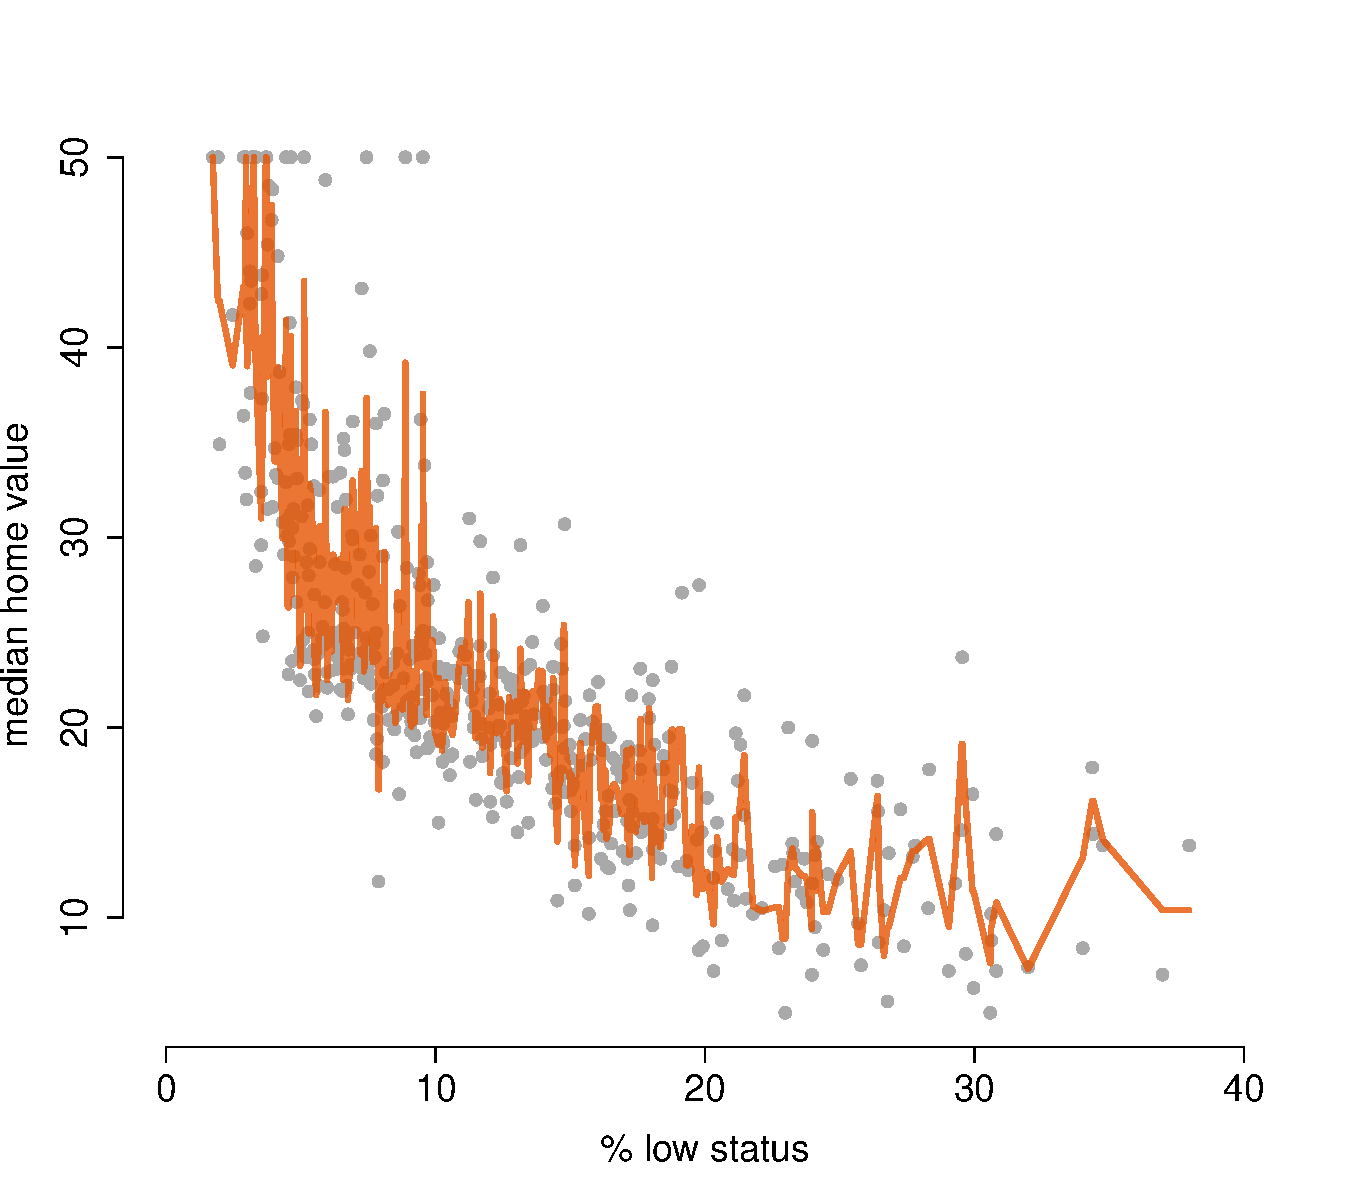
\includegraphics[scale=.44]{DaveBostonplotk=2i=1.pdf}
\end{center}
\end{frame}

\begin{frame}[plain]
\frametitle{or $\bo{k=10}$ ...}
\vspace{-8mm}
\begin{center}
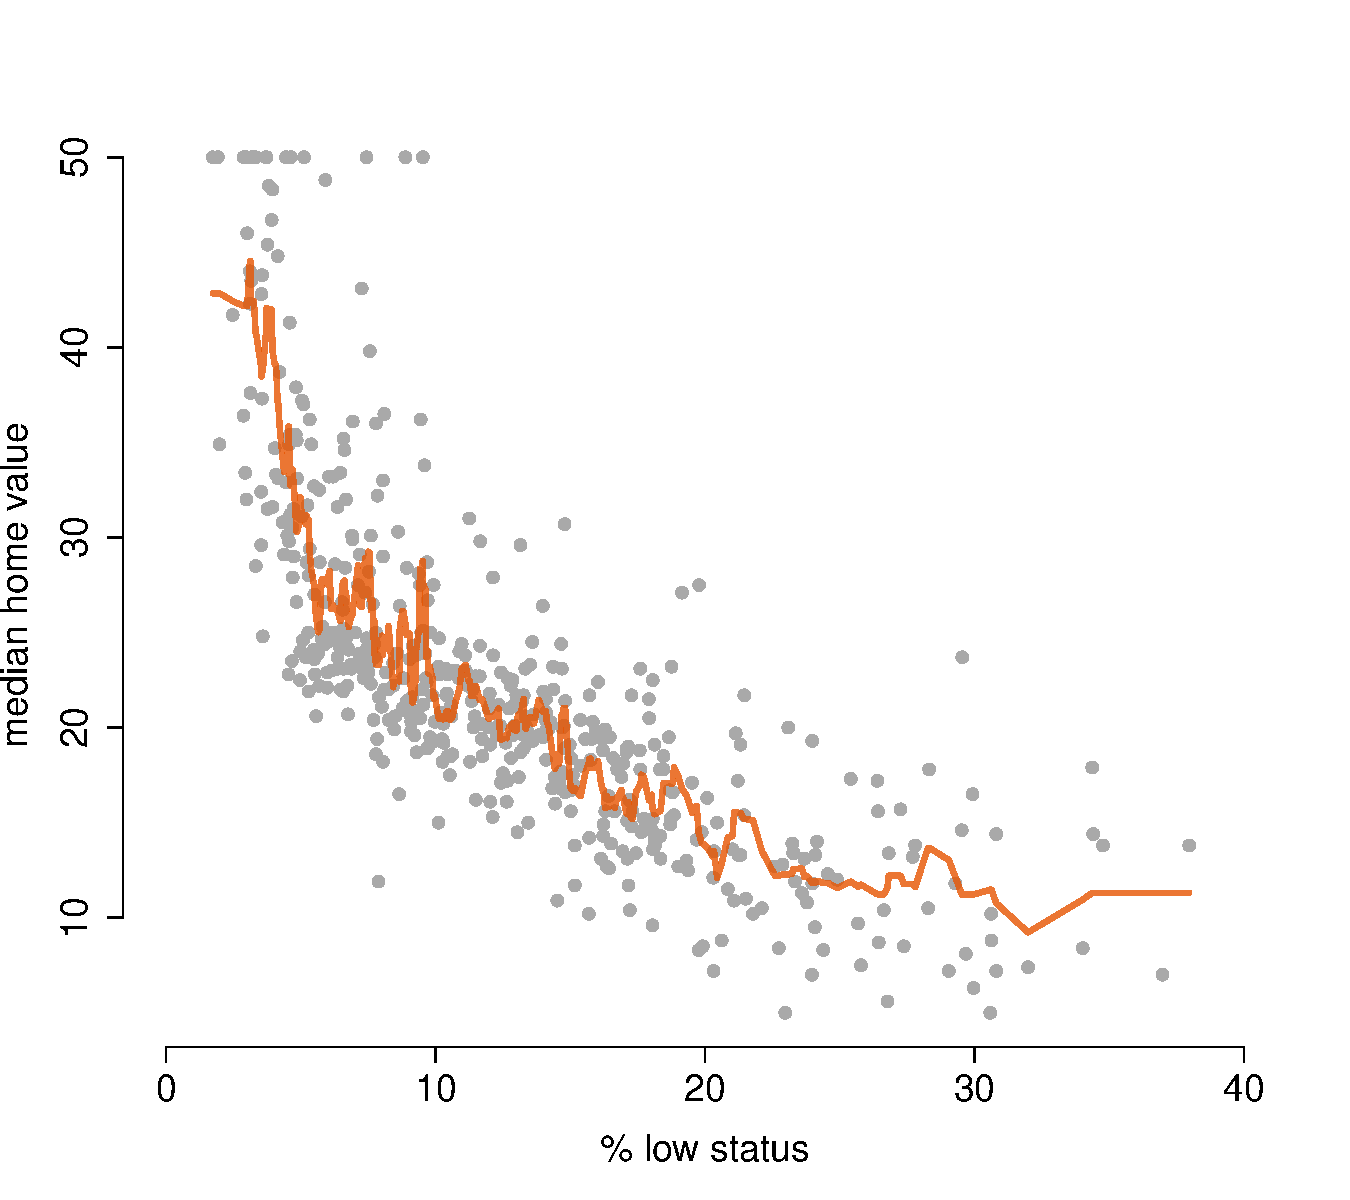
\includegraphics[scale=.44]{DaveBostonplotk=10i=2.pdf}
\end{center}
\end{frame}

\begin{frame}[plain]
\frametitle{or $\bo{k=50}$ ...}
\vspace{-8mm}
\begin{center}
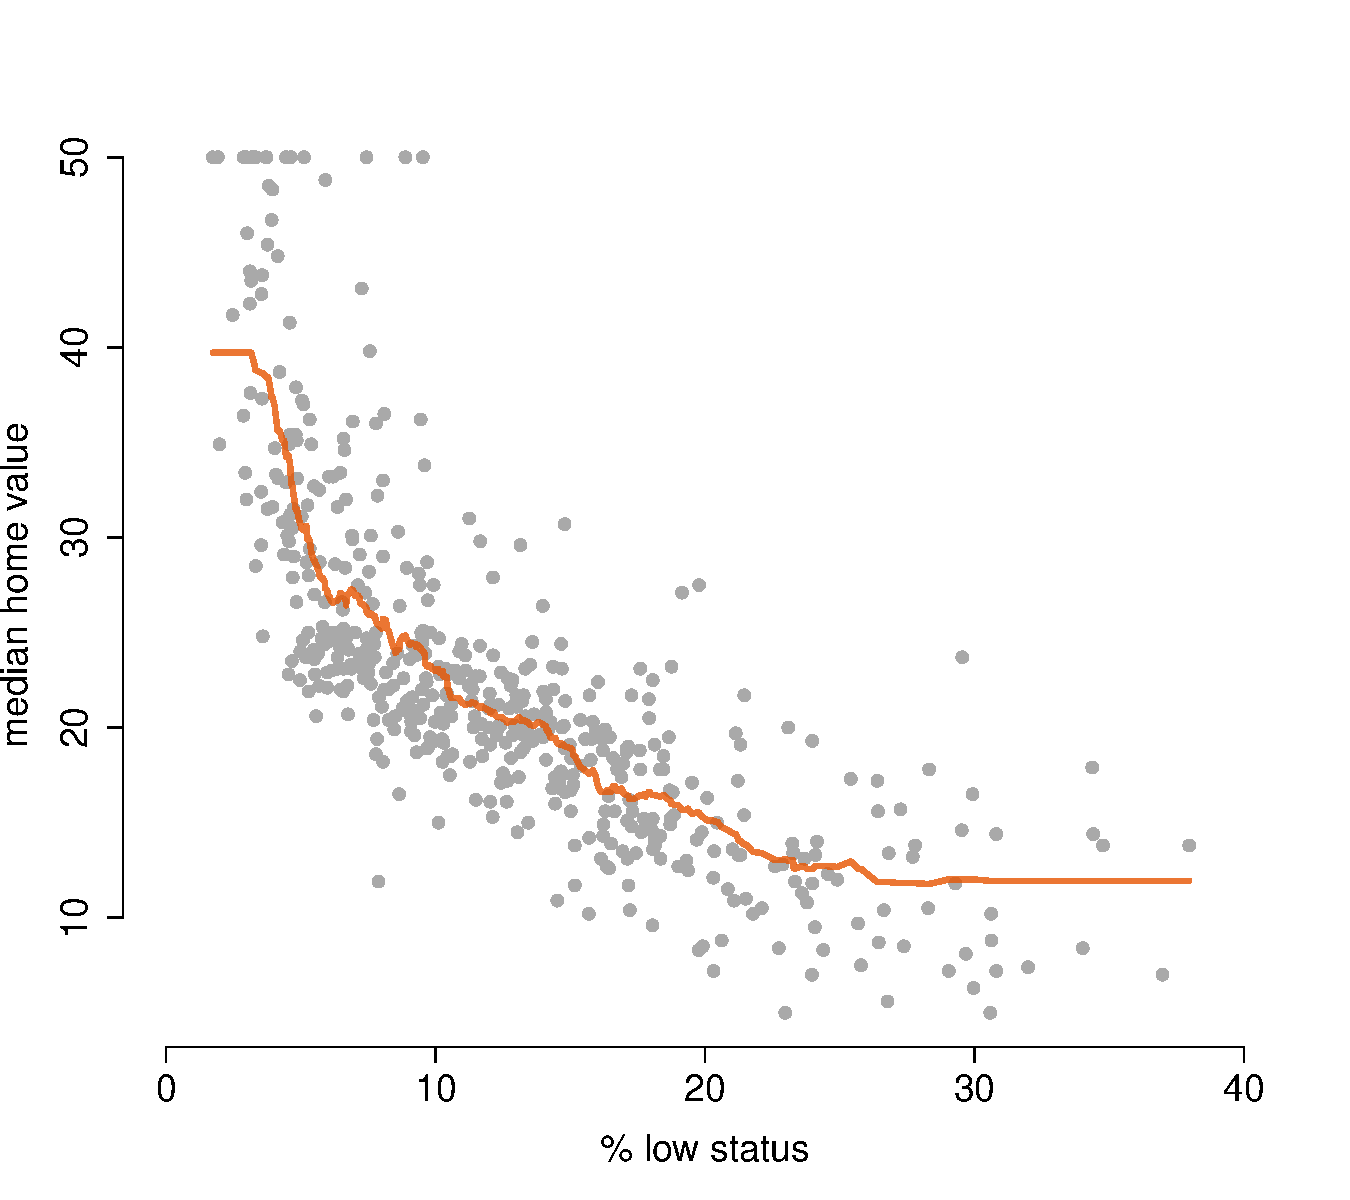
\includegraphics[scale=.44]{DaveBostonplotk=50i=3.pdf}
\end{center}
\end{frame}


\begin{frame}[plain]
\frametitle{or $\bo{k=100}$ ...}
\vspace{-8mm}
\begin{center}
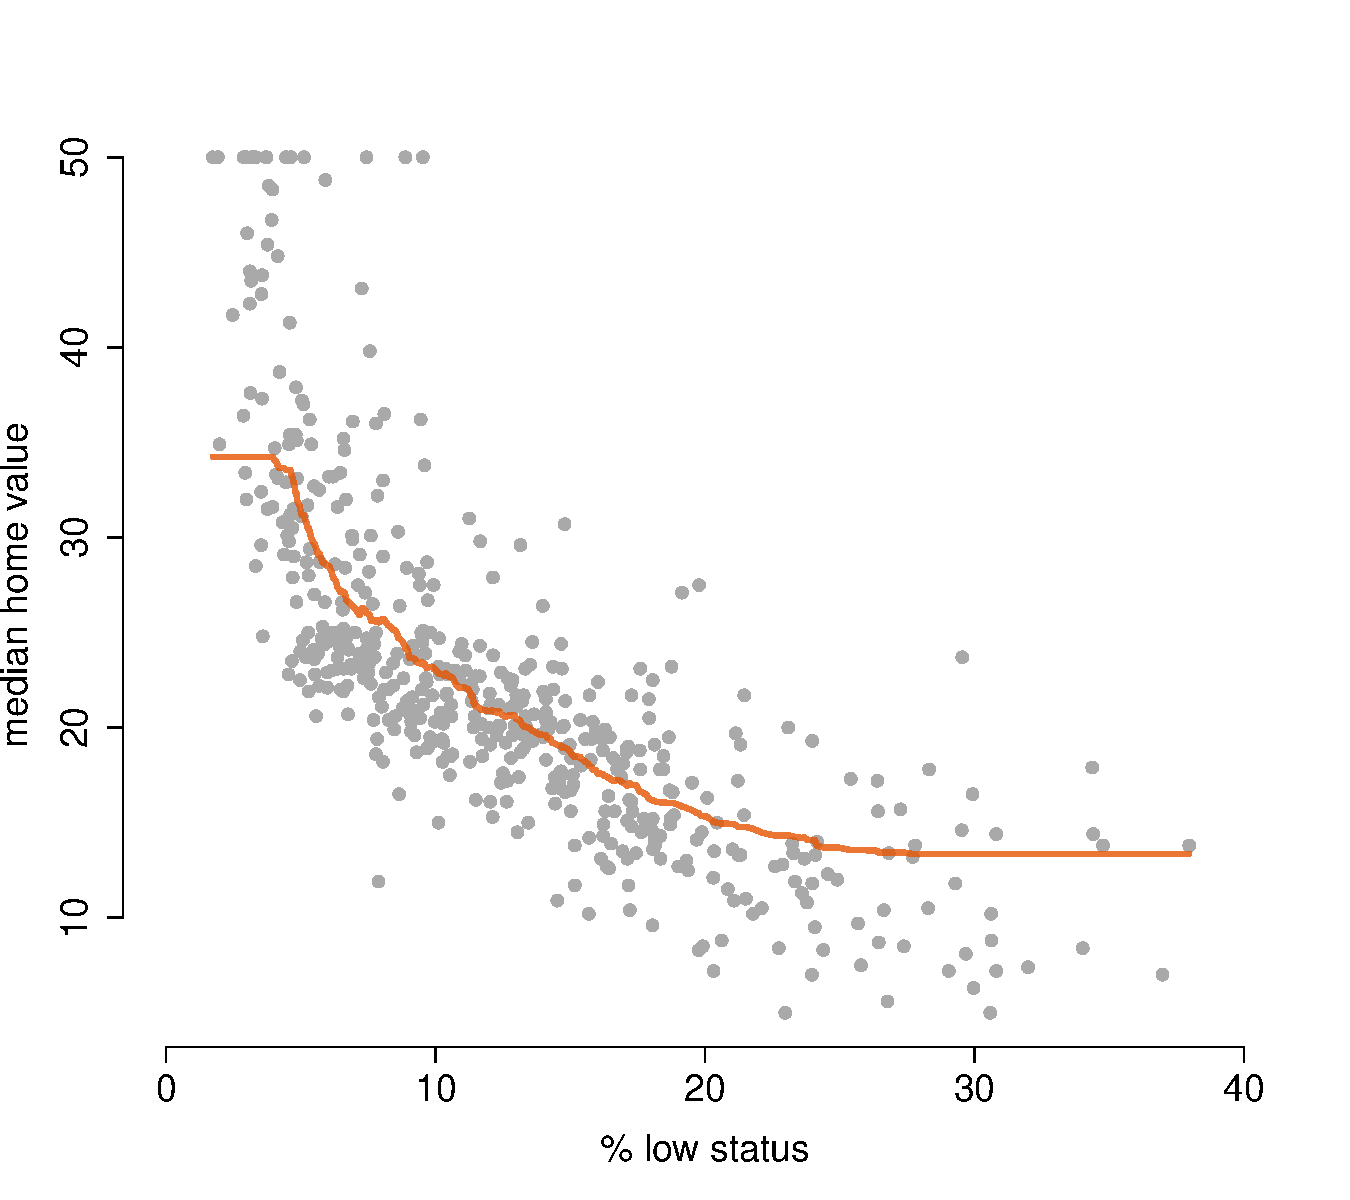
\includegraphics[scale=.44]{DaveBostonplotk=100i=4.pdf}
\end{center}
\end{frame}

\begin{frame}[plain]
\frametitle{or $\bo{k=150}$ ...}
\vspace{-8mm}
\begin{center}
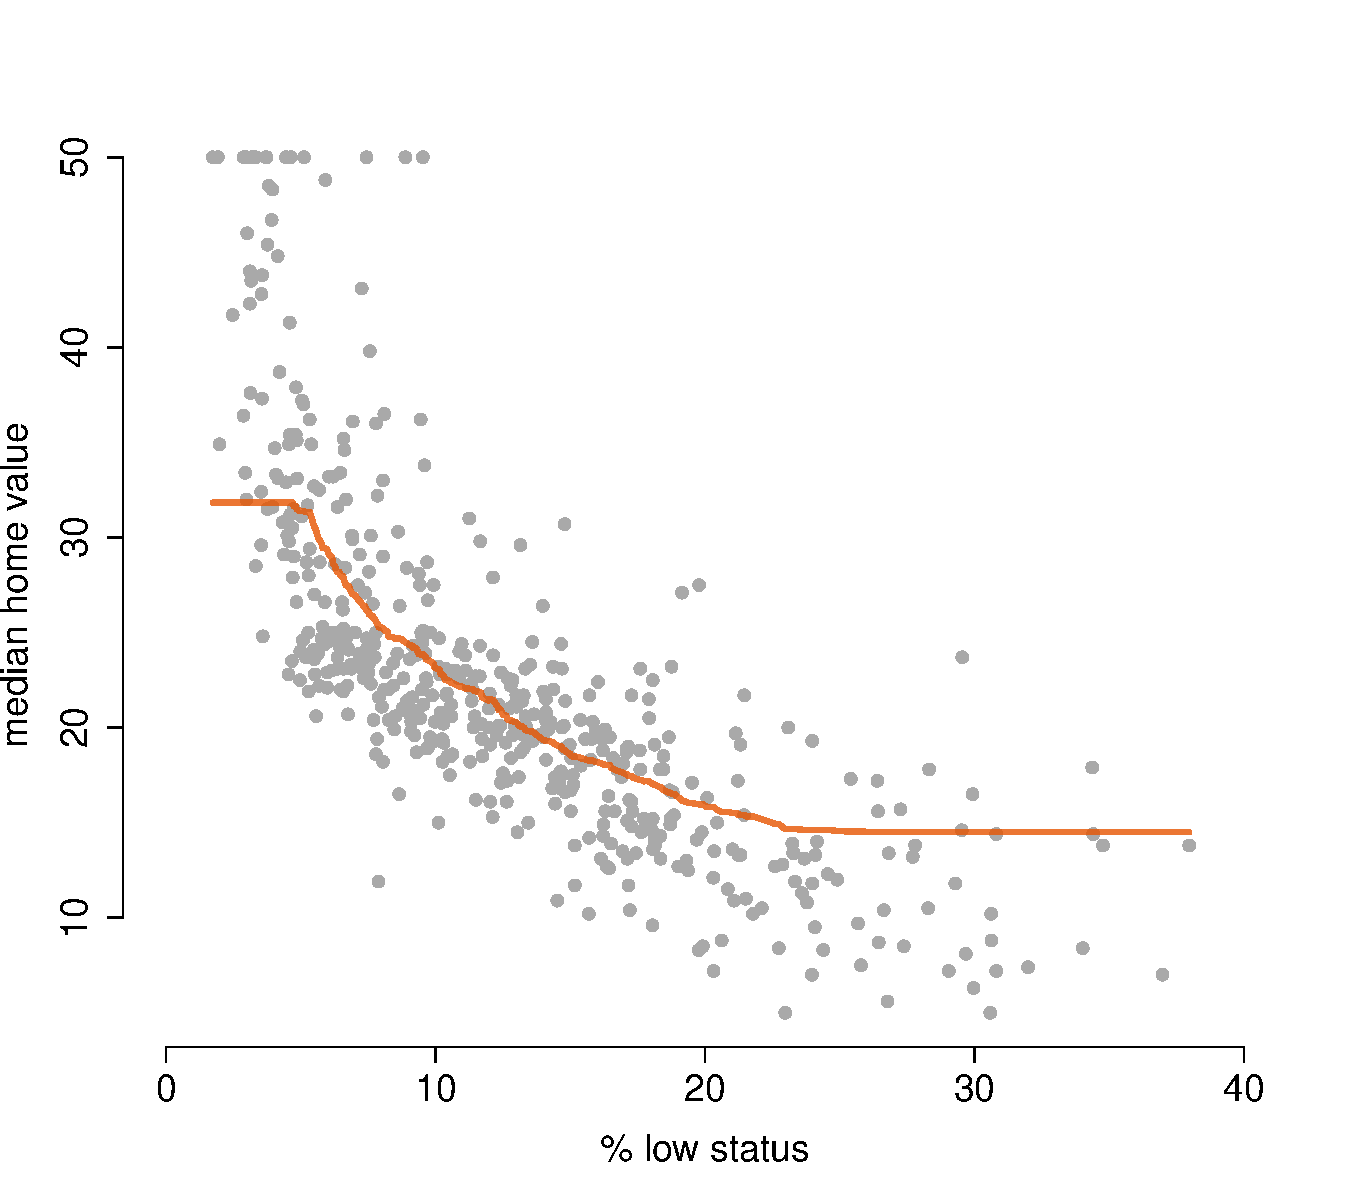
\includegraphics[scale=.44]{DaveBostonplotk=150i=5.pdf}
\end{center}
\end{frame}

\begin{frame}[plain]
\frametitle{or $\bo{k=200}$ ...}
\vspace{-8mm}
\begin{center}
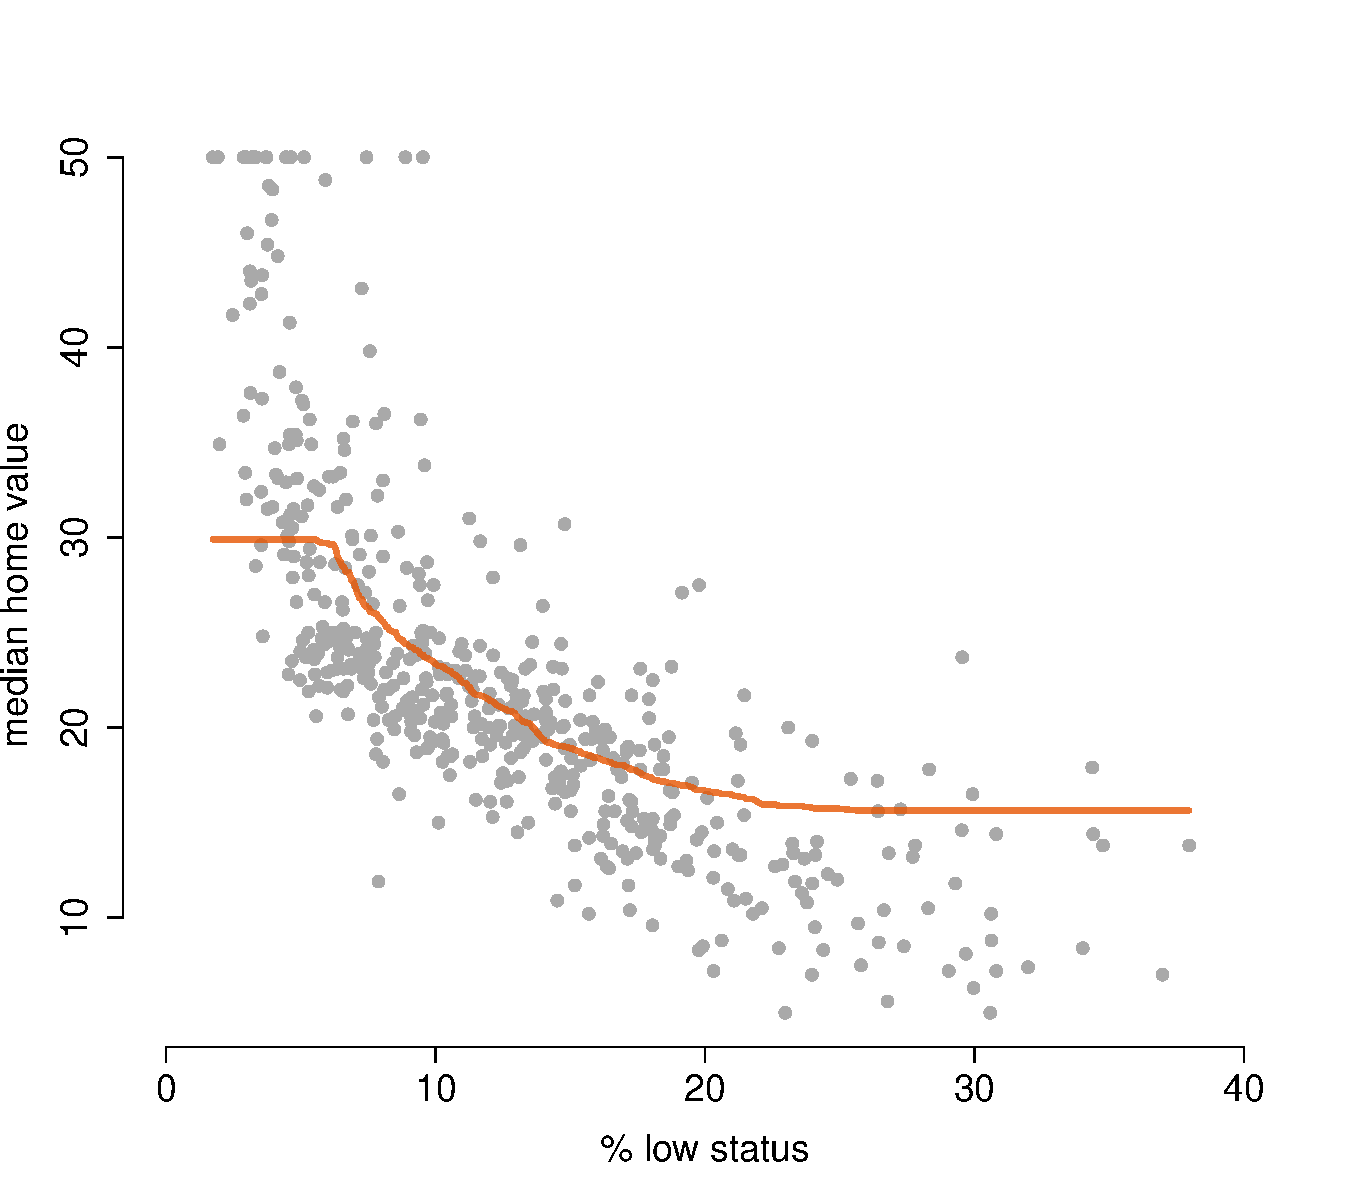
\includegraphics[scale=.44]{DaveBostonplotk=200i=6.pdf}
\end{center}
\end{frame}

\begin{frame}[plain]
\frametitle{or $\bo{k=250}$ ...}
\vspace{-8mm}
\begin{center}
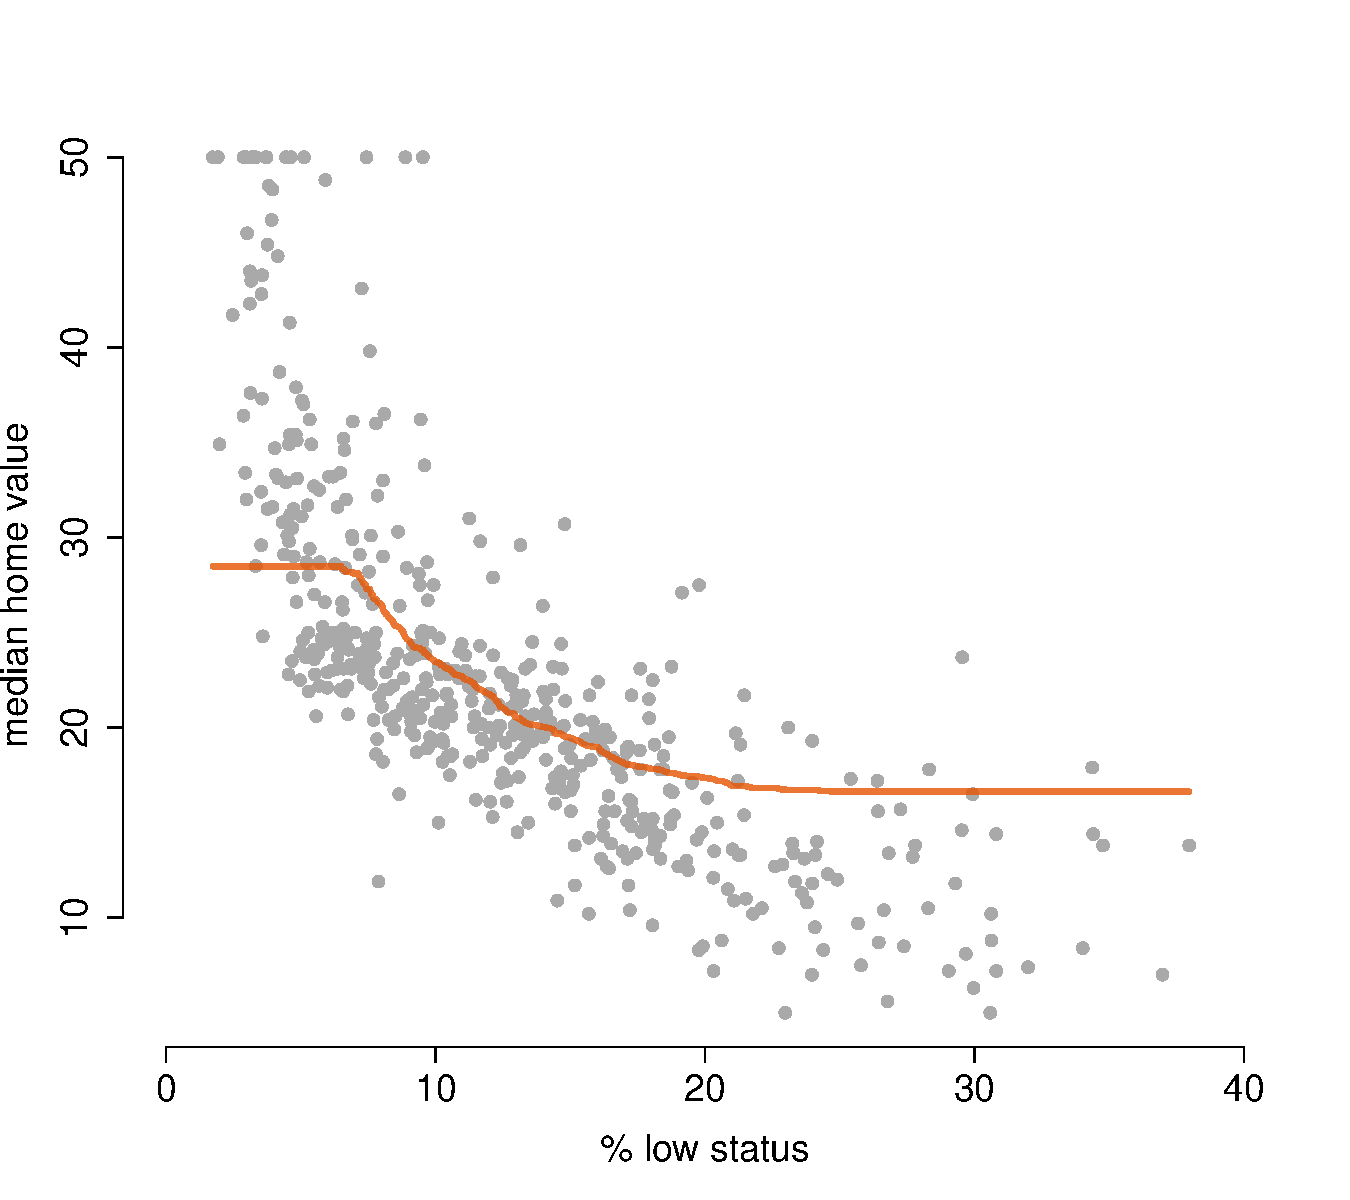
\includegraphics[scale=.44]{DaveBostonplotk=250i=7.pdf}
\end{center}
\end{frame}

\begin{frame}[plain]
\frametitle{Or $\bo{k=300}$ ...}
\vspace{-8mm}
\begin{center}
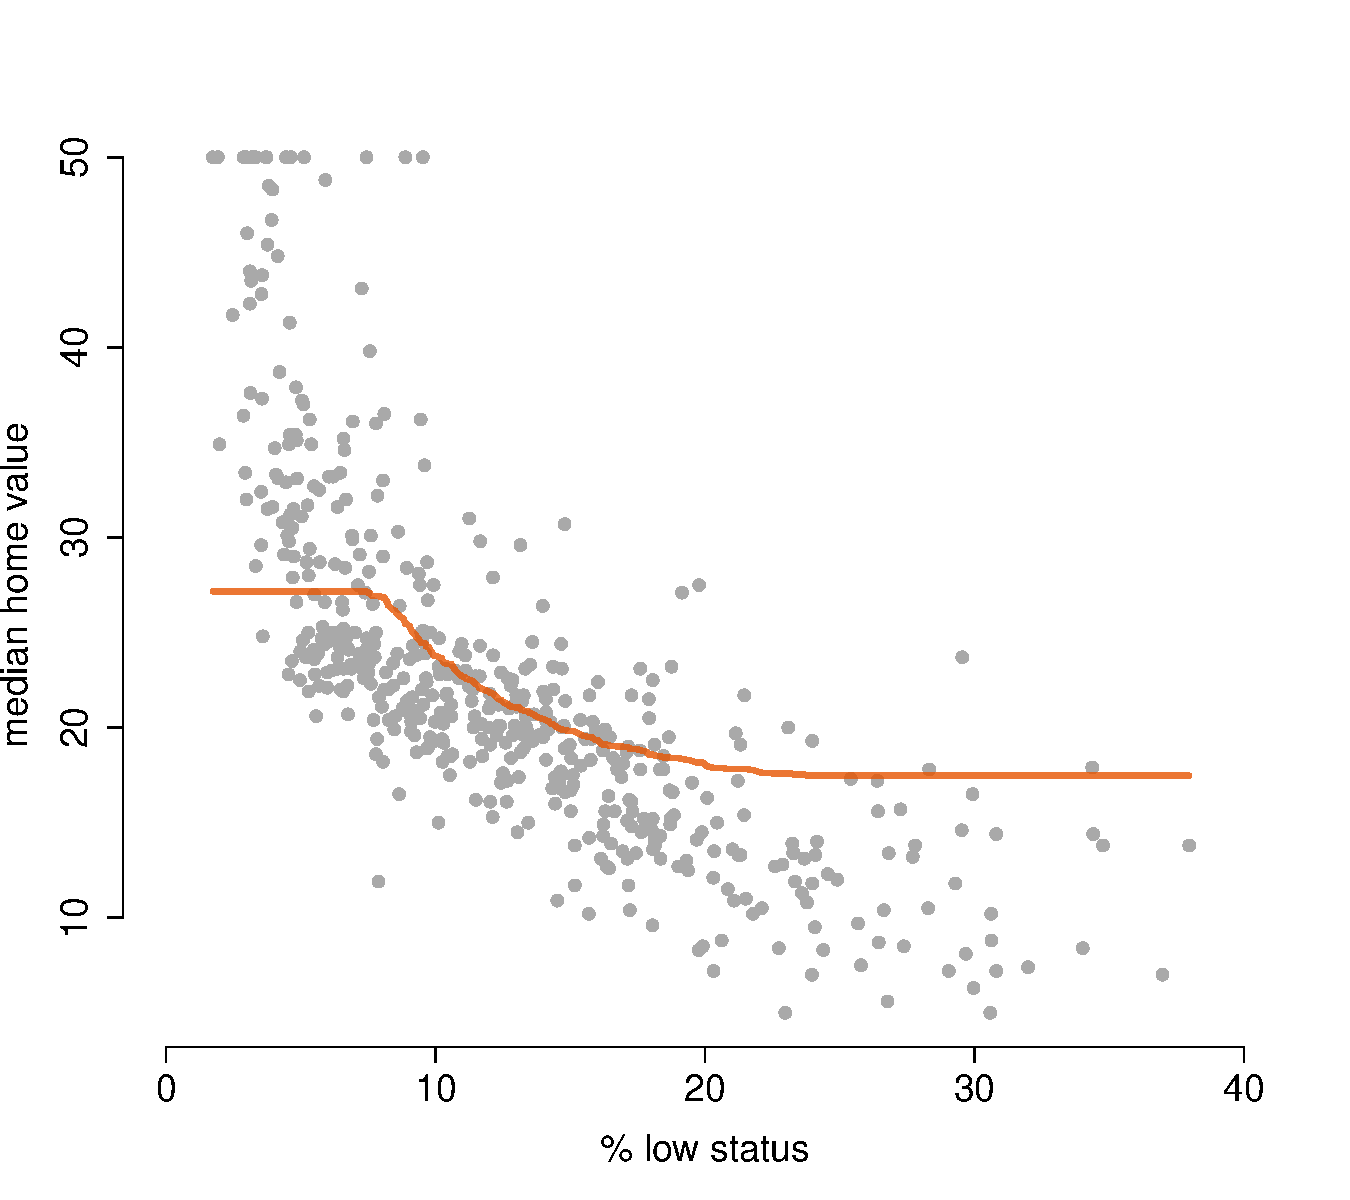
\includegraphics[scale=.44]{DaveBostonplotk=300i=8.pdf}
\end{center}
\end{frame}

\begin{frame}[plain]
\frametitle{or $\bo{k=400}$ ...}
\vspace{-8mm}
\begin{center}
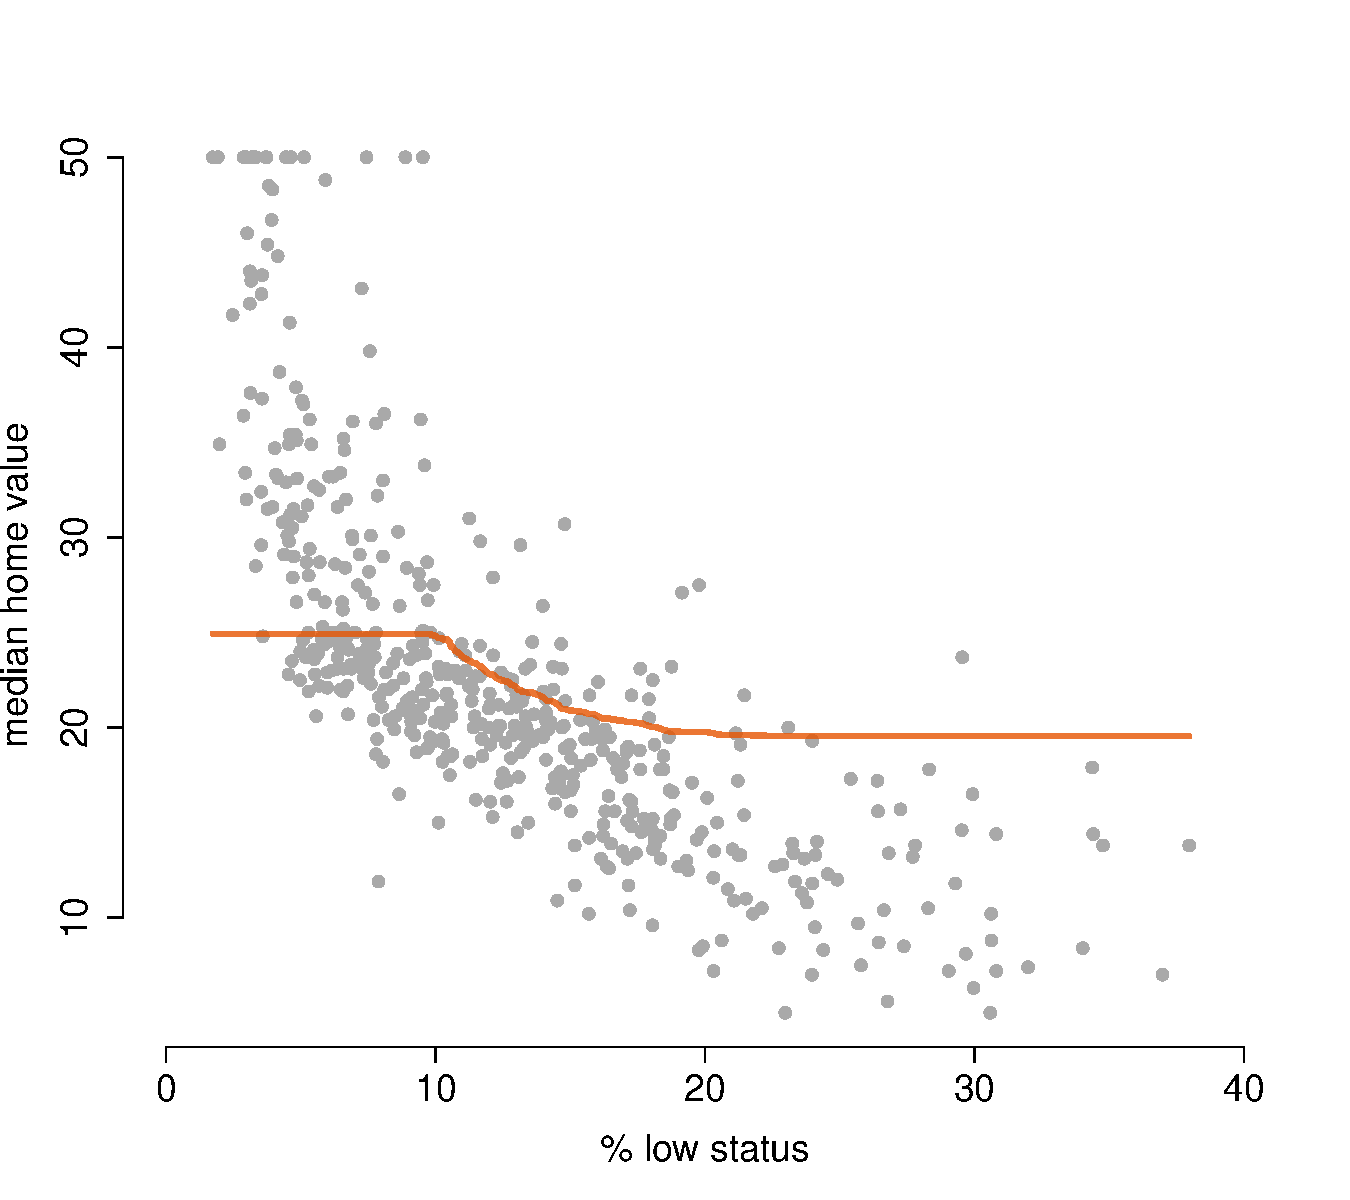
\includegraphics[scale=.44]{DaveBostonplotk=400i=9.pdf}
\end{center}
\end{frame}

\begin{frame}[plain]
\frametitle{or $\bo{k=505}$ ...}
\vspace{-8mm}
\begin{center}
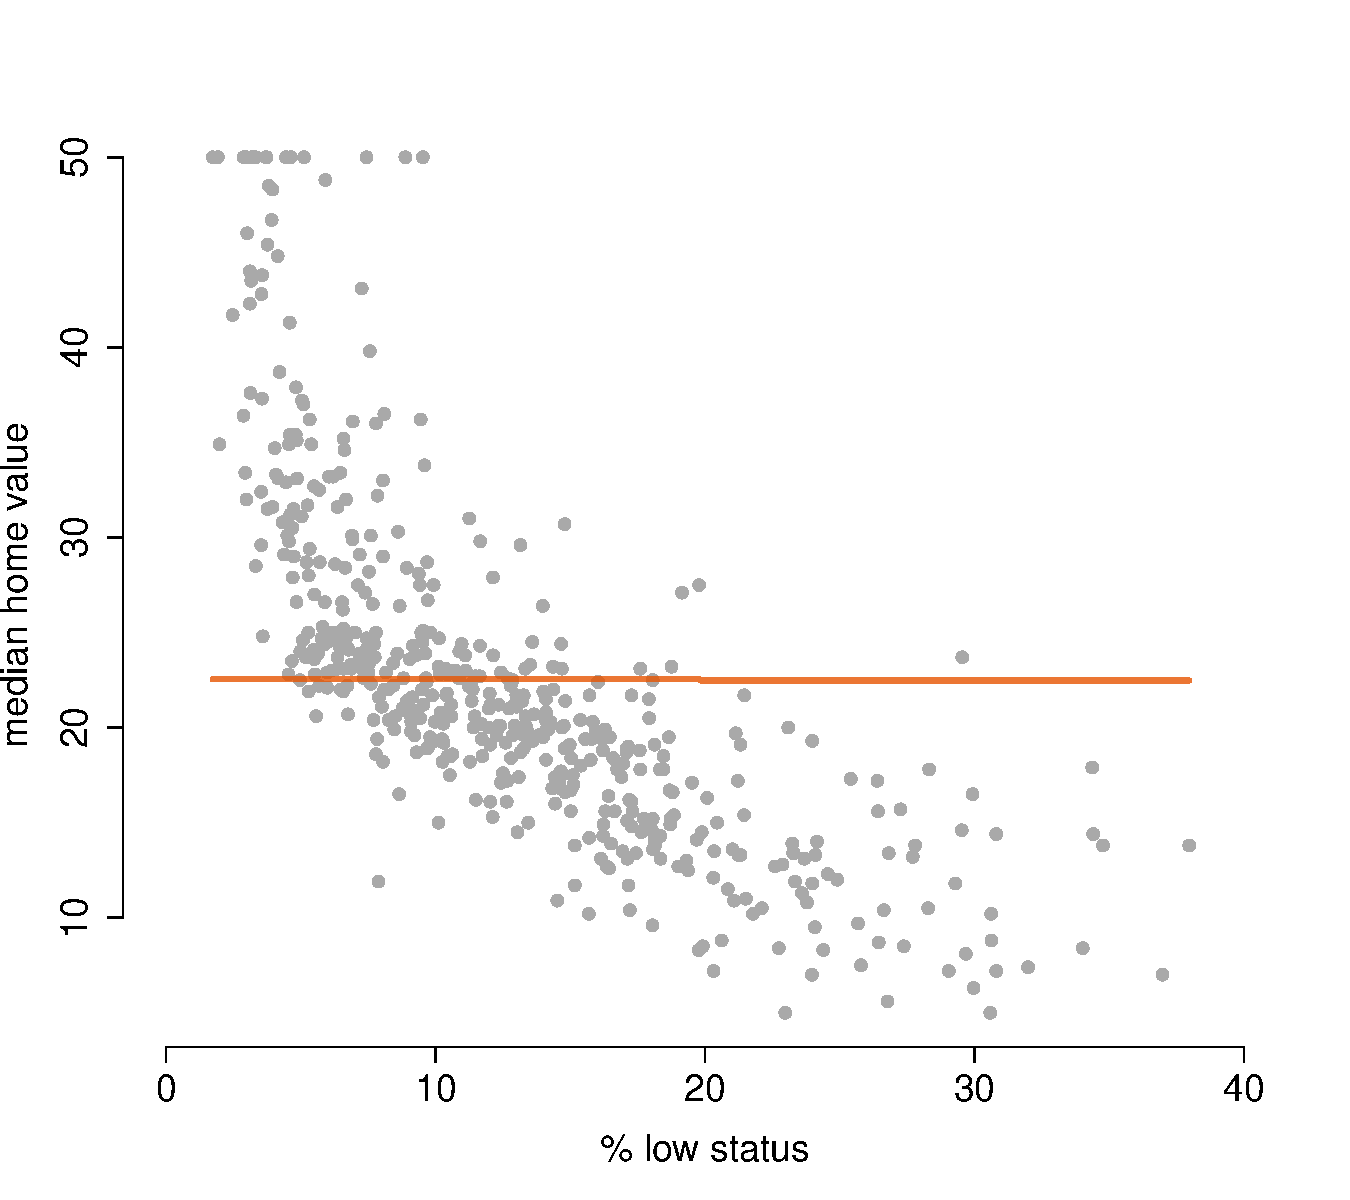
\includegraphics[scale=.44]{DaveBostonplotk=505i=10.pdf}
\end{center}
\end{frame}

\begin{frame}[plain]
\frametitle{A rigorous way to select}
\begin{itemize}
	\item The \bo{root mean squared error} measures how accurate my predictions are, on average.
\end{itemize}
\vspace{15mm}
$$
RMSE = \sqrt{\frac{1}{n} \sum_{i=1}^n \left[Y_i - \widehat{f(X_i})\right]^2}
$$

\end{frame}

\begin{frame}[plain]
\frametitle{In sample RMSE}
\vspace{5mm}
\begin{itemize}
\item[] It looks like \bo{$k=2$} is the best. Should we choose this model?
\end{itemize}
\vspace{-9mm}
\begin{center}
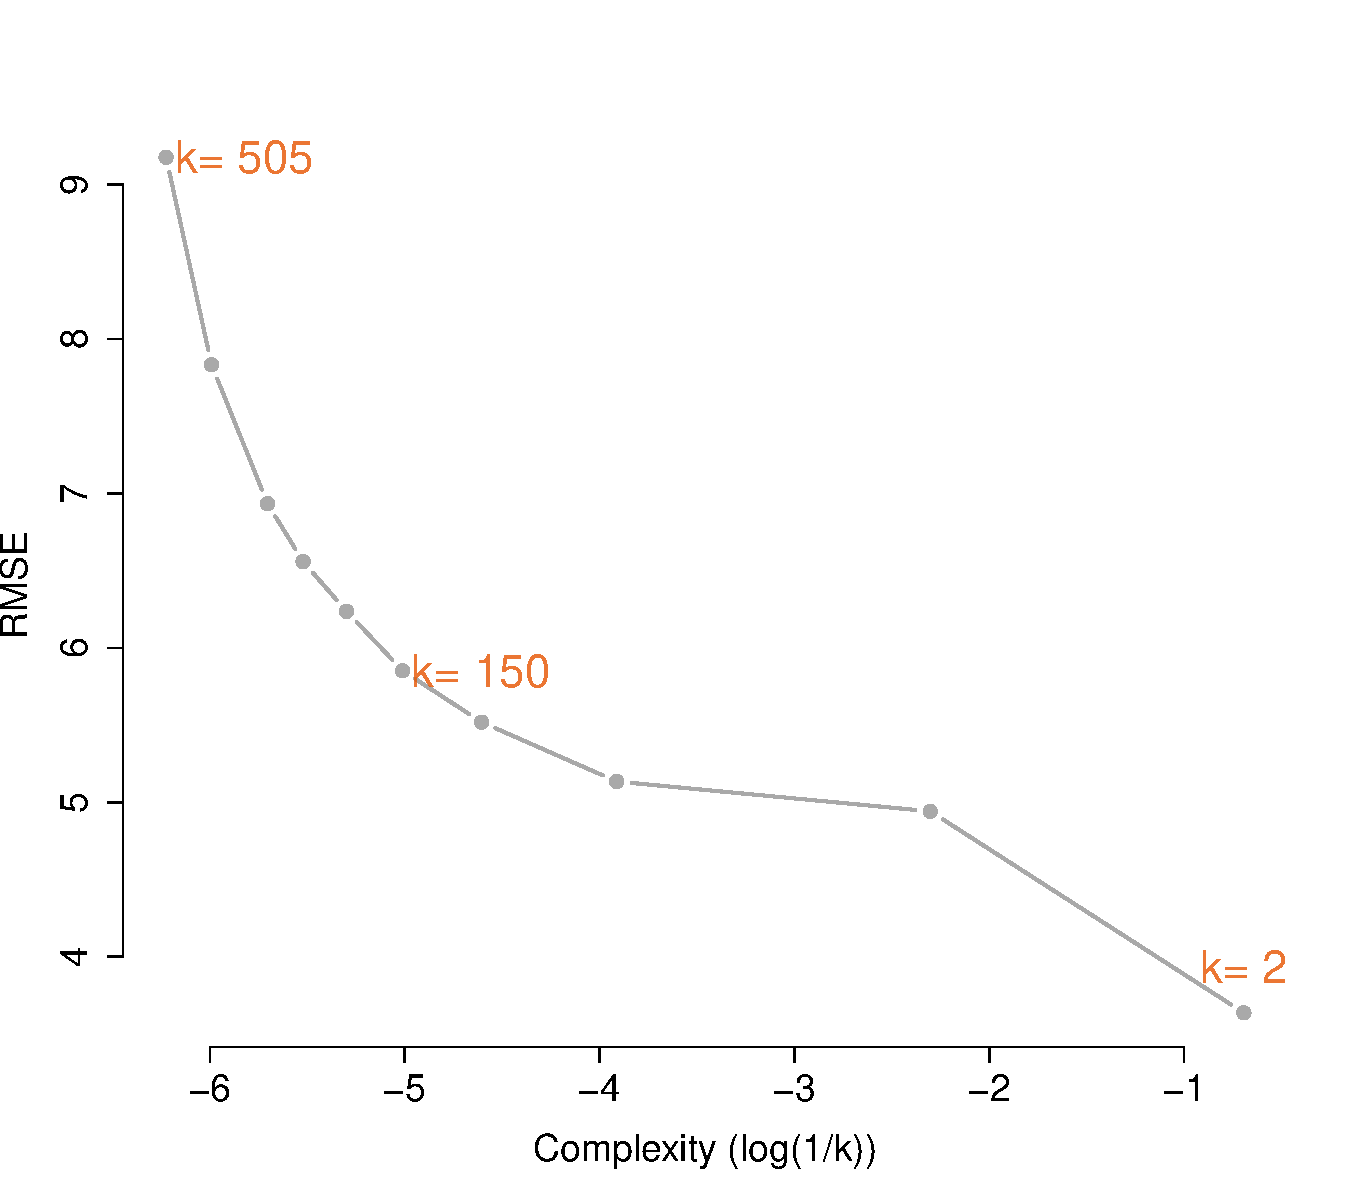
\includegraphics[scale=.39]{DaveBostonplotINMSE.pdf}
\end{center}
\end{frame}

\begin{frame}[plain]
\frametitle{We care about \bo{out of sample} performance}
\vspace{5mm}
\begin{itemize}
	\item Suppose we have $m$ additional observations  $(X^o_i,Y^o_i)$, for $i=1,\dots,m$, \bo{that we did not use to fit the model}. Let's call this dataset the \bo{{\it validation set} }(a.k.a {\it hold-out set} or {\it test set})\vspace{9mm}\pause
	\item We evaluate the fit with \bo{out of sample} RMSE:
\end{itemize}
\vspace{8mm}
$$
RMSE^o = \sqrt{\frac{1}{m} \sum_{i=1}^m \left[Y^o_i - \widehat{f(X^o_i})\right]^2}
$$
\end{frame}

\begin{frame}[plain]
\frametitle{Out of sample RMSE}
\vspace{4mm}

Fit each model on training set of size \bo{400}. Test each model ({\it out of sample}) on testing set of size \bo{106}.  Here, we plot the out of sample performance.   

\vspace{-12mm}
\begin{center}
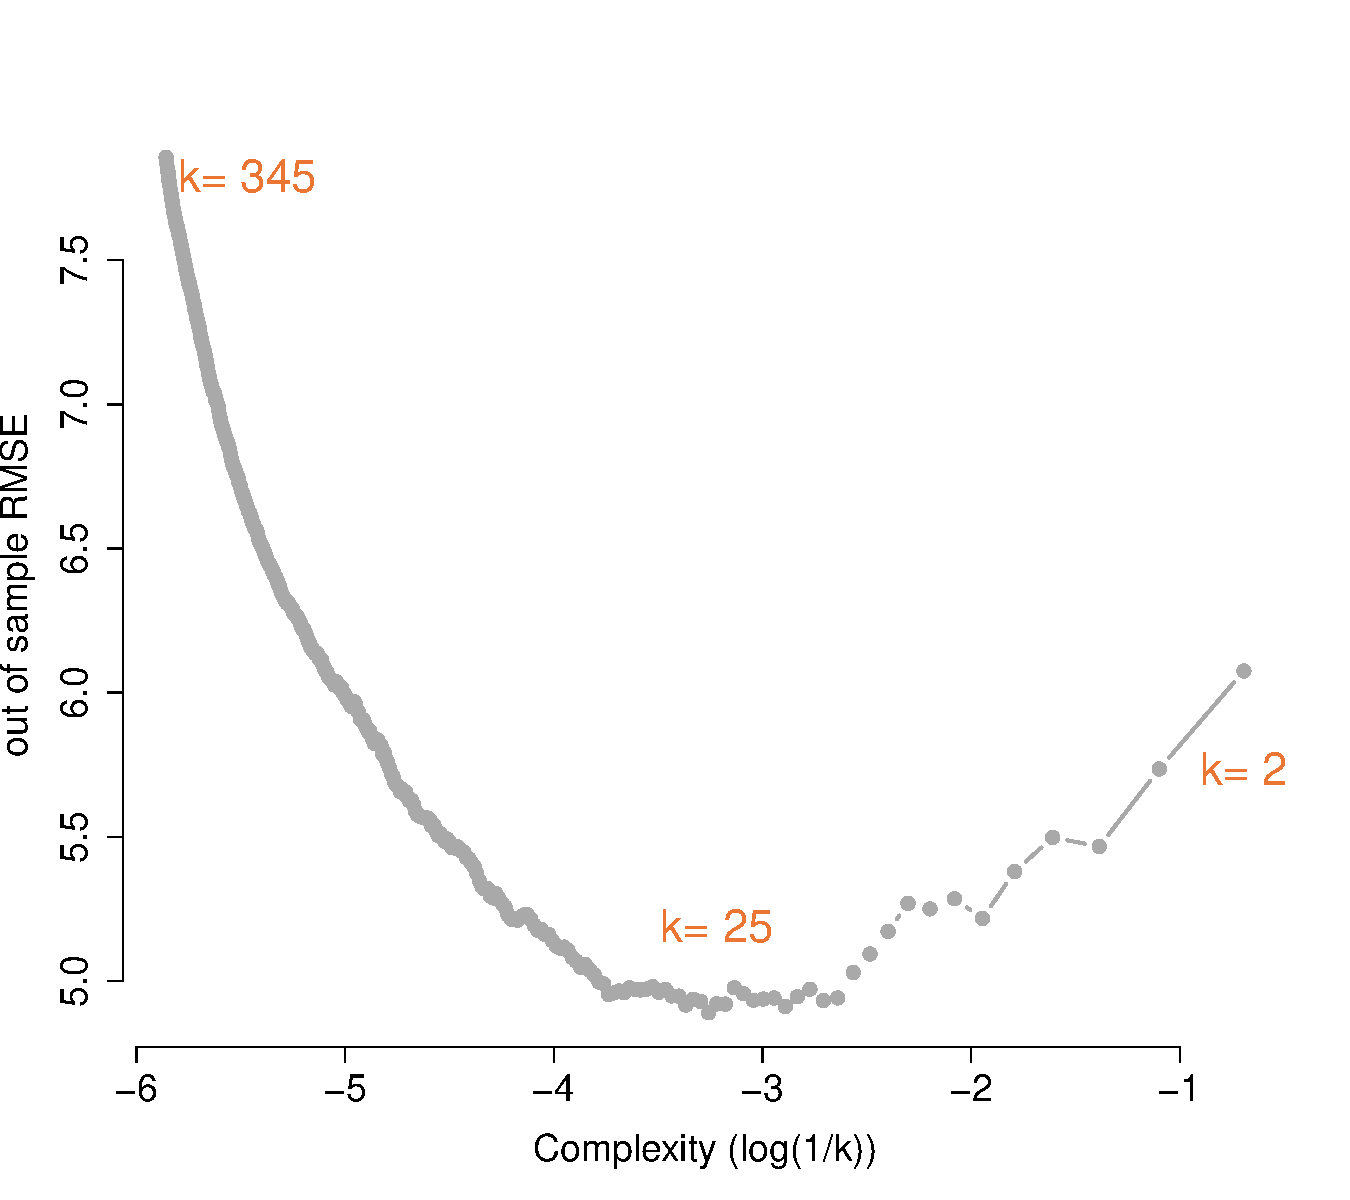
\includegraphics[scale=.39]{DaveBostonplotOUTMSE.pdf}
\end{center}
\end{frame}

\begin{frame}[plain]
\frametitle{The Bias-variance tradeoff!}
\vspace{4mm}
When fitting a predictive model, there is a tradeoff between \bo{bias} and \bo{variance} of predictions.  
\vspace{5mm}
\begin{center}
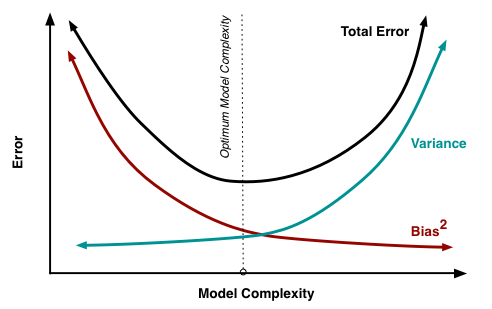
\includegraphics[scale=.5]{biasvariance}
\end{center}
\end{frame}

\begin{frame}[plain]
\frametitle{$\bo{k=2}$: low bias, high variance}
\vspace{4mm}
Training set of size 40.  
\vspace{-10mm}
\begin{center}
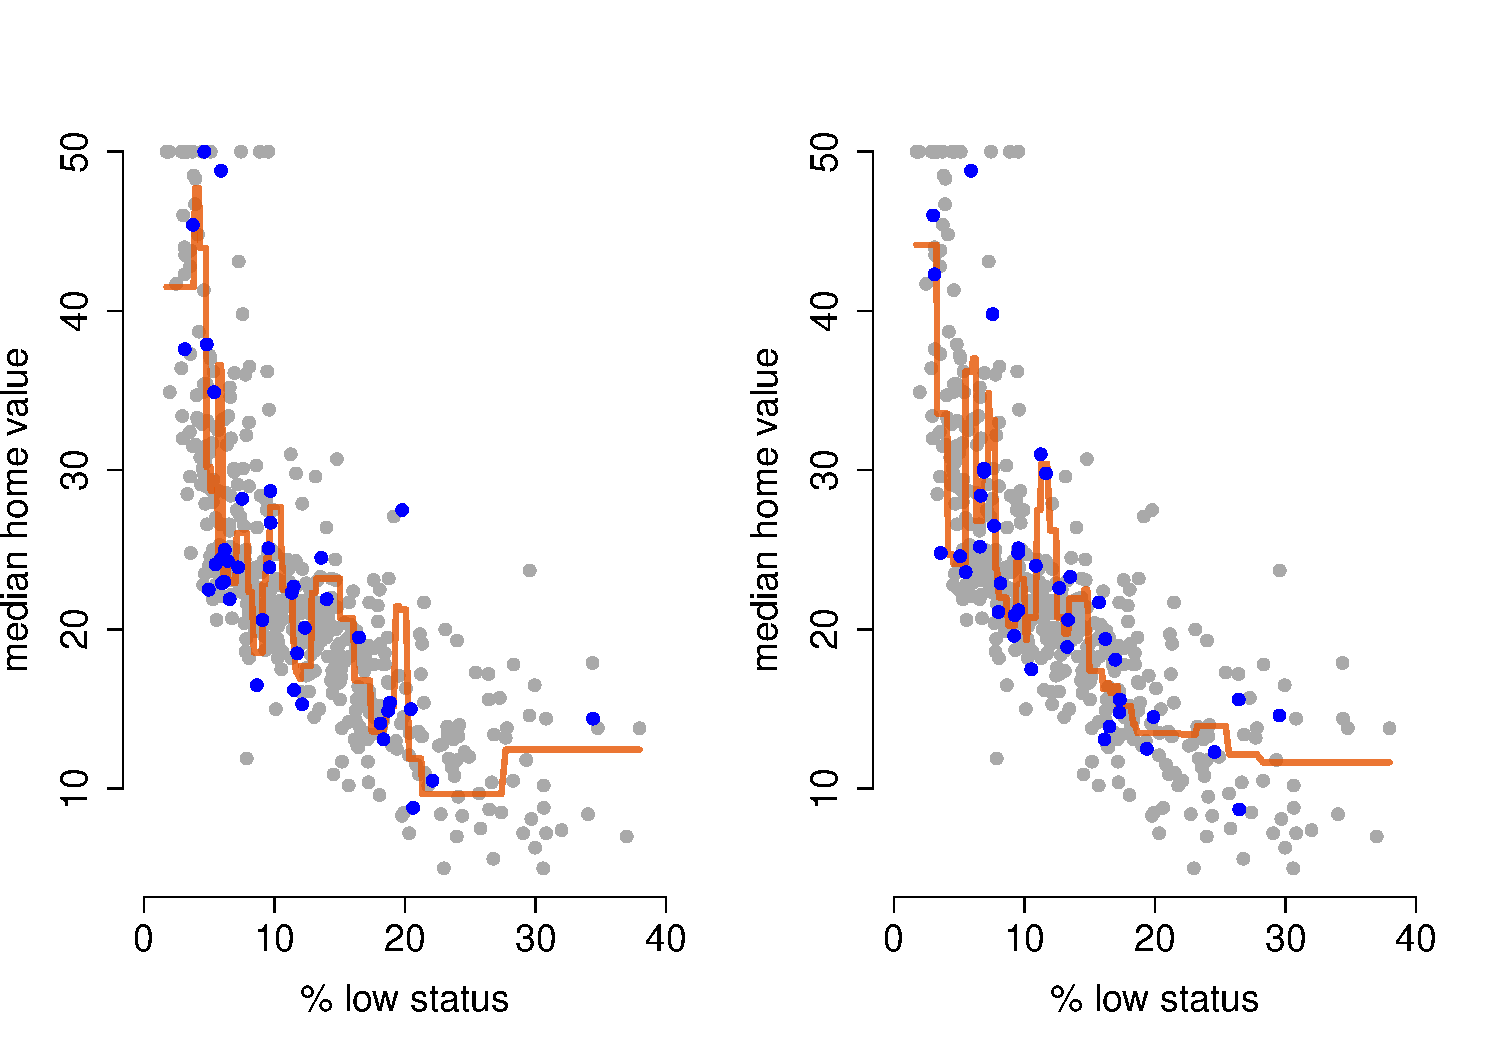
\includegraphics[scale=.43]{DaveBostonplotk2BVTrade1}
\end{center}
\end{frame}

\begin{frame}[plain]
\frametitle{$\bo{k=25}$: high bias, low variance}
\vspace{4mm}
Training set of size 40.
\vspace{-10mm}
\begin{center}
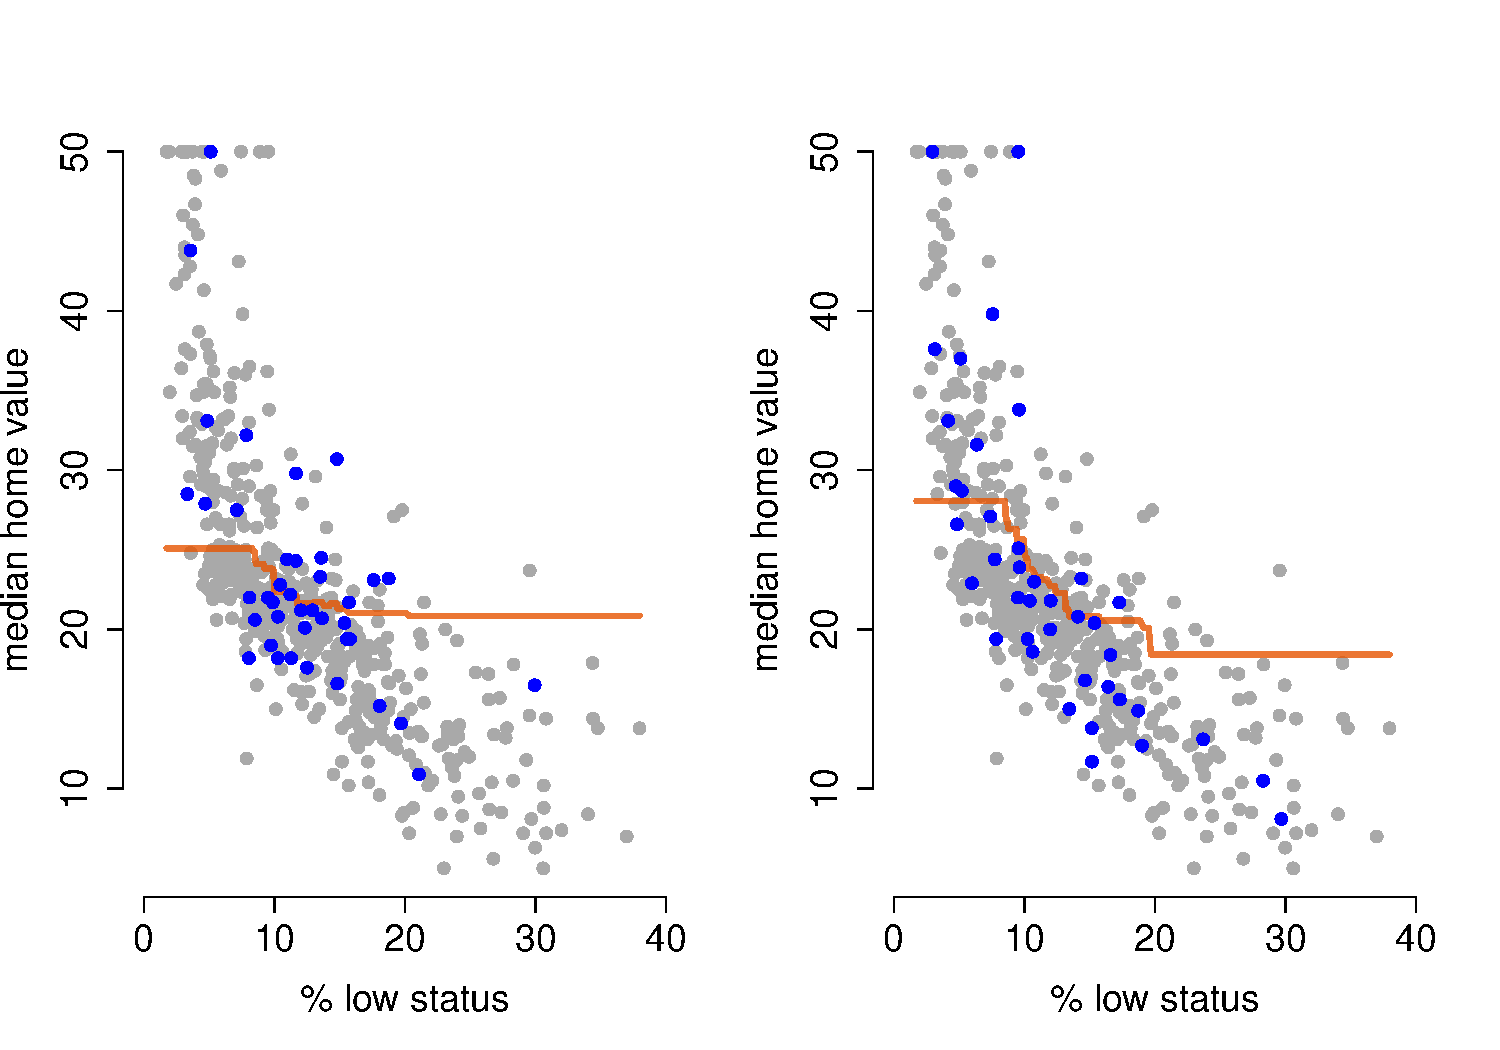
\includegraphics[scale=.43]{DaveBostonplotk25BVTrade1}
\end{center}
\end{frame}


%\begin{frame}
%	\frametitle{Relationship to linear regression}
%	
%	Selecting $k$ is Knn is the same as selecting which variables to include in your regression model! \\ \sk 
%	
%	In both cases, you are trying to build the \bo{best model} for your outcome $Y$. \\ \sk
%	
%	\dg{Questions that remain unanswered}: \\ \sko
%	\ba How does model selection relate to causal inference? \\ \sko
%	\ba More directly, how can we use the best ideas from machine learning to help us automatically \lb{\bf control for} the variables we need in our model?
%\end{frame}
%
%\begin{frame}
%	\frametitle{Where we're headed next}
%	
%	
%\dg{First}, we will overview model selection methods for linear regression. \\ \sk \dg{Second}, we will discuss tree-based modeling (and the implicit selection that goes on), one of the most popular nonlinear modeling techniques available.
%
%\sk\sk
%
%In both cases, the goal is to include all measured covariates in the model and let the statistical method \bo{select} which ones are the most important.
%
%\end{frame}
%
%
%\begin{frame}
%
%\sk\sk
%\dg{\Large \bf Linear models and the B-V tradeoff}
%\end{frame}
%
%\begin{frame}
%\frametitle{Variable selection and regularization} 
%When working with linear regression models where the number of $X$ variables is large, we need to think about strategies to {\color{lightblue}select what variables to use...}
%
%\skoo
%
%We will focus on 2 ideas:
%\begin{itemize} 
%\sko
%\item Subset Selection
%\item Shrinkage
%\end{itemize}
%\end{frame}
%
%
%%%%%%%%%%%%%%%%%%%%%%%%%%%%%%%%%%%%%%%
%\begin{frame}
%\frametitle{Subset selection}
%
%The idea here is very simple: {\color{lightblue}fit as many models as you can and compare their performance based on some criteria!}
%
%\skoo
%
%Issues:
%\begin{itemize} \sk
%\item How many possible models? Total number of models = $2^p$ \\ {\color{red}Is this large?}
%\item What criteria to use? \\
%{\color{red}Just as before, if prediction is what we have in mind, out-of-sample predictive ability should be the criteria}
%\end{itemize}
%
%
%\end{frame}
%
%%%%%%%%%%%%%%%%%%%%%%%%%%%%%%%%%%%%
%\begin{frame}
%\frametitle{Information criteria}  \vskip -.25cm
%
%Another way to evaluate a model is to use   \bl Information Criteria \bk metrics
%which attempt to quantify how well our model \rd would \bk have
%predicted the data (regardless of what you've estimated for the
%$\beta_j$'s).
%
%\sk
%A good alternative is the \bl BIC: Bayes Information Criterion\bk,
%which is based on a ``Bayesian''  philosophy of statistics.\\
%\vskip -.2cm
%{\Large \[  BIC = n\log(s^2) + p\log(n) \]}
%\vskip -.25cm
%You want to choose the model that leads to \bl minimum \bk BIC.
%
%\end{frame}
%
%%%%%%%%%%%%%%%%%%%%%%%%%%%%%%%%%%%%
%\begin{frame}
%\frametitle{Information criteria}  \vskip -.25cm
%
%
%One nice thing about the BIC is that you can
%interpret it in terms of
%\bl model probabilities\bk.  
%
%\sko
% Given a list of  possible models $\{M_1, M_2,\ldots,M_R\}$, the probability that
%model $i$ is correct is
%\vskip -.25cm
%{\large
%\begin{eqnarray*}
%P(M_i) \approx \frac{e^{-\frac{1}{2}BIC(M_i)} }{\sum_{r=1}^R
%  e^{-\frac{1}{2}BIC(M_r)}}
%=\frac{e^{-\frac{1}{2}[BIC(M_i){\bl-BIC_{min}}]} }{\sum_{r=1}^R
%  e^{-\frac{1}{2}[BIC(M_r){\bl-BIC_{min}}]}}
%\end{eqnarray*} }
%
%{\footnotesize (Subtract $BIC_{min} = \min\{BIC(M_1)\ldots BIC(M_R)\}$
%  for numerical stability.) }
%
%\skoo
%
%Similar, alternative criteria include AIC, $C_p$, adjusted $R^2$... \\ \sko{\color{lightblue} {\bf Bottom line}: these are only useful if we lack the ability to compare models based on their out-of-sample predictive ability!}
%
%
%
%\end{frame}
%
%
%
%%%%%%%%%%%%%%%%%%%%%%%%%%%%%%%%%%%%%%%
%\begin{frame}
%\frametitle{Search strategies: Stepwise regression}
%One computational approach to build a regression model step-by-step is ``stepwise regression''  There are 3 options:
%\bi \sk
%\item {\color{red} Forward:} adds one variable at the time until no remaining variable makes a significant contribution (or meet a certain criteria... could be out of sample prediction)
%\item {\color{red} Backwards:} starts will all possible variables and removes one at the time until further deletions would do more harm them good
%\item {\color{red} Stepwise:} just like the forward procedure but allows for deletions at each step
%\ib 
%
%\end{frame}
%
%
%%%%%%%%%%%%%%%%%%%%%%%%%%%%%%%%%%%%%%%
%\begin{frame}
%\frametitle{Shrinkage methods}
%
%An alternative way to deal with selection is to \bo{\bf work with all $p$ predictors at once} while placing a constraint on the size of the estimated coefficients
%
%\skoo
%
%This idea is a regularization technique that reduces the variability of the estimates and tend to lead to better predictions. 
%
%\skoo
%
%The hope is that by having the constraint in place, the estimation procedure will be able to focus on ``the important $\beta$'s''
%
%\end{frame}
%
%%%%%%%%%%%%%%%%%%%%%%%%%%%%%%%%%%%%%%%
%\begin{frame}
%\frametitle{Ridge regression}
%{\color{lightblue} Ridge regression} is a modification of the least squares criteria that minimizes (as a function of $\beta$'s)\sko
%$$
%{\color{lightblue}\sum_{i=1}^n \left( Y_i - \beta_0 -  \sum_{j=1}^p \beta_j X_{ij} \right)^2 }+ {\color{red}\lambda\sum_{j=1}^p \beta_j^2}  
%$$
%
%\sko
%for some value of $\lambda >0$ 
%
%\skoo
%
%\begin{itemize}
%\item The {\color{lightblue}``blue''} part of the equation is the traditional objective function of LS
%\item The {\color{red}``red''} part is the shrinkage penalty, ie, something that makes costly to have big values for $\beta$
%\end{itemize}
%\end{frame}
%
%
%%%%%%%%%%%%%%%%%%%%%%%%%%%%%%%%%%%%%%%
%\begin{frame}
%\frametitle{Ridge regression}
%$$
%{\color{lightblue}\sum_{i=1}^n \left( Y_i - \beta_0 -  \sum_{j=1}^p \beta_j X_{ij} \right)^2 }+ {\color{red}\lambda\sum_{j=1}^p \beta_j^2}  
%$$\sko
%
%\begin{itemize}
%\item if $\lambda = 0$ we are back to least squares
%\item when $\lambda \rightarrow \infty$, it is {\color{red}``too expensive''} to allow for any $\beta$ to be different than 0... 
%\item So, for different values of $\lambda$ we get a different solution to the problem
%\end{itemize}
%\end{frame}
%
%
%%%%%%%%%%%%%%%%%%%%%%%%%%%%%%%%%%%%%%%
%\begin{frame}
%\frametitle{Ridge regression}
%\begin{itemize}
%\item What ridge regression is doing is exploring the {\color{lightblue}bias-variance trade-off!} The larger the $\lambda$ the more bias (towards zero) is being introduced in the solution, ie, the less flexible the model becomes... at the same time, the solution has less {\color{red}variance}
%\item  As always, the trick to find the ``right'' value of $\lambda$ that makes the model {\color{lightblue}not too simple but not too complex!} 
%\item Whenever possible, we will choose $\lambda$ by comparing the out-of-sample performance (usually via cross-validation)
%\end{itemize}
%
%\end{frame}
%
%%%%%%%%%%%%%%%%%%%%%%%%%%%%%%%%%%%%%%%
%\begin{frame}
%\frametitle{Ridge regression}
%\vspace{-0.8cm}
%\begin{center}
%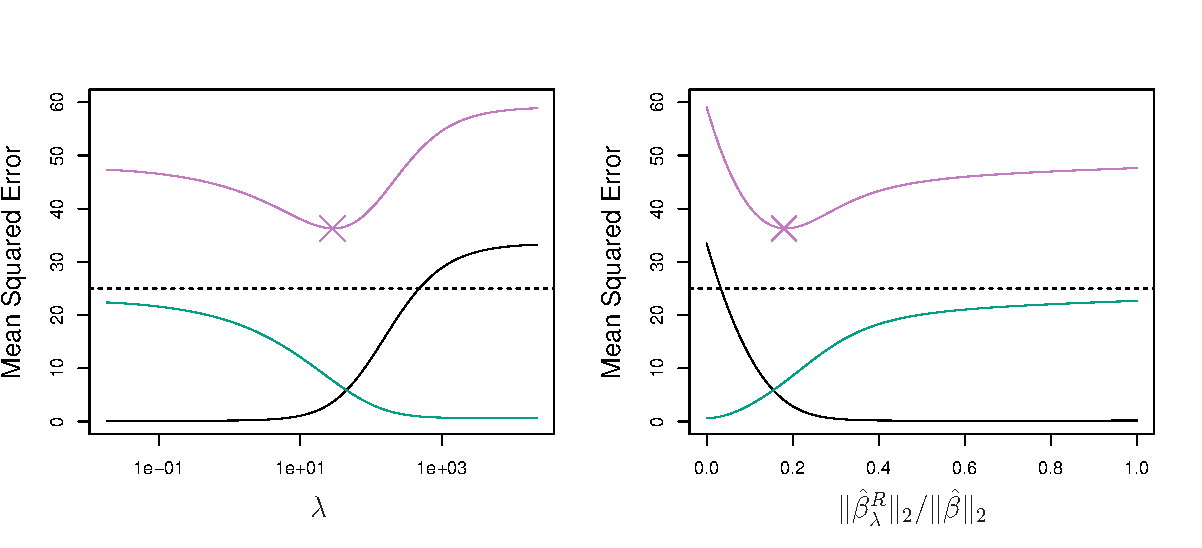
\includegraphics[width=4in]{6_5.pdf}
%\end{center}
%\vspace{-0.5cm}
%$bias^2$ (black), $variance$ ({\color{green}green}), test MSE ({\color{magenta}purple})
%
%\sko
%
%\ba \dg{Ridge is computationally very attractive as the ``computing cost'' is almost the same of least squares (contrast that with subset selection!)} \\ \sko
%\ba \dg{It's a good practice to always center and scale the $X$'s}
%
%\end{frame}
%
%
%%%%%%%%%%%%%%%%%%%%%%%%%%%%%%%%%%%%%%%
%\begin{frame}
%\frametitle{LASSO}
%The LASSO is a shrinkage method that performs automatic selection. It is similar to ridge but it will provide solutions that are {\color{red}sparse}, ie, some $\beta$'s exactly equal to 0! This facilitates interpretation of the results...
%
%\skoo
%\begin{tabular}{cc}
%Ridge & LASSO\\
%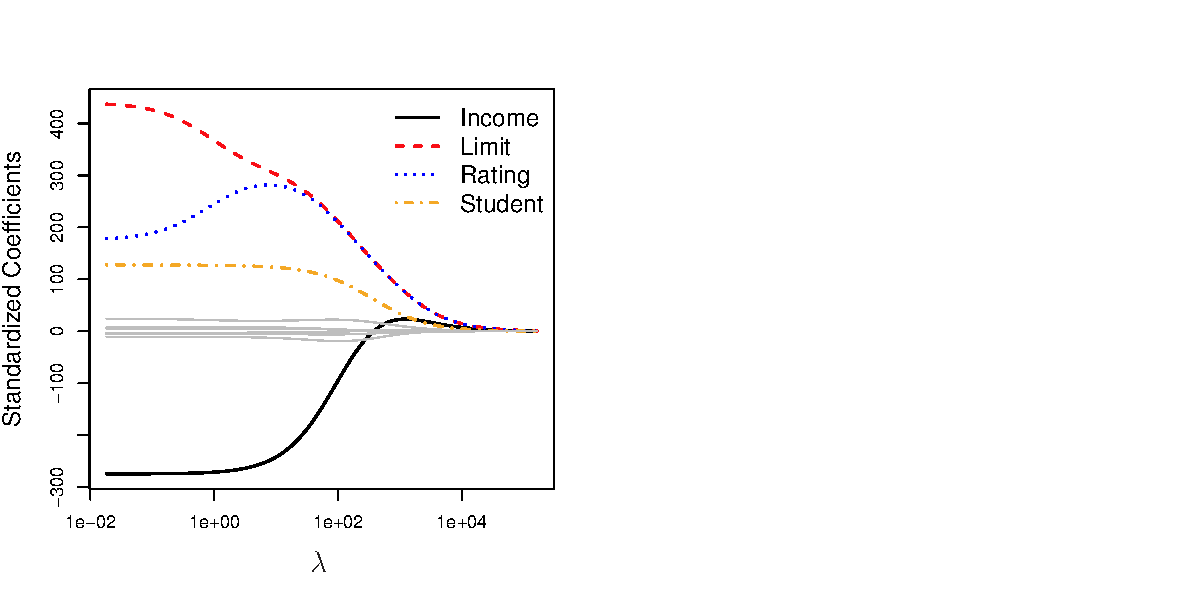
\includegraphics[width=2in]{6_4}&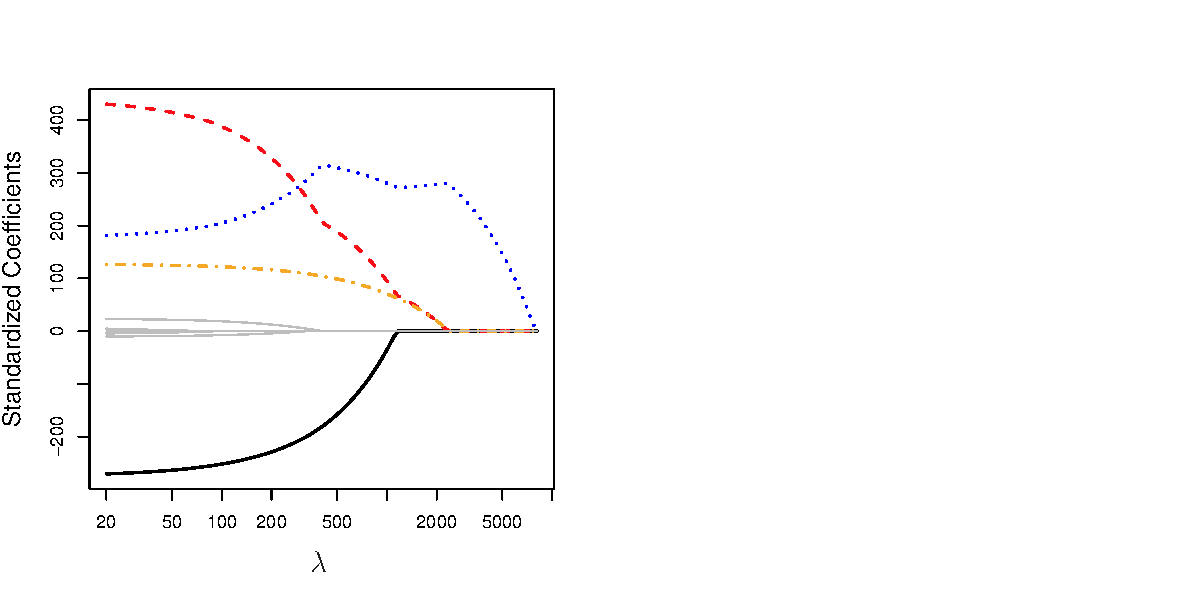
\includegraphics[width=2in]{6_6}\\
%\end{tabular}
%
%\end{frame}
%
%
%
%
%
%%%%%%%%%%%%%%%%%%%%%%%%%%%%%%%%%%%%%%%
%\begin{frame}
%\frametitle{LASSO}
%
%
%The LASSO solves the following problem:
%$$
%\mbox{arg min}_{\beta} \left\{
%{\color{lightblue}\sum_{i=1}^n \left( Y_i - \beta_0 -  \sum_{j=1}^p \beta_j X_{ij} \right)^2 }+ {\color{red}\lambda\sum_{j=1}^p |\beta_j|}  \right\}
%$$
%\bi
%\item Once again, $\lambda$ controls how flexible the model gets to be
%\item Still a very efficient computational strategy 
%\item Whenever possible, we will choose $\lambda$ by comparing the out-of-sample performance (usually via cross-validation)
%\ib 
%
%
%\sk
%
%\end{frame}
%%%%%%%%%%%%%%%%%%%%%%%%%%%%%%%%%%%%%%%
%\begin{frame}
%\frametitle{Ridge vs. LASSO}
%Why does the LASSO outputs zeros?
%\begin{center}
%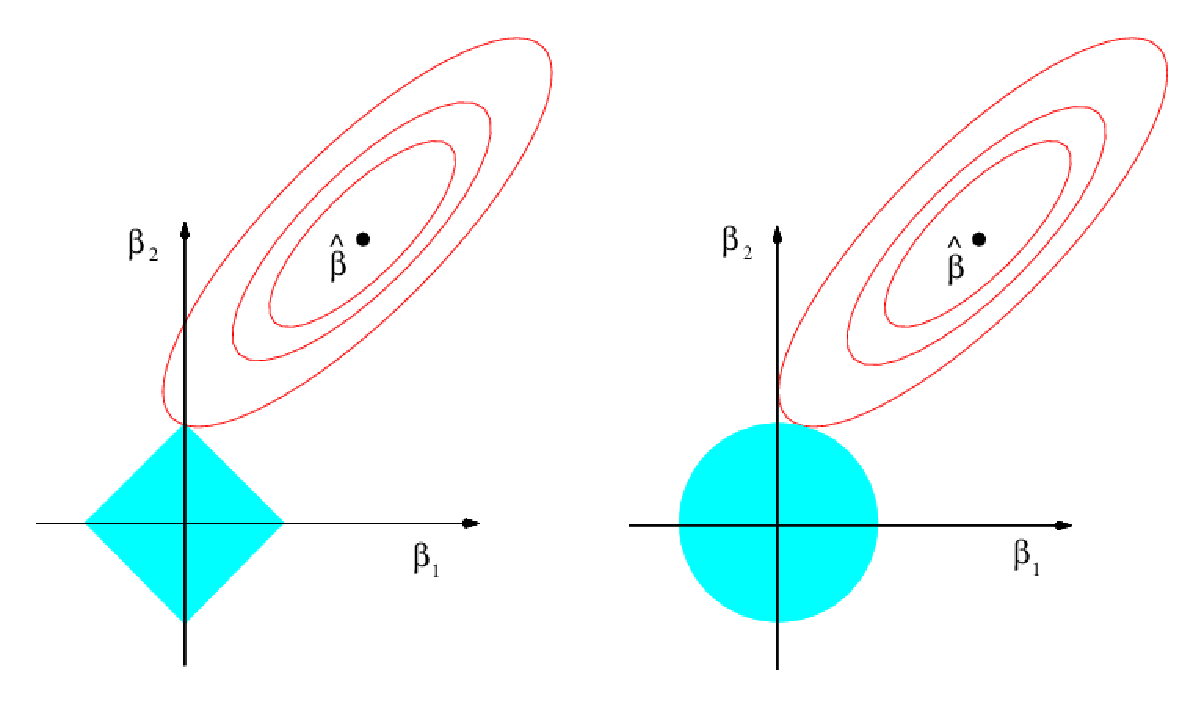
\includegraphics[width=4in]{6-7}
%\end{center}
%
%\end{frame}
%
%
%
%
%%%%%%%%%%%%%%%%%%%%%%%%%%%%%%%%%%%%%%%
%\begin{frame}
%\frametitle{Ridge vs. LASSO}
%Which one is better? \sk
%\bi
%\item \bo{\bf It depends}... 
%\item In general LASSO will perform better than Ridge when a relative small number of predictors have a strong effect in Y while Ridge will do better when Y is a function of many of the $X$'s and the coefficients are of moderate size
%\item LASSO can be easier to interpret (the zeros help!)
%\item But, if prediction is what we care about the only way to decide which method is better is comparing their out-of-sample performance
%\ib
%
%\end{frame}
%
%
%
%
%%%%%%%%%%%%%%%%%%%%%%%%%%%%%%%%%%%%%%%
%\begin{frame}
%\frametitle{Choosing $\lambda$}
%The idea is to solve the ridge or LASSO objective function over a grid of possible values for $\lambda$...
%
%
%\hspace*{-8mm}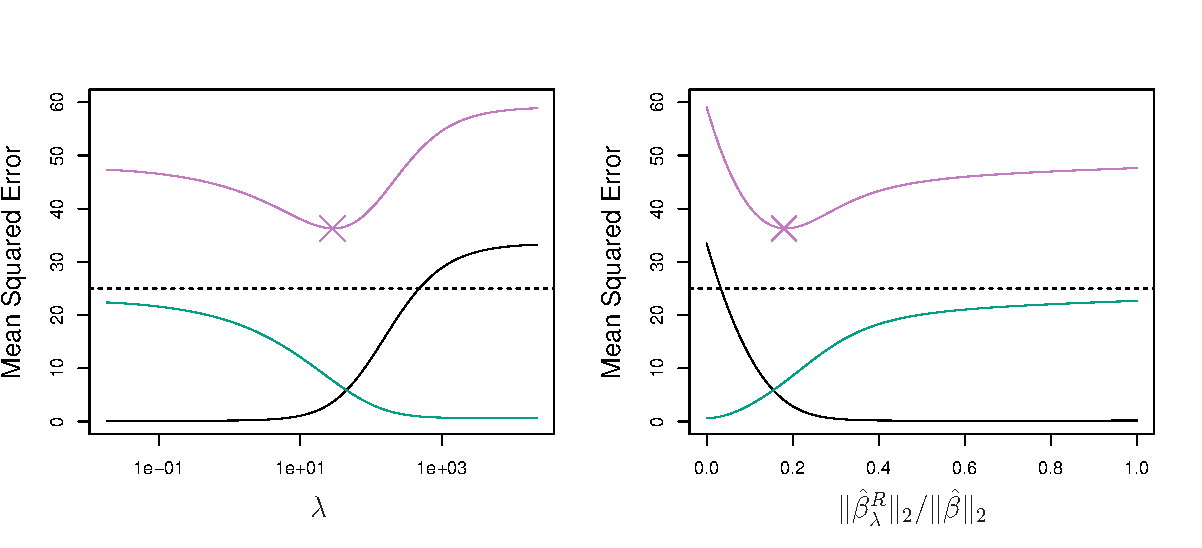
\includegraphics[width=5in]{6_5.pdf}
%
%
%\end{frame}
%
%
%\begin{frame}
%	\frametitle{How to do this in {\tt R}}
%	
%	Check out the package {\tt glmnet}.  You can easily do \bo{Ridge}, \bo{LASSO}, and much more!
%	
%\end{frame}
%
%
%\begin{frame}
%
%\sk\sk
%\dg{\Large \bf Nonlinear models (Trees) and the B-V tradeoff}
%\end{frame}
%
%\begin{frame}
%	\frametitle{Trees}
%\vspace{0mm}
%\hspace*{-2mm}
%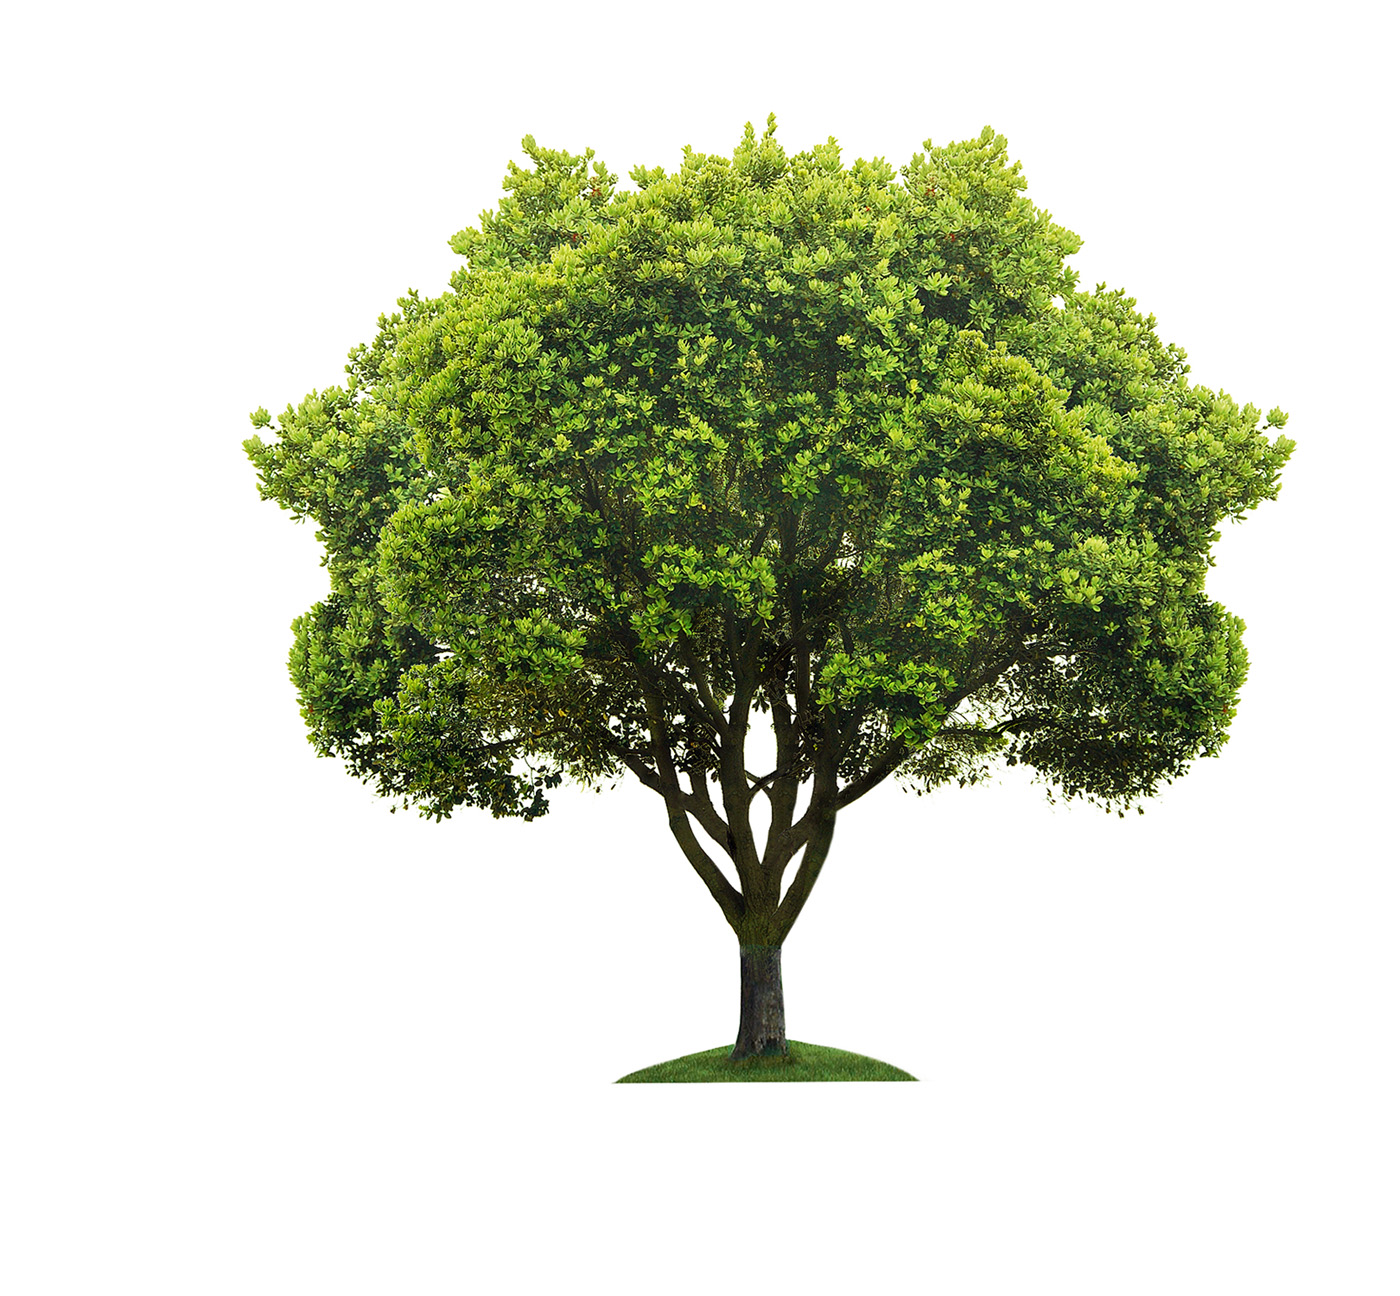
\includegraphics[scale=.88]{treepic}
%
%\end{frame}
%
%\begin{frame}[plain]
%\frametitle{Trees}
%\vspace{-10mm}
%\hspace*{8mm}
%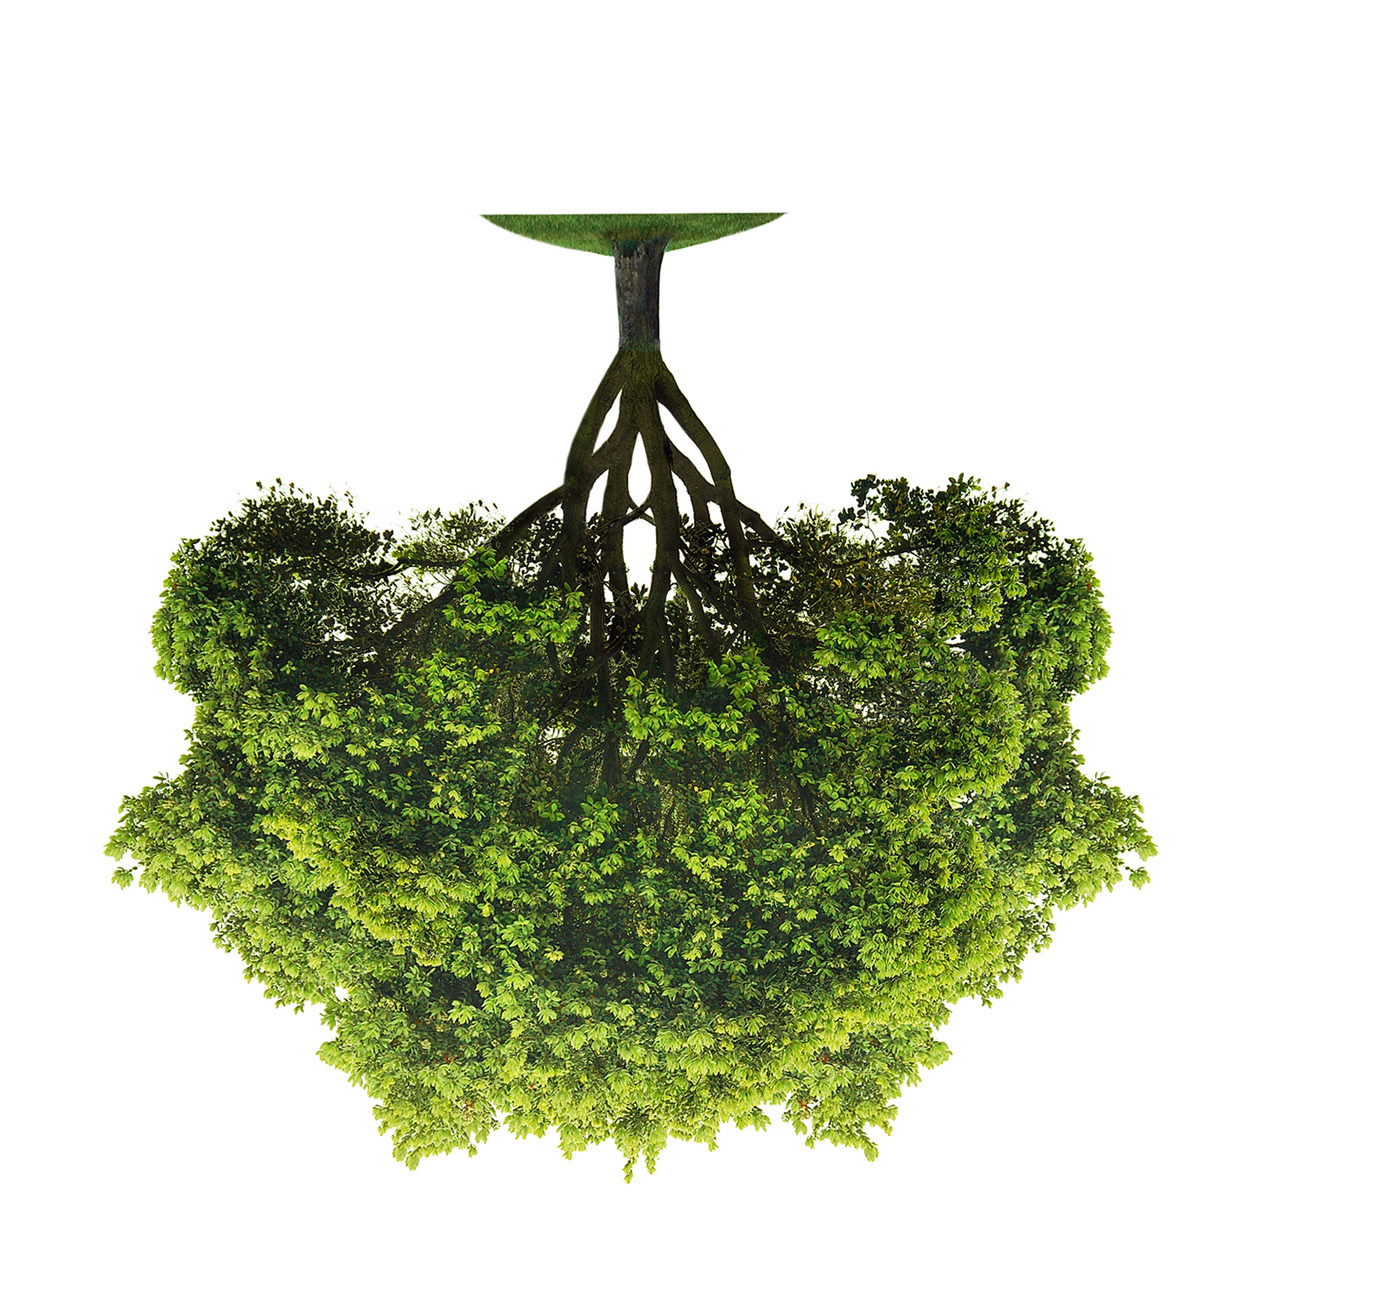
\includegraphics[scale=.88]{treepicflip}
%\end{frame}
%
%
%{
%\vspace{-5mm}
%\usebackgroundtemplate{\tikz{\node[opacity=0.01]{\hspace{12mm}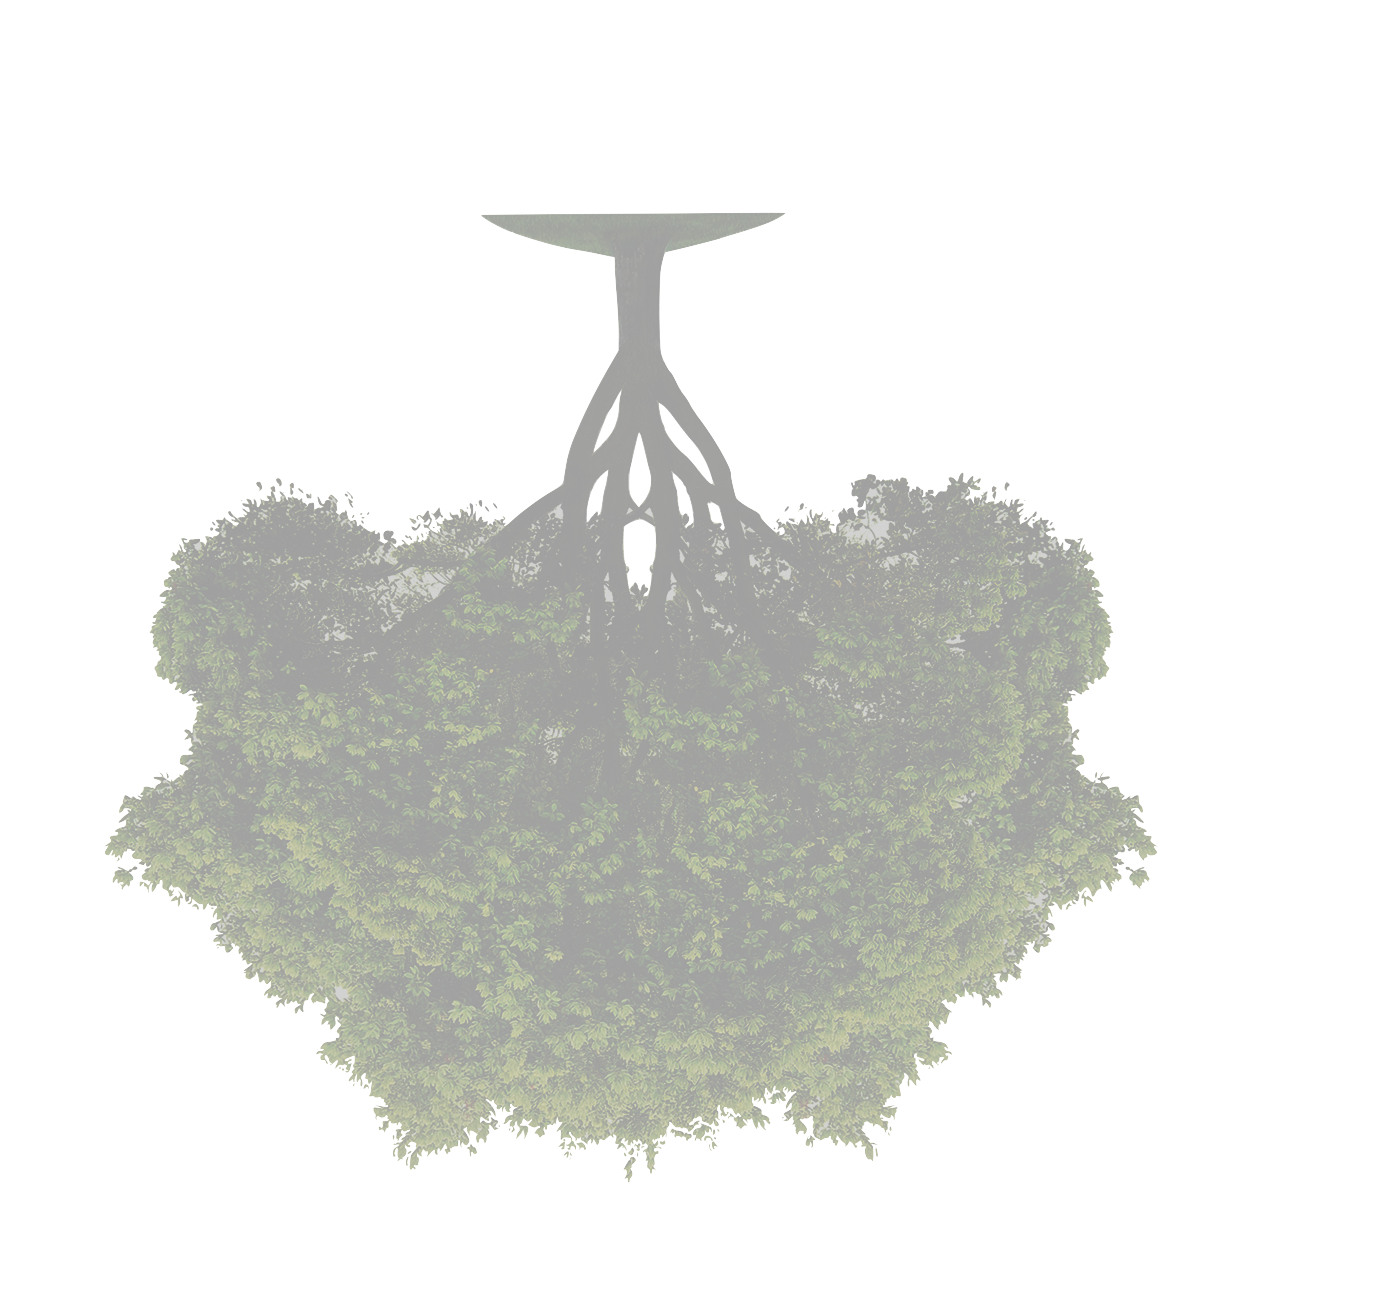
\includegraphics[scale=.93]{treepicflip2}}}}
%\begin{frame}[plain]
%\vspace{-12mm}
%\center{\it stump}
%\frametitle{Trees}
%\center{\vspace{-7mm}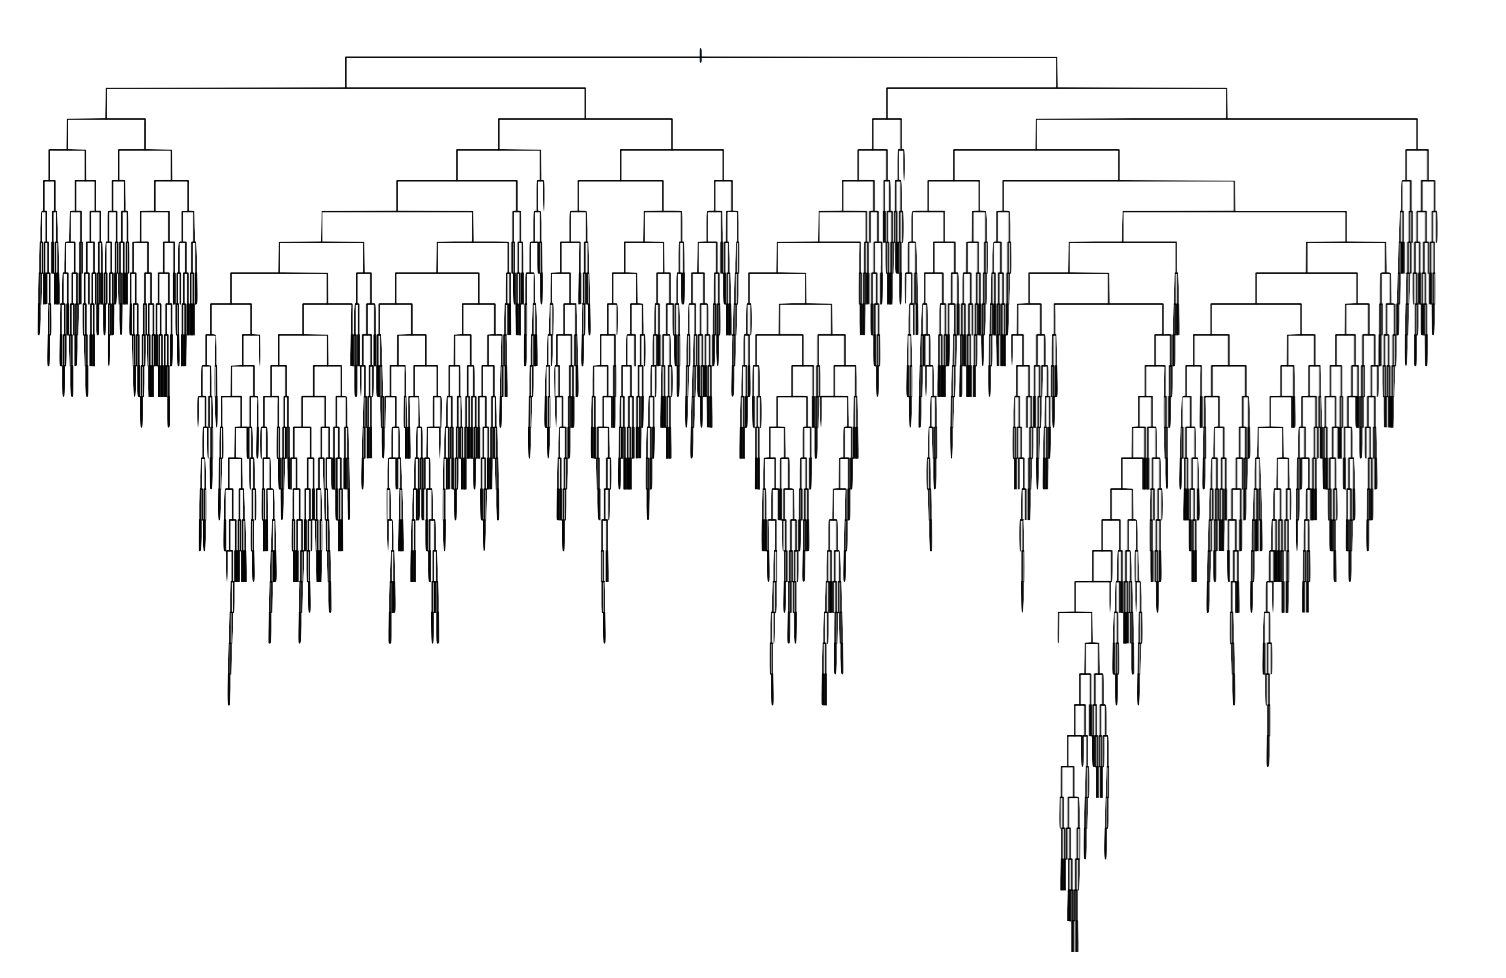
\includegraphics[scale=.435]{Bigtree}}
%\vspace{-20mm}
%\center{\it leaves}
%\end{frame}
%}
%
%
%
%\begin{frame}
%	\frametitle{Trees}
%	
%	Tree-based methods are a major player in data-mining.\skoo
%
%{\bl Good}:
%\bi
%\p flexible fitters, capture nonlinearity and interactions.
%\p do not have to think about scale of variables.
%\p handles categorical and numeric $y$ and $x$ very nicely.
%\p fast.
%\p interpretable (when small).
%\ib\skoo
%
%{\bl Bad}:
%
%Not the best in out-of-sample predictive performance\\
%\hspace*{.3in} ({\it but not bad!!}).
%
%	
%\end{frame}
%
%	
%	\begin{frame}
%
%{\Large \bl \bf However},\skoo
%
%If we {\rd \bf bag} or {\rd \bf boost}  trees, we can get the best off-the-shelf
%prediction available.\skooo
%
%Bagging and Boosting are {\bl \bf ensemble methods} that combine the fit from
%many (hundreds, thousands) of tree models to get an overall predictor.
%
%
%	
%\end{frame}
%
%
%\begin{frame}
%	\frametitle{The overall goal ...}
%	
%{\Huge \[  Y_i = f(X_i) + \epsilon_i \]} \\ \sk
%
%\hspace*{40mm}with {\Large $f = \adjincludegraphics[valign=c,scale=0.15]{treepicflip} $}
%
%
%\end{frame}
%
%\begin{frame}
%\frametitle{Back to the Boston housing data}
%	Let's look at a simple 1-dimensional example so that we can see what is going on.\sk\sk
%
%We'll use the Boston housing data and relate x=lstat to y=medval.
%\end{frame}
%
%
%\begin{frame}
%
%At left is the \bo{\bf tree} fit to the data.\sko
%
%At each \lb{\bf interior  node} there is a decision rule of the form $\{x<c\}$.\\
%If $x<c$ you go left, otherwise you go right.\sko
%
%Each observation is sent down the tree until it hits a bottom node or \lb{\bf leaf} of
%the tree.\sko
%
%\vspace{-.63in}
%
%\begin{center}
%\hspace*{-.5in} 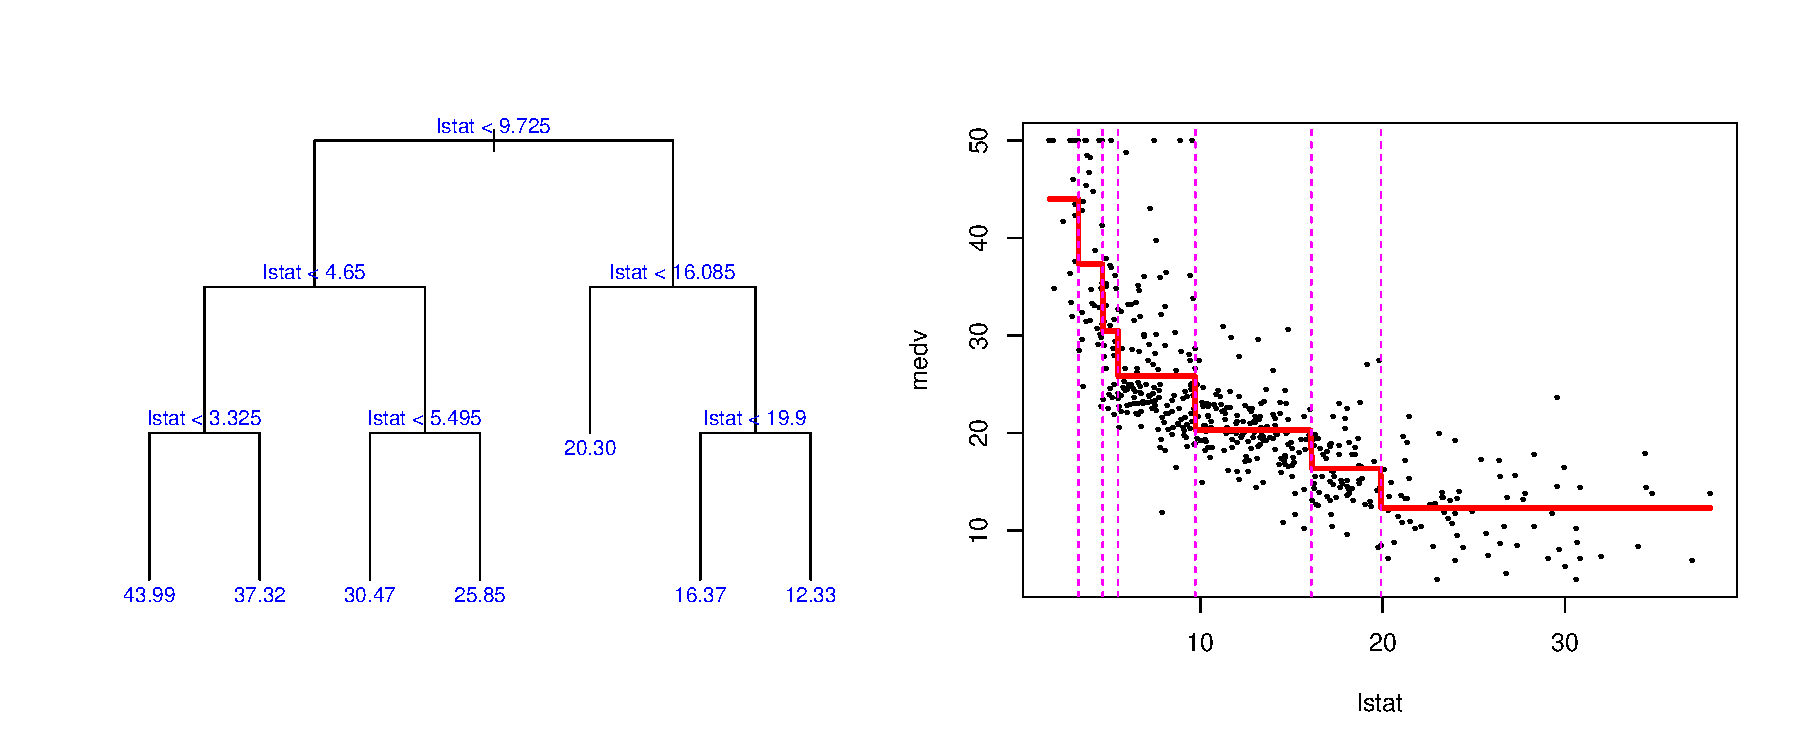
\includegraphics[scale=.4]{boston-lstat-simple-tree.pdf}
%\end{center}
%
%\vspace{-.35in}
%
%The set of bottom nodes gives us a partition of the predictor ($x$) space into disjoint regions.
%At right, the vertical lines display the partition.  With just one $x$, this is just
%a set of intervals.  
%
%\end{frame}
%%--------------------------------------------------
%\begin{frame}
%\sko
%Within each region (interval) we compute the average of the 
%$y$ values for the subset of training data in the region.
%This gives us the step function which is our $\hat{f}$. 
%The $\bar{y}$ values are also printed at left at the bottom nodes.
%
%\vspace{-.5in}
%
%\begin{center}
%\hspace*{-.5in} 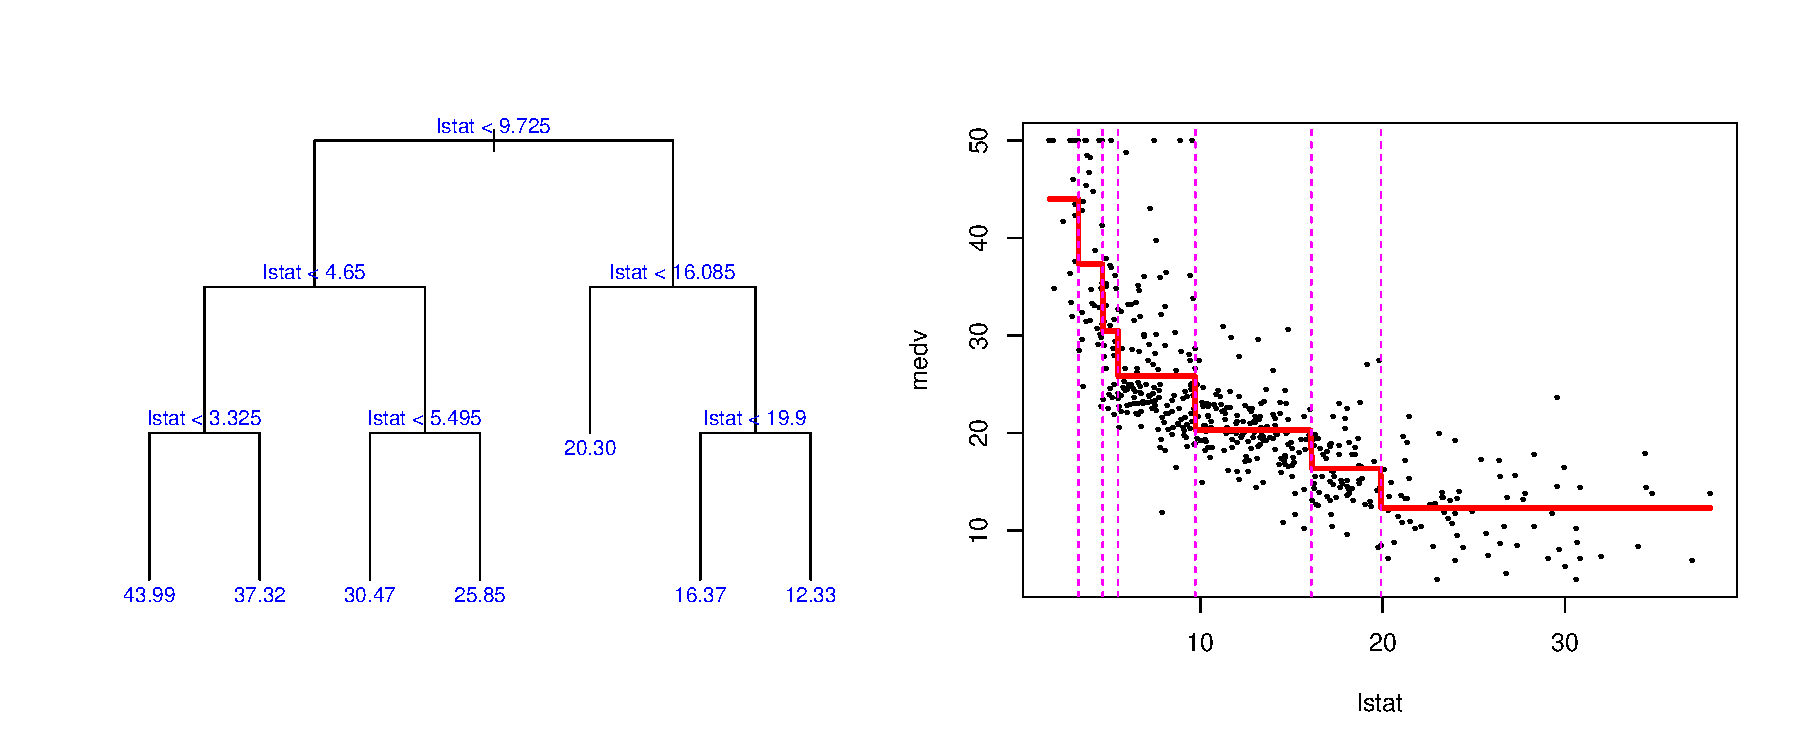
\includegraphics[scale=.4]{boston-lstat-simple-tree.pdf}
%\end{center}
%
%\vspace{-.3in}
%
%To predict, we just use our step function estimate of $f(x)$.\sko
%
%Equivalently, we drop $x$ down the tree until it lands in a leaf
%and then predict the average of the $y$ values for the training observations
%in the same leaf.\sko
%
%%{\small \color{lightgray} (See {\tt boston-lstat-simple-tree.R})}
%\end{frame}
%
%\begin{frame}
%\frametitle{Two explanatory variables}
%Here is a tree with $x=(x_1,x_2)=$ (lstat,dis) and y=medv.\sko
%
%\vspace{-.55in}
%
%\begin{center}
%\hspace*{-.3in} 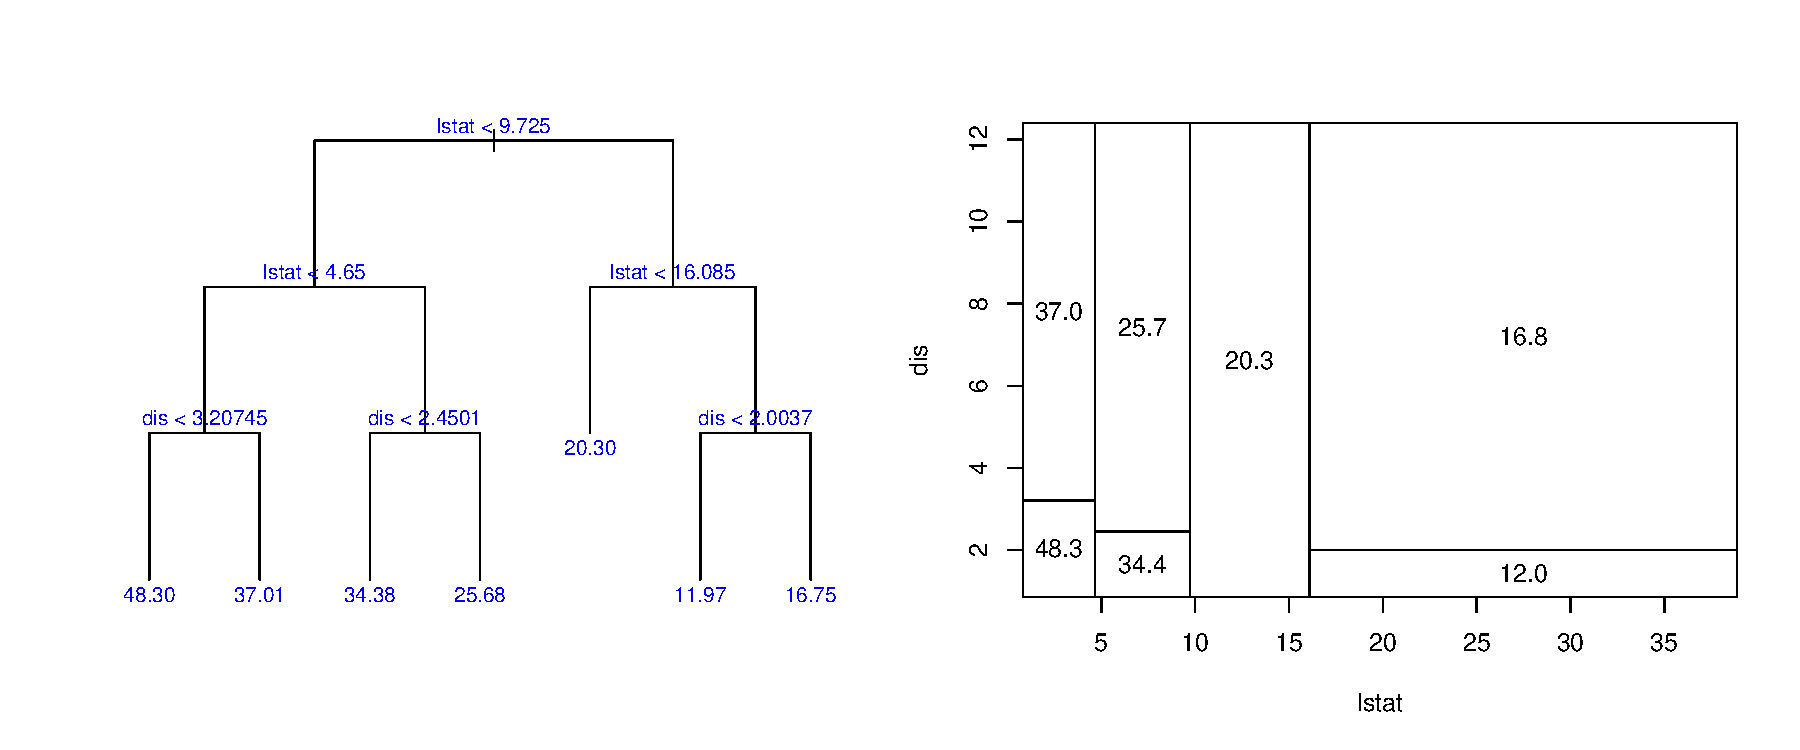
\includegraphics[scale=.4]{boston-lstat-dis-simple-tree.pdf}
%\end{center}
%
%\vspace{-.2in}
%
%At right is the {\it partition} of the $x$ space corresponding to the set of
%bottom nodes (leaves).\sko
%
%The average $y$ for training observations assigned to a region is printed in
%each region and at the bottom nodes.
%
%
%\end{frame}
%
%%--------------------------------------------------
%\begin{frame}
%\frametitle{The regression function in 2-D!}
%
%\begin{minipage}{1.5in}
%{\footnotesize
%This is the regression function given by the tree.\sko
%
%It is a step function which can seem stupid,
%but it delivers nonlinearity {\it and} interactions in
%a simple way and works with a lot of variables.\sko
%
%Notice the interaction.\\
%The effect of {\tt dis} depends on {\tt lstat}!!
%}
%\end{minipage}
%\hspace*{-.2in}
%\begin{minipage}{2.0in}
%\begin{center}
%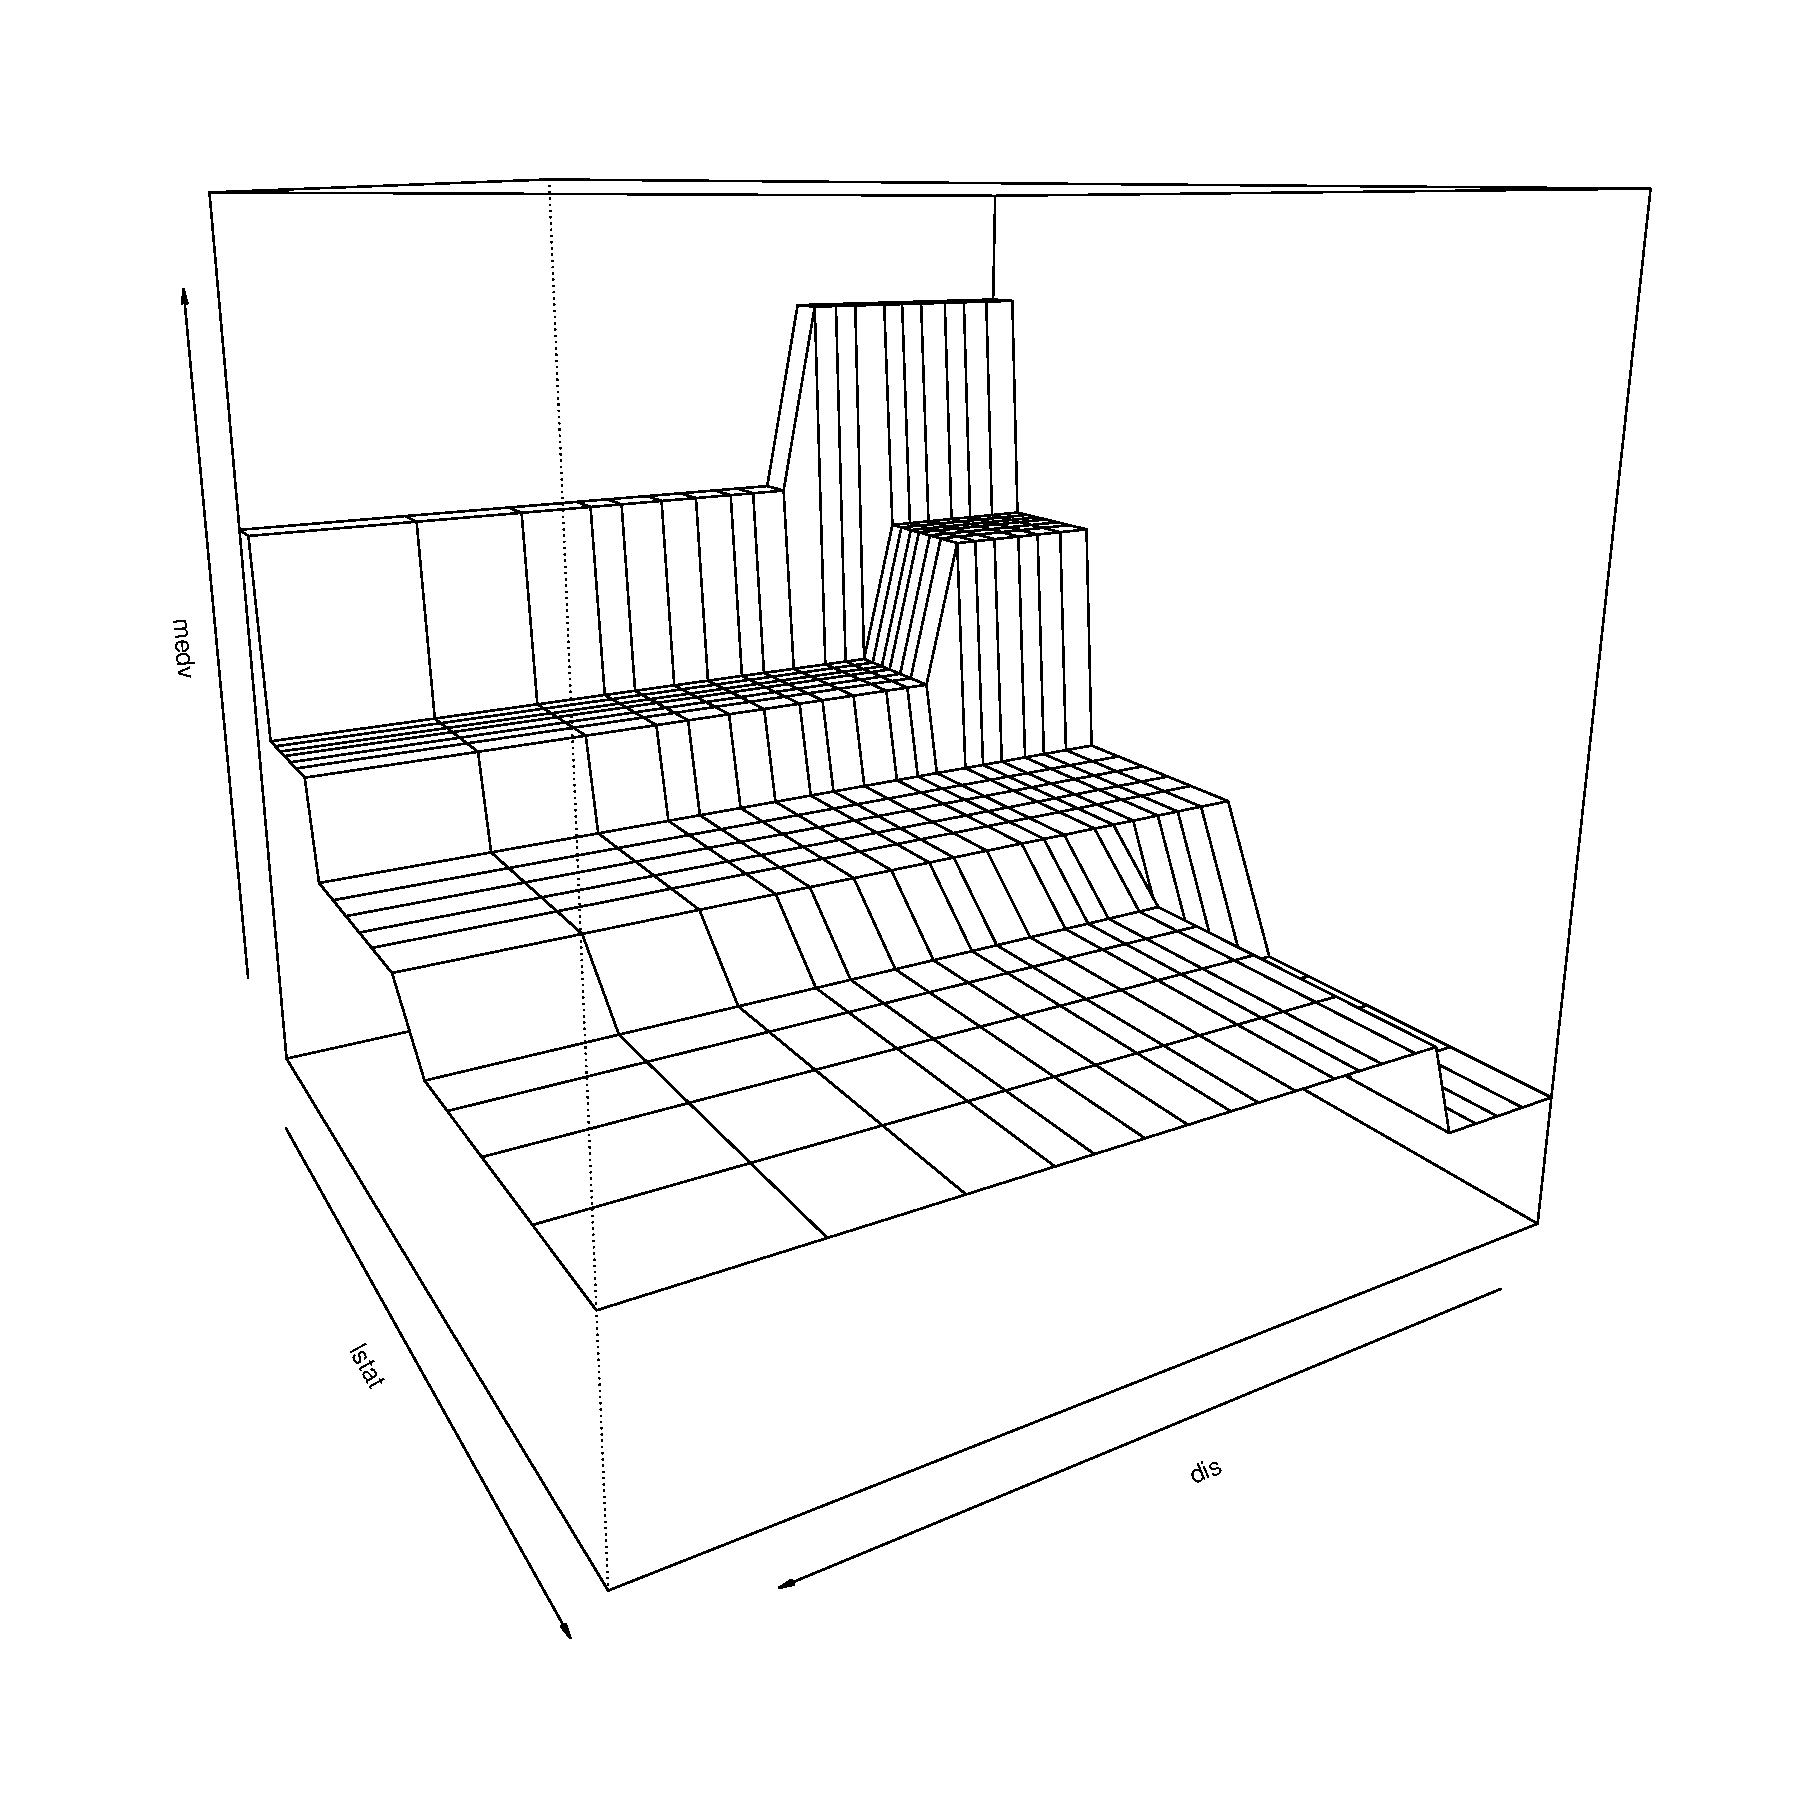
\includegraphics[scale=.28]{boston-lstat-dis-persp.pdf}
%\end{center}
%\end{minipage}
%
%\vspace{-.2in}
%
%%{\small \color{lightgray} (See {\tt boston-lstat-dis-persp.R})}
%
%\end{frame}
%
%
%\begin{frame}
%\frametitle{Tree models and the bias variance tradeoff}
%
%How do we fit trees to data??\skooo
%
%The key idea is that a {\color{red}complex} tree is  a {\color{red}big} tree.\skoo
%
%We usually measure the complexity of the tree by the number of bottom nodes.
%
%\end{frame}
%%--------------------------------------------------
%\begin{frame}
%\frametitle{Minimizing a penalized loss}
%To fit a tree, we try to minimize:
%
%$$
%C(T,y) = L(T,y) + \alpha \, |T|
%$$
%
%where,\skoo
%
%\bi
%\p $L(T,y)$ is our loss in fitting data $y$ with tree $T$.
%\p $|T|$ is the number of bottom nodes in tree $T$.
%\ib\skoo
%
%For numeric $y$ our loss is usually {\color{red}sum of squared errors}, for categorical
%$y$ we can use the {\color{red}deviance} or the {\color{red}miss-classification rate}.\skoo
%
%Note: $\alpha$ is analogous to the lasso $\lambda$ !!!
%\end{frame}
%%--------------------------------------------------
%\begin{frame}
%
%{\bl \Large How do we do the minimization?}
%
%\vspace{.3in}
%
%Now we have a problem.\skooo
%
%While trees are simple in some sense, once we view them as variables
%in an optimization they are large and complex.\skooo
%
%A key to tree modeling is the success of the following heuristic algorithm
%for fitting trees to training data.
%\end{frame}
%%--------------------------------------------------
%\begin{frame}
%
%{\bl (I. Grow Big)}\sko
%
%Use a greedy, recursive forward search to build a big tree.\sko
%
%{\rd (i)}\sko
%
%Start with the tree that is a single node.\skoo
%
%{\rd (ii)}\sko
%
%At each bottom node, search over all possible decision rules to find the one
%that gives the biggest decrease in loss (increase in fit).  \skoo
%
%{\rd (iii)}\sko
%
%Grow a big tree, stopping (for example) when each bottom node has 5 observations
%in it.
%\end{frame}
%%--------------------------------------------------
%\begin{frame}
%
%{\bl (II. Prune Back)}\sko
%
%
%{\rd (i)}\sko
%
%Recursively, prune back the big tree from step (I).\skoo
%
%{\rd (ii)}\sko
%
%Give a current pruned tree, examine every pair of bottom nodes (having the same parent node)
%and consider eliminating the pair.\sko 
%
%Prune the pair the gives the biggest decrease in our criterion $C$.\sko
%
%This is give us a sequence of subtrees of our initial big tree.\skoo
%
%{\rd (iii)}\sko
%
%For a given $\alpha$, choose the subtree of the big tree that has the smallest $C$.
%\end{frame}
%
%
%\begin{frame}
%
%{\bl \bf So,}\skoo
%
%Give training data and $\alpha$ we get a tree.\skoo
%
%{\rd \bf How do we choose $\alpha$?}\skoo
%
%As usual, we can leave out a validation data set and choose the $\alpha$ the performs
%best on the validation data, or use k-fold cross validation.
%\end{frame}
%%--------------------------------------------------
%\begin{frame}
%
%\begin{minipage}{1.2in}
%{\scriptsize
%On the right are three different tree fits
%we get from three different $\alpha$ values
%(using all the data).
%
%\vspace{.2in}
%
%The smaller $\alpha$ is,
%the lower the penalty for complexity is,
%the bigger tree you get.\skoo
%
%The top tree is a sub-tree of the middle tree,
%and the middle tree is a sub-tree of the bottom tree.\skoo
%
%
%
%The middle $\alpha$ is the one suggested by CV.
%
%}
%\end{minipage}
%\hspace*{.3in}
%\begin{minipage}{2.0in}
%\begin{center}
%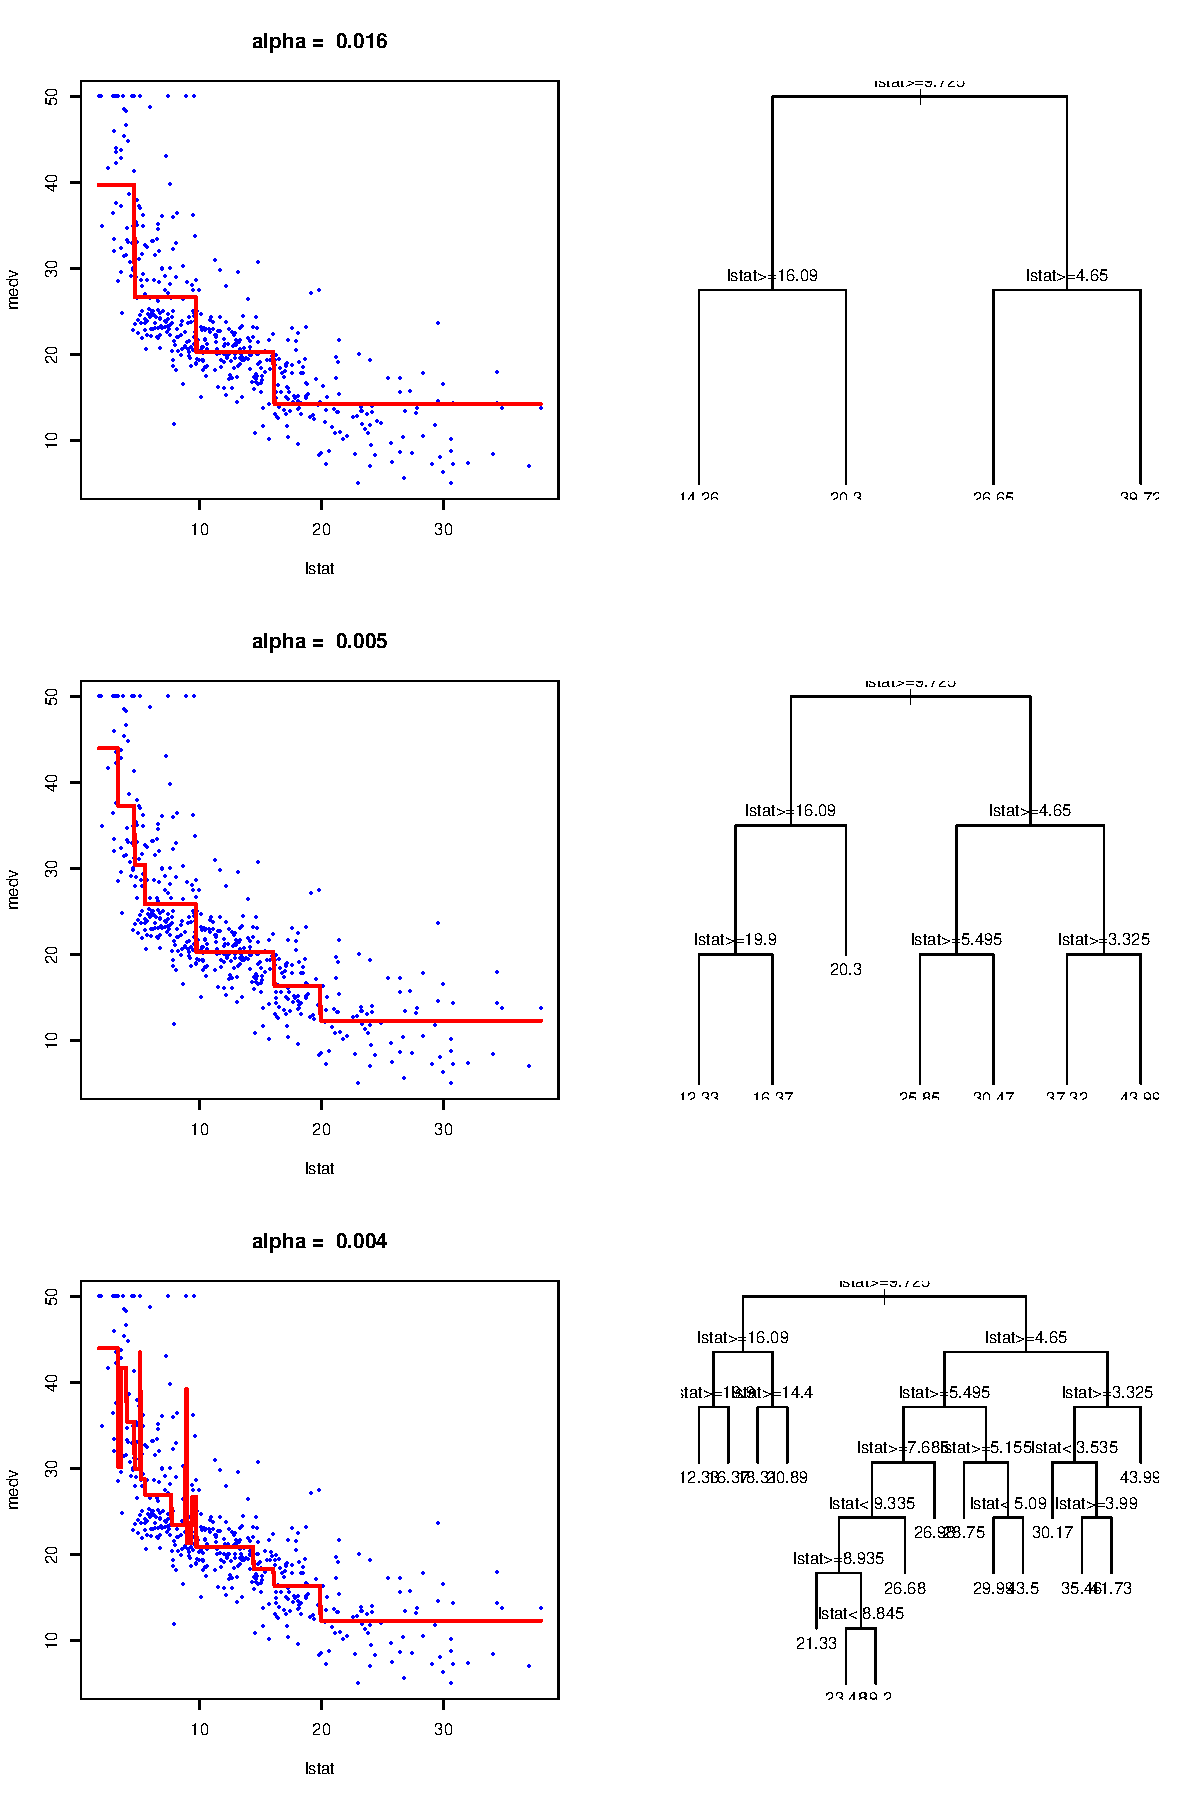
\includegraphics[scale=.32]{boston-lstat-rpart-plotfits.pdf}
%\end{center}
%\end{minipage}
%
%\end{frame} 
%
%
%\begin{frame}
%	\frametitle{What are the models data scientists use today?}
%	
%	\bb \dg{Random forests} \\ \sk
%	\bb \dg{Boosting and Bagging trees} \\ \sk
%	\bb \bo{\bf Bayesian additive regression trees (BART)} \\ \sko
%	\hspace*{3mm}\ba tree growth is probabilistic \\ \sko
%	\hspace*{3mm}\ba regularization is ``baked into'' the priors
%	
%\end{frame}


\begin{frame}
	\frametitle{What have we learned?}
	
	More \bo{wiggles} are not always better! \\ \sko \sko \sk
	
	A function fit to data should be ``adaptive enough.'' \\ \sko \sko \sk
	
	If too adaptive \dg{aka} \textbf{overfit} to the \lb{observed} data, it will not predict well when confronted with \lb{new} data.
	
	
	
\end{frame}


\end{document} 











